\documentclass[11pt,a4paper,onecolumn,twoside,ngerman]{book}

% Konfiguration laden
% header.tex

\usepackage[a4paper,left=3.5cm,right=2.5cm,bottom=3cm,top=3cm]{geometry}
\usepackage[ngerman,english]{babel}
\usepackage{graphicx}
\usepackage{color}
\usepackage{import}
\usepackage{amsmath,amssymb}

\usepackage[numbers]{natbib}% von Author hinzugefügt
%\usepackage{amsmath,amssymb,subfigure}
 
\usepackage{verbatim} % von Autor ergänzt

\usepackage{needspace}% für itemize seiten neu

%%%%%%%%%%%%%%%%%%%%%%%%%%%%%%%%%%%%%%%%%%%%%%%%%%%%%%%%
\usepackage{wasysym} % für das checked symbol Häkchen
% für Farben im allgemeinen
\usepackage[table]{xcolor}
\usepackage{tabularx}
\usepackage{colortbl}	

\usepackage{array,longtable}
\usepackage[alwaysadjust]{paralist}
\setdefaultitem{\textbullet}{\textbullet}{\textbullet}{\textbullet}

%%%%%%%%%%%%%%%%%%%%%%%%%%%%%%%%%%%%%%%%%%%%%%%%%%%%%%

% Theorem-Umgebungen
\usepackage[amsmath,thmmarks]{ntheorem}
%\usepackage{svg}
% Korrekte Darstellung der Umlaute
\usepackage[utf8]{inputenc}
\usepackage[T1]{fontenc}
\usepackage{microtype}% verbesserter Randausgleich
\usepackage[autostyle=true,german=quotes]{csquotes}
% Algorithmen
\usepackage[plain,chapter]{algorithm}
\usepackage{algorithmic}
\usepackage{enumerate}
%Abkürzungsvereichnis
\usepackage[printonlyused]{acronym}

%PDF anhängen
\usepackage{pdfpages}

% Bibtex deutsch
\usepackage{bibgerm}
%Crossrodes referenzes
\usepackage{xr}
% URLs
\usepackage{url}
%notes und grafiken
\usepackage[ngerman]{todonotes}
\setlength{\marginparwidth}{2cm}
%Liste im Text
\usepackage{paralist}
% Caption Packet
\usepackage[margin=0pt,font=small,labelfont=bf]{caption}
\usepackage[labelformat=simple]{subcaption}
\renewcommand\thesubfigure{(\alph{subfigure})} 
%\usepackage[margin=0pt,font=small,labelfont=bf]{subcaption}
% Gliederung einstellen
%\setcounter{secnumdepth}{5}
%\setcounter{tocdepth}{5}

\usepackage[explicit]{titlesec}
\usepackage{lmodern}
\usepackage{lipsum}
\definecolor{mygreen}{rgb}{0,0.6,0}
\definecolor{mygray}{rgb}{0.5,0.5,0.5}
\definecolor{mymauve}{rgb}{0.58,0,0.82}
\definecolor{pl_background}{rgb}{0.95,0.95,0.95}
\definecolor{pl_comment}{rgb}{0.12, 0.38, 0.18 }
\definecolor{pl_ifelse}{rgb}{0.74,0.74,.29}
\definecolor{pl_keyword}{rgb}{0.37, 0.08, 0.25}
\definecolor{pl_string}{rgb}{0.06, 0.10, 0.98}

%\usepackage{listings}

\usepackage{listings,xcolor}
% Vordefiniertes Programmlisting
\lstdefinestyle{myCustomJavaStyle}{
%\lstset{
language = java,
basicstyle = \small\sffamily,
backgroundcolor = \color{pl_background},
stringstyle = \color{pl_string},
keywordstyle = \color{pl_keyword}\bfseries,
commentstyle = \color{pl_comment}\itshape,
frame = lrbt,
numbers = left,
showstringspaces = false,
breaklines = true,
xleftmargin = 15pt
%emph = [1]{java},
%emphstyle = [1]\color{black},
%emph = [2]{if,and,or,else},
%emphstyle = [2]\color{pl_keyword}
}

\lstdefinestyle{myCustomMatlabStyle}{
  language=java,
  numbers=left,
  stepnumber=1,
  numbersep=8pt,
  tabsize=2,
  showspaces=false,
  showstringspaces=true,
  backgroundcolor=\color{white},
  basicstyle=\footnotesize,
  commentstyle=\itshape\color{blue!90!black},
  keywordstyle=\bfseries\color{red!40!black},
  %identifierstyle=\color{black},
  %stringstyle=\color{blue}
  %keywordstyle=\color{black}
}

%\usepackage{rotating}%rotation der Tabelle Autor
%\usepackage{pdflscape} %Autor


% Abstand swischen zwei Absätzen
%\parskip=0.5em
%\setlength{\parindent}{0pt}


\newlength\chapnumb
\setlength\chapnumb{2.5cm}

\titleformat{\chapter}[block]
{\normalfont\sffamily}{}{0pt}
{\parbox[b]{\chapnumb}{%
   \fontsize{80}{70}\selectfont\thechapter}%
  \parbox[b]{\dimexpr\textwidth-\chapnumb\relax}{%
    \raggedleft%
    \hfill{\LARGE#1}\\
    \rule{\dimexpr\textwidth-\chapnumb\relax}{0.4pt}}}
\titleformat{name=\chapter,numberless}[block]
{\normalfont\sffamily}{}{0pt}
{\parbox[b]{\dimexpr\textwidth\relax}{%
    \raggedleft%
    \hfill{\LARGE#1}\\
    \rule{\dimexpr\textwidth\relax}{0.4pt}}}

% Theorem-Optionen %
\theoremseparator{.}
\theoremstyle{change}
\newtheorem{theorem}{Theorem}[section]
\newtheorem{satz}[theorem]{Satz}
\newtheorem{lemma}[theorem]{Lemma}
\newtheorem{korollar}[theorem]{Korollar}
\newtheorem{proposition}[theorem]{Proposition}
% Ohne Numerierung
\theoremstyle{nonumberplain}
\renewtheorem{theorem*}{Theorem}
\renewtheorem{satz*}{Satz}
\renewtheorem{lemma*}{Lemma}
\renewtheorem{korollar*}{Korollar}
\renewtheorem{proposition*}{Proposition}
% Definitionen mit \upshape
\theorembodyfont{\upshape}
\theoremstyle{change}
\newtheorem{definition}[theorem]{Definition}
\theoremstyle{nonumberplain}
\renewtheorem{definition*}{Definition}
% Kursive Schrift
\theoremheaderfont{\itshape}
\newtheorem{notation}{Notation}
\newtheorem{konvention}{Konvention}
\newtheorem{bezeichnung}{Bezeichnung}
\theoremsymbol{\ensuremath{\Box}}
\newtheorem{beweis}{Beweis}
\theoremsymbol{}
\theoremstyle{change}
\theoremheaderfont{\bfseries}
\newtheorem{bemerkung}[theorem]{Bemerkung}
\newtheorem{beobachtung}[theorem]{Beobachtung}
\newtheorem{beispiel}[theorem]{Beispiel}
\newtheorem{problem}{Problem}
\theoremstyle{nonumberplain}
\renewtheorem{bemerkung*}{Bemerkung}
\renewtheorem{beispiel*}{Beispiel}
\renewtheorem{problem*}{Problem}

% Algorithmen anpassen %
\renewcommand{\algorithmicrequire}{\textit{Eingabe:}}
\renewcommand{\algorithmicensure}{\textit{Ausgabe:}}
\floatname{algorithm}{Algorithmus}
\renewcommand{\listalgorithmname}{Algorithmenverzeichnis}
\renewcommand{\algorithmiccomment}[1]{\color{grau}{// #1}}

% Zeilenabstand einstellen %
\renewcommand{\baselinestretch}{1.25}

% Floating-Umgebungen anpassen %
\renewcommand{\topfraction}{0.9}
\renewcommand{\bottomfraction}{0.8}

% Markierte Referenzen werden ausgeblendet
\usepackage[pdfborder={0 0 0}]{hyperref}
% Abkuerzungen richtig formatieren %
\usepackage{xspace}

% Leere Seite ohne Seitennummer, naechste Seite rechts
\newcommand{\blankpage}{ \clearpage{\pagestyle{empty}\cleardoublepage}}
%\newcommand{\blankpage}{ \clearpage{\pagestyle{empty}\clearpage}}

% Keine einzelnen Zeilen beim Anfang eines Abschnitts (Schusterjungen)
\clubpenalty = 10000

% Keine einzelnen Zeilen am Ende eines Abschnitts (Hurenkinder)
\widowpenalty = 10000 
\displaywidowpenalty = 10000

% EOF


% Shortcuts laden

\newcommand{\RM}[1]{\MakeUppercase{\romannumeral #1{.}}}
\newcommand{\vgl}{vgl.\@\xspace} 
\newcommand{\zB}{z.\nolinebreak[4]\hspace{0.125em}\nolinebreak[4]B.\@\xspace}
\newcommand{\bzw}{bzw.\@\xspace}
\newcommand{\dahe}{d.\nolinebreak[4]\hspace{0.125em}h.\nolinebreak[4]\@\xspace}
\newcommand{\etc}{etc.\@\xspace}
\newcommand{\evtl}{evtl.\@\xspace}
\newcommand{\ggf}{ggf.\@\xspace}
\newcommand{\bzgl}{bzgl.\@\xspace}
\newcommand{\so}{s.\nolinebreak[4]\hspace{0.125em}\nolinebreak[4]o.\@\xspace}
\newcommand{\iA}{i.\nolinebreak[4]\hspace{0.125em}\nolinebreak[4]A.\@\xspace}
\newcommand{\sa}{s.\nolinebreak[4]\hspace{0.125em}\nolinebreak[4]a.\@\xspace}
\newcommand{\su}{s.\nolinebreak[4]\hspace{0.125em}\nolinebreak[4]u.\@\xspace}
\newcommand{\ua}{u.\nolinebreak[4]\hspace{0.125em}\nolinebreak[4]a.\@\xspace}
\newcommand{\og}{o.\nolinebreak[4]\hspace{0.125em}\nolinebreak[4]g.\@\xspace}
\newcommand{\oBdA}{o.\nolinebreak[4]\hspace{0.125em}\nolinebreak[4]B.\nolinebreak[4]\hspace{0.125em}d.\nolinebreak[4]\hspace{0.125em}A.\@\xspace}
\newcommand{\OBdA}{O.\nolinebreak[4]\hspace{0.125em}\nolinebreak[4]B.\nolinebreak[4]\hspace{0.125em}d.\nolinebreak[4]\hspace{0.125em}A.\@\xspace}

\newcommand{\rl}{reinforcement learning\@\xspace}
\newcommand{\Rl}{Reinforcement learning\@\xspace}
\newcommand{\et}
{Eyetracking-System\@\xspace}
\newcommand{\etp}
{Eyetracking-Systeme\@\xspace}
\newcommand{\tp}
{Telepräsenzrobotersystem\@\xspace}
\newcommand{\tpp}
{Telepräsenzrobotersysteme\@\xspace}
\newcommand{\iV}
{iView X\textsuperscript{TM}\@\xspace}
\newcommand{\spb}{stimuluspräsentierend Bildschirm\@\xspace}
\newcommand\mathplus{+}

% Das Hauptdokument
\begin{document}

  % Sprache
  \selectlanguage{ngerman}
  
  % Titelseite
\begin{titlepage}
\sffamily

% ---------------------------------------------------------------------
% FernUni-Logo
% ---------------------------------------------------------------------
\noindent%
\begin{minipage}{12cm}

\includegraphics[width=8cm]{bilder/titelseite/fu-signet-rgb}
\end{minipage}

% ---------------------------------------------------------------------
% Titel-Block
% ---------------------------------------------------------------------
\vspace*{4cm}%
\noindent\hspace*{1cm}%
\begin{minipage}{13cm}
\large
\begin{center}
{\Large Abschlussarbeit} \\
{\large im Studiengang Bachelor of Science in Informatik} \\
\vspace*{1cm}
\textbf{Entwicklung einer Steuerung für mobile Roboter mithilfe eines Eyetrackers} \\ %Prototyp eines Basiskommunikationssystems f"ur sprach- und bewegungseingeschr"ankte Personen \\
\vspace*{1cm}
Karl Gottfried\\
April 2017
\end{center}
\end{minipage}
\normalsize

% ---------------------------------------------------------------------
% Gutachten
% ---------------------------------------------------------------------
\vspace*{6.6cm}%
\noindent%
\begin{minipage}[b]{12cm}
\raggedright
%\textbf{Gutachten} \\
%Erstgutachterin: Prof. Dr. Gabriele Peters\\
%Zweitgutachter Prof. Dr. Christoph Beierle \\
Gutachterin: Prof. Dr. Gabriele Peters\\
Betreuung: Prof. Dr. Gabriele Peters, Prof. Dr. Christoph Beierle\\
\end{minipage}

% ---------------------------------------------------------------------
% Lehrgebiet
% ---------------------------------------------------------------------
\vspace*{2.5cm}%
\noindent%
\begin{minipage}[b]{12cm}
\raggedright
FernUniversit"at in Hagen \\
Fakult"at f"ur Mathematik und Informatik \\
Lehrgebiet Mensch-Computer-Interaktion \\
\end{minipage}
\end{titlepage}

  \blankpage

  % römischen Seitenzahlen
  \pagenumbering{roman}

  % Inhaltsverzeichnis
  \tableofcontents
  \cleardoublepage

  % Bitte die folgende Zeile stehen lassen
\newgeometry{left=5cm,right=2.5cm,bottom=4cm,top=4cm}
\chapter*{Zusammenfassung}
\vspace*{-2.5em}
%Funktionseinschränkung beider Arme und beider Beine betrafen in Deutschland Ende 2015 laut des Statistischen Bundesamt insgesamt 89088 Personen \cite{STAT2015}.
Im Rahmen der vorliegenden Abschlussarbeit konnte eine Steuerung für einen Softwareprototyp realisiert werden, die es ermöglicht, mithilfe definierter Augengesten (Blickgeste, Fixation, Lidschluss, vertikale Augenbewegung) einen vom Benutzer entfernten beweglichen Roboter zu steuern. Hierbei ermöglicht eine am Roboter angebrachte Kamera eine \enquote{Live-Ansicht} der Umgebung aus \enquote{Sicht} des Roboters, die dem Benutzer auf einem Bildschirm präsentiert wird. Der mobile Roboter fungiert somit als \acf{tps} und erweitert den Blickbereich des Benutzers auf den des \acs{tps}. Aufseiten des Benutzers entsteht das Gefühl, sich in dieser entfernten Umgebung \textit{präsent} zu fühlen, obwohl er dies nicht ist. 

Die vom System bereitgestellte Augengestenerkennung erfolgt mittels eines videobasierten stationären Eyetracking-Systems, das die aktuelle Blickposition des Benutzers, bezeichnet als \acf{por}, berechnet. Mithilfe des berechneten \acs{por} konnte durch fünf freiwillige Nutzer in einem der Modi des Prototyps die aktive Steuerung des mobilen Roboters durch einen Parcours erfolgen. Anschließend wurden die Nutzer gebeten, einen Fragebogen auszufüllen, anhand dessen zwei unterschiedliche Steuermodelle und ihre Vor- \bzw Nachteile in Bezug auf die Handhabung, die Machbarkeit und die Präzision einer derartigen Mensch-Roboter-Interaktion. Ferner konnte mittels des Fragebogens abgeschätzt werden, wie ermüdend die beiden Arten der Steuerung sind. Außerdem wurde eine Art \enquote{Panikschalter}, der einen sofortigen Stopp des Roboters ermöglicht, umgesetzt und mittels Fragebogen evaluiert.
 
Die Hauptanwendergruppe des Prototyps liegt hierbei auf Personen mit Sprach- und Bewegungseinschränkungen, beispielsweise durch Erkrankungen des Rückenmarks nach traumatischen Ereignissen, wobei eine aktive Teilhabe am Alltag krankheitsbedingt fast nur durch technische Unterstützung möglich ist. In einer Vorgängerarbeit von Eidam et al. \vgl~\cite{Eidam2015,Eidam2016} konnte bereits eine alternative Kommunikationsmöglichkeit für Personen mit Sprach- und Bewegungseinschränkungen demonstriert werden. Darauf aufbauend, ermöglicht die vorliegende Arbeit die aktive Steuerung eines mobilen Robotersystems und demonstriert die Machbarkeit einer derartigen Steuerung. Dies stellt eine erleichterte und erweiterte Kommunikations- und Interaktionsform für diese Benutzergruppe dar. 

Künftige Arbeiten könnten eine automatisierte Objektklassifikation in den Videobildern des \acs{tps} umsetzen, um die Nutzbarkeit des Systems zu verbessern.  

% Bitte ddie folgende Zeile stehen lassen
\restoregeometry

  \cleardoublepage

 %% Abkürzungsverzeichnis
\chapter*{Abkürzungsverzeichnis}

\begin{acronym}[[TDMA]
%\setlength{\itemsep}{1cm} %kein Abstand, kompakte Darstellung 
%\begin{acronym}[SEPSEP]
\acro{abb}[Abb.]{Abbildung}
\acro{als}[ALS]{Amyotrophe Lateralsklerose}
\acrodefplural{als}[ALS]{Amyotropher Lateralsklerose}
\acro{api}[API]{Application Programming Interface}
\acro{eog}[EOG]{Elektro\-okulographie}
\acro{et}[ETM]{Eye\-tracking\-modul}
\acro{hed}[HED]{Head Mounted Eyetracking Device}
\acro{ide}[IDE]{Integrated Development Environment}
\acro{jdk}[JDK]{Java Development Kit}
\acro{lis}[LIS]{Locked-in-Syndrom}
\acro{mvc}[MVC]{Model-View-Controller}
\acro{mjpeg}[MJPEG]{Motion JPEG}
\acro{m}[M.]{Muskulus}
\acro{mn}[Mm.]{Muskuli}
\acro{n}[N.]{Nervus}
\acro{por}[POR]{Point~of~Regard}
\acro{red}[RED]{Remote~Eyetracking~Device}
\acro{sa}[SA]{Situation~awareness} 
\acro{smi}[SMI]{SensoMotoric Instruments GmbH}
\acro{spb}[SP]{Stimulus\-präsentierender PC}
\acro{tab}[Tab.]{Tabelle}
\acro{tps}[TPS]{Telepräsenz\-roboter\-system}
\acrodefplural{tps}[TPSe]{Telepräsenz\-roboter\-systeme}
\acro{udp}[UDP]{User Datagram Protocol}
\acro{gui}[GUI]{Graphical User Interface}
\acro{ui}[UI]{User Interface, Benutzerschnittstelle}
%\acro{vog}[VOG]{Videookulographie}


\acro{wo}[WS]{Workstation}
\end{acronym}
%Dein Abkürzungsverzeichnis 


\cleardoublepage
 %\addcontentsline{toc}{chapter}{Abkürzungsverzeichnis}
 %\blankpage
 %

  % arabische Seitezahlen
  \pagenumbering{arabic}
	
  % Kapitel 0 
  %\include{kapitel/000_Themen}
  
  % Kapitel 1
 \externaldocument{03_fragestellung}

\chapter{Einführung}
\label{chapter:einfuehrung}

Das Austauschen und das Teilen von Gefühlen, innersten Absichten und Gedanken mit anderen Personen erscheint für viele Menschen selbstverständlich. Auch die freie Wahl des eigenen Aufenthaltsortes und die Interaktion in und mit dieser Umgebung ist ein Grundbedürfnis eines jeden Menschen und für die meisten Personen normal. Doch für Personen mit Sprach- oder Bewegungseinschränkungen stellt sowohl die Kommunikation,- als auch die aktive Interaktion mit der unmittelbaren Umgebung eine Herausforderung dar. Dies bedeutet nicht selten einen Einschnitt in die Lebensführung und die allgemeine Lebensqualität der betroffenen Personen. Unterstützende technische Systeme können hierbei einen Beitrag zur Verbesserung der Situation von Personen mit Sprach- oder Bewegungseinschränkungen leisten. Zur Gruppe der unterstützenden technischen Systeme zählen im Bereich der Medizin und Gesundheitsversorgung immer häufiger auch Eyetracking-Systeme sowie mobile Robotersysteme. Die Kombination dieser beiden Systeme bietet das Potenzial, die Kommunikations- und Interaktionsfähigkeiten mit der näheren oder entfernteren Umgebung speziell für Personen mit Sprach- oder Bewegungseinschränkungen zu erweitern, um dieser Personengruppe zu einer aktiven und selbstbestimmten Lebensführung zu verhelfen. 

\section{Motivation}
\label{section:motivation}

Eine Personengruppe, die im Sommer 2014 besondere mediale Aufmerksamkeit durch die sogenannte \enquote{Ice Bucket Challenge} (deutsch Eiskübelherausforderung\footnote{\url{https://de.wikipedia.org/wiki/ALS_Ice_Bucket_Challenge} (letzter Aufruf: 08. März 2017)}) erhalten hatte, sind Personen mit \aclp{als} (ALS). Ziel dieser Spendenkampagne war es, die Forschung \bzgl der Ätiologie der Erkrankung und eventuelle Therapiemöglichkeiten voranzutreiben. \acs{als} ist eine schwere neuromuskuläre Erkrankung, die das Zentralnervensystem schädigt und in aller Regel zu einem vorzeitigen Tod führt. Im Jahr 2015 starben allein in Deutschland 2044 Personen (je 100.000 Einwohner) an dieser Erkrankung, wobei die Zahl seit 1998 ansteigend ist (\vgl \cite{STAT2015}).

\begin{comment}
\begin{figure}[ht]
   \begin{minipage}[t]{\linewidth} 
      \centering 
     %\includegraphics[scale=1]{bilder/grundlagen/als.pdf}
     % \includegraphics[width=1\textwidth]{bilder/grundlagen/1als.pdf}
      \includegraphics[scale=4.8]{bilder/grundlagen/1als.pdf}
   \end{minipage}% 
   \caption{Sterbefälle 1998 bis 2015 für die spinale Muskelatrophie und verwandte Syndrome (ICD-10 Code: G12), Statistisches Bundesamt (Destatis), 2017. In www.destatis.de (Thematische Recherche: Zahlen \& Fakten - Gesellschaft \& Staat - Gesundheit - Todesursachen - Dokumentart: Tabelle). Abrufdatum: 19. Februar 2017 \protect\footnotemark }\label{fig:stat} 
\end{figure} 
\end{comment}
Die Erkrankung führt früher oder später in ein Stadium des \aclp{lis}~(LIS). Dies ist ein Zustand, der mit erhaltener kognitiver Fähigkeit einhergeht, bei gleichzeitiger totaler oder subtotaler Bewegungseinschränkung. \acs{als} ist jedoch nur eine von vielen Ursachen, die zu diesem Zustand führen können. Auch traumatisch bedingte Verletzungen des Rückenmarks, Durchblutungsstörungen des Gehirns oder entzündliche Prozesse im Gehirn oder Rückenmark können unter Umständen das \acs{lis} auslösen.
Personen mit \acs{lis} bleiben oftmals nur die Augen als einziger Kommunikationskanal zur Außenwelt erhalten. 

Eine Kommunikation mit der Umgebung nur auf der Grundlage von Augenbewegungen zu ermöglichen, stellt jedoch eine große Herausforderung dar. Hier haben sich dank technischer Unterstützung, die zu Beginn verwendeten statischen Kommunikationshilfen (wie beispielsweise Alphabet- und Buchstabentafeln\footnote{\url{http://www.hmnw.de/pdf/buchstabentafel-alphabetisch.pdf} (letzter Aufruf: 01. März 2017)}),- zunehmend hin zu technischen Kommunikationssystemen, basierend auf Eyetracking-Systemen, entwickelt\footnote{\url{https://www.augen-steuerung.de/anwendungen/} (letzter Aufruf: 01. März 2017)}. Eyetracking-Systeme können Augengesten ohne invasive Methoden sichtbar und interpretierbar machen. Durch diesen Fortschritt ist die häufig aufwendige Interaktion mit einer interagierenden Person nicht mehr notwendig. Die Interaktion mit dem Computersystem basiert jedoch weiterhin häufig auf statischen Inhalten,- wie beispielsweise auf einer am Computerbildschirm dargestellten Tastatur. Hierdurch ist es möglich, Sätze zu schreiben, die anschließend durch eine Sprachausgabe ausgegeben werden.

Eine alternative Lösung zu diesem \enquote{tastaturbasierten} Konzept zeigt die Arbeit von Eidam~(2015)~\cite{Eidam2015}. Hier werden mittels eines entwickelten Softwareprototyps Alltagsgegenstände in einer statischen Bildschirmszene erkannt und passende Handlungsoptionen in Abhängigkeit des identifizierten Objekts durch Augengesten selektiert. Hierdurch kann eine Interaktion mit dargestellten Alltagsgegenständen erzielt und somit eine Alternative zur Eingabe von Wörtern und Sätzen bereitgestellt werden. 

Aufbauend auf diesen Überlegungen kann in einem weiteren Schritt darüber nachgedacht werden, das System von Eidam (2015) durch einen dynamischen und flexiblen Blickbereich zu erweitern, um unterschiedliche Gegenstände gezielt in der näheren Umgebung zu selektieren. Um diese Flexibilität zu erreichen, bieten sich mobile Robotersysteme,- wie beispielsweise das vom Unternehmen Double Robotics entwickelte System \textit{Double 2} an\footnote{\url{http://www.doublerobotics.com/}(letzter Aufruf: 31. Dezember 2016)}. Dieses oder ähnliche Systeme werden auch als \textit{\acf{tps}} bezeichnet. Durch ein \acl{tps} entsteht aufseiten des Benutzers das Gefühl, sich in der Umgebung des \acs{tps} \textit{präsent} zu fühlen, obwohl er dies nicht direkt ist. Abhängig ist dieses Gefühl durch den Grad der Immersion\footnote{Immersion, bezeichnet das Maß, in eine virtuelle oder entfernte reale Welt einzutauchen und sich in dieser präsent zu fühlen \cite{Rossler2009}} des Telepräsenzsystems \cite{Rossler2009}. Aufbauend auf dem bislang Beschriebenen kann aus einer Kombination eines Eyetracking-Systems mit einem \acs{tps} ein potenziell hilfreiches System besonders für Personen mit Sprach- und Bewegungseinschränkungen entstehen. 

%Die Teleoperation eines mobilen Robotersystems einzig auf Augen- und Blickbewegungen basierend zu ermöglichen, stellt eine Herausforderung dar. Die vorliegende Arbeit bietet zwei mögliche Strategien \bzw Steuermethoden an, einen mobilen Roboter mithilfe eines Eyetracking-Systems zu steuern, um besonders Personen mit Sprach- und Bewegungseinschränkungen eine Erweiterung der Kommunikations- und Interaktionsfähigkeiten anzubieten, damit diese ihre Wünsche und Pläne zunehmend eigenständig umsetzen können. 
Aus dieser Motivation heraus, ergibt sich für die vorliegende Abschlussarbeit folgende Zielsetzung.

\section{Zielsetzung}
\label{section:zielsetzung}
Ziel dieser Abschlussarbeit ist es, eine Strategie für eine blick- und augenbasierte Steuerung eines mobilen Roboters mithilfe eines stationären Eyetracking-Systems in Form eines Softwareprototyps zu realisieren. Hierfür sollen zwei unterschiedliche Steuermethoden in Bezug auf die Handhabung, die Machbarkeit und die Präzision einer derartigen Mensch-Roboter-Interaktion untersucht werden. Ferner soll für beide Steuermethoden ein sofortiger Stoppmechanismus in Form eines \enquote{Panikschalters} realisiert und beurteilt werden. Damit stellt diese Arbeit einen Teilschritt hin zu einem System dar, das unter Verwendung eines mobilen \acf{tps} in Kombination mit einem Eyetracking-System in Zukunft die Kommunikations- und Interaktionsmöglichkeit von Personen mit Sprach- und Bewegungseinschränkungen erleichtern und erweitern soll. Langfristiges Ziel in weiteren Projektschritten ist es, ausgewählte Interaktionsmöglichkeiten durch eine automatische Objektklassifikation in den Videobildern des \acs{tps} umzusetzen. Bislang besteht die Kommunikation von Personen mit Sprach- und Bewegungseinschränkungen, wie oben beschrieben, weitgehend in einer Interaktion mittels statischer Inhalte.

\section{Gliederung}
\label{section:gliederung}

Nach der Einleitung im aktuellen Kapitel,- sollen im folgenden Kapitel~\enquote{Grundlagen} zunächst die anatomischen~(\ref{subsect:topgraf}) und motorischen~(\ref{subsection:okumot}) Aspekte des Auges dargestellt werden. Weiter wird auf die Erkrankungen mit Bewegungseinschränkungen bei erhaltener Augenbewegung eingegangen (\ref{subsect:erkrank}). Danach folgt eine Beschreibung des Eyetracking-Systems als technisches Hilfsmittel (\ref{section:eyetracker}). Hierbei liefert Abschnitt~(\ref{section:eyeMet}) einen Überblick über die Eyetracking-Methoden. Abschnitt~(\ref{section:vidMet}) stellt die für die Arbeit verwendeten videobasierten Eyetrackingsysteme vor. Im Abschnitt~\ref{subsection:eingabemech} wird der spezielle Nutzen von Eyetracking-Systemen als Eingabegerät zur Steuerung einer Benutzerschnittstelle erörtert. Im letzten Teil des Kapitels folgt zunächst die Unterscheidung der für diese Arbeit wichtigen Begriffe der \textit{Telepräsenz} und \textit{Teleoperation} (\ref{section:tele}). Im Anschluss (\ref{subsection:komponenten}) werden der allgemeine Aufbau von \acs{tps} und die möglichen Anwendungsgebiete dieser Systeme dargestellt. Abschließend wird auf die speziellen Anforderungen für eine Steuerung aus der Ferne eingegangen (\ref{section:steuerung}). 

Das Kapitel~\ref{chapter:fragestellung} dient der Schilderung der beiden Steuerungsmodelle~(\ref{section:modellbildung} und \ref{section:steurungsmodell}) und der relevanten Testmerkmale~(\ref{sect:testmerkmale}).

Die Beschreibung der Implementierung der relevanten Systemkomponenten folgt in Kapitel~\ref{chapter:implementierung}. Zunächst wird auf die optischen Eigenschaften des Softwareprototyps eingegangen (\ref{sect:gui}). Abschnitt~\ref{section:tpsI} und \ref{subsection:robotsteuerung} führen in die verwendete Schnittstelle des mobilen Robotersystems (Roomba 620) ein. Die Darstellung der zweiten verwendeten Komponente \et \iV der Firma \acf{smi} und die Umsetzung der Augengesten folgen in den Abschnitten~\ref{section:eyetrackingI} und \ref{section:augengestenerkennung}. Es folgen die Abschnitte zur Softwarearchitektur~(\ref{section:architektur}) und der technischen Umsetzung~(\ref{section:techkomp}).

In Kapitel \enquote{Evaluation} werden der Versuchsaufbau~(\ref{section:versuchsaufbau}) und die Versuchsdurchführung~(\ref{section:versuchsdurchführung}) beschrieben.

Alle gewonnenen Ergebnisse (\ref{section:versuchsergebnisse}) der Abschlussarbeit und deren Diskussion (\ref{section:Diskusion}) werden im Kapitel \ref{chapter:ergebnisse} dargelegt.

Zum Abschluss der vorliegenden Arbeit werden im Kapitel~\ref{chapter:zusammenfassung} die wichtigsten Ergebnisse resümiert und ein Fazit für mögliche weitere Systeme gezogen.

   
  % Kapitel 2
 % kapitel2.tex
\externaldocument{04_implementierung}
\externaldocument{03_fragestellung}
\chapter{Grundlagen}
\label{chapter:grundlagen}

Das folgende Kapitel beschreibt mehrere Komponenten, die im Rahmen einer Kommunikation zwischen Mensch und Umgebung für die vorliegende Arbeit von Bedeutung sind. \acl{abb}~\ref{fig:infotrans} zeigt vereinfacht den wechselseitigen Informationsaustausch zwischen Menschen mit erhaltener Augenbewegung und der Umgebung unter Zuhilfenahme von unterstützenden technischen Systemen. 
\begin{figure}[ht]
\begin{minipage}[b]{\linewidth} 
      \centering 
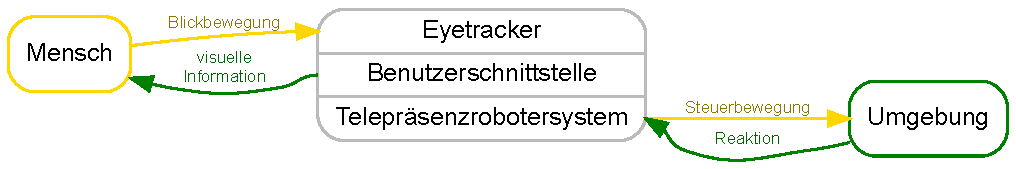
\includegraphics[width=\textwidth]{bilder/grundlagen/simpltrans2.pdf} 
   \end{minipage}% 
\caption{Die Kommunikation zwischen Mensch und Umgebung. Der grundsätzliche Ablauf der Kommunikation ist farblich getrennt hervorgehoben. Mithilfe einer Blickbewegung, die vom Eyetracking-System detektiert wird, kann eine Steuerbewegung des \acl{tps} umgesetzt werden. Die Bewegung kann eine Reaktion der Umgebung erzeugen. Diese Reaktion wird durch das Telepräsenzsystem als Videobild aufgezeichnet und schließlich in Form der visuellen Information über die Benutzerschnittstelle des Systems dem Benutzer zurückgemeldet.}
\label{fig:infotrans}
\end{figure}

Um Strategien zur augenbasierten Steuerung von mobilen Robotersystemen mittels eines Eyetracking-Systems sinnvoll umsetzen zu können, ist es hilfreich, die allgemeine Funktionsweise des menschlichen Auges und seinen Aufbau zu verstehen. Der folgende Abschnitt soll daher zunächst die anatomischen und motorischen Aspekte des Auges darstellen und einführend erklären. Ferner wird auf Erkrankungen mit Bewegungseinschränkungen bei erhaltener Augenbewegung (Okulomotorik) eingegangen und damit eine mögliche Anwendergruppe eingegrenzt. Anschließend werden die in \acs{abb}~\ref{fig:infotrans} skizzierten technischen Komponenten beschrieben. 

\section{Biologische Grundlagen}
\label{section:informationstransfer}
Wie bereits eingangs erwähnt, stellen die Augen bei vielen gravierenden Erkrankungen mit motorischen Beeinträchtigungen oftmals den letzten Kommunikationskanal zur Außenwelt dar. In diesen Situationen kommen ihnen neben rein sensorischen Aufgaben eines Sinnesorgans auch motorische Aufgaben als ausführendes Organ zu. Die Augen nehmen somit eine Art Sonderstellung unter den Sinnesorganen ein und können durch Interpretation der Blickbewegungen zum einen als Indikator für das innere Befinden, das Interesse und die Wünsche eines Menschen dienen und zum anderen als visuelles Eingabesystem für eine grafische Benutzeroberfläche fungieren, ähnlich wie die klassische Computermaus es durch manuelle Eingaben ermöglicht. 

%Um die Blickbewegungen des Benutzers und damit Strategien zur augenbasierte Steuerung von mobilen Robotersystemen zu finden ist es notwendig mit den biologischen Eigenschaften der Augen vertraut zu sein. Der folgende Abschnitt soll daher die anatomischen und motorischen Aspekte des Auges darstellen und einführend erklären.

\subsection{Topografie und Anatomie des Auges}
\label{subsect:topgraf}
Das Auge befindet sich anatomisch in der Augenhöhle (Orbita) des menschlichen Schädels (Cranium) und wird durch mehrere angrenzende Knochenstrukturen stabilisiert und in dieser Position nach dorsal (rückenseits gelegen), medial (zur Mitte hin gelegen) und lateral (zur Seite hin gelegen) geschützt und in seinem Bewegungsumfang begrenzt. Neben dem Augapfel (Bulbus oculi) gehören der Sehnerv (Nervus opticus), die Augenlider, der Tränenapparat und die insgesamt sechs außerhalb des Augenbulbus (extraokulär) angeordneten Augenmuskeln topografisch zum Auge an sich~\cite{Krahn2011}. \acl{abb}~\ref{fig:zugrichtung} zeigt die beschriebenen Strukturen des linken Auges in einer Darstellung von oben. Die Begrenzung des Bulbus nach ventral (bauchseits gelegen) wird vom Ober- und Unterlied (Palpebra superior und inferior) gebildet, in \acs{abb}~\ref{fig:zugrichtung} nicht abgebildet \cite{Krahn2011}. 

\begin{figure}[ht]
   \begin{minipage}[b]{.5\linewidth}          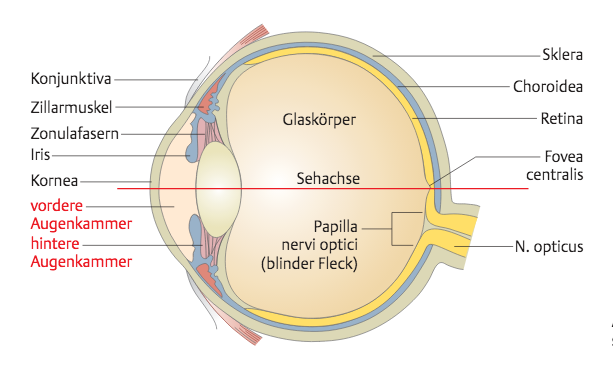
\includegraphics[width=1.05\textwidth]{bilder/grundlagen/g3.png}
      \subcaption{Augapfel (Bulbus oculi)}\label{fig:querschnitt} 
   \end{minipage}% 
   \hfill
   \begin{minipage}[b]{.5\linewidth} 
 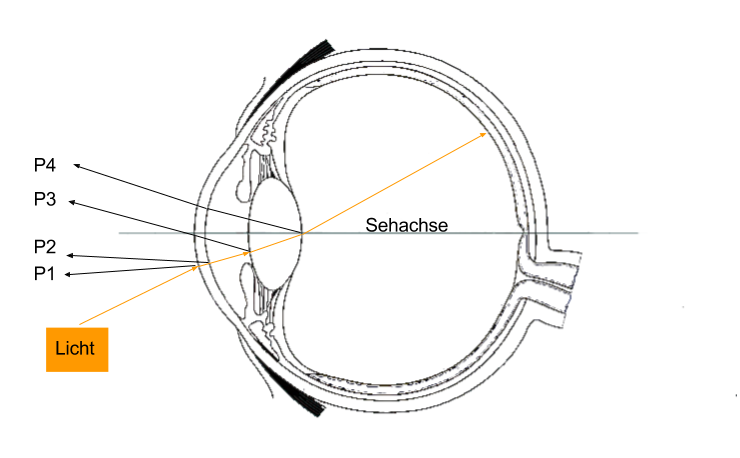
\includegraphics[width=1.05\textwidth]{bilder/grundlagen/g1.png} 
      \subcaption{Purkinje Bilder (P1-P4) }\label{fig:purk}
   \end{minipage}%
   \caption{Das Auges im Längsschnitt mit Darstellung der Anantomie und Lichtreflexion. \textbf{\subref{fig:querschnitt}}~Darstellung der wichtigsten Strukturen des Auges mit den lichtbrechenden Medien; Hornhaut (Cornea), vordere Augenkammer, Linse (Lens cristallina), Glaskörper (Corpus vitreum). \textbf{\subref{fig:purk}}~Entstehung der Lichtreflexionen (Purkinje Bilder) des Auges. Die unterschiedlichen Reflexionen werden nummeriert und mit P1, P2, P3 und P4 bezeichnet. Die Reflexionen resultieren aus der unterschiedlichen Brechkraft der einzelnen Grenzstrukturen im Auge (Vorder- und Rückseite der Cornea, Vorder- und Rückseite der Linse).
(Bild: \textbf{\subref{fig:querschnitt}}~aus \cite[S.438]{Krahn2011},  \textbf{\subref{fig:purk}}~angelehnt an \cite{Krahn2011})}\label{fig:anaauge} 
\end{figure} 

Bei der Betrachtung eines Objektes passiert dessen reflektiertes Licht (elektromagnetische Strahlung mit einer Wellenlänge zwischen 400 und 750 nm) die lichtbrechenden Medien des Auges, siehe \acs{abb}~\ref{fig:anaauge} \cite{Bondke2014}. Jede Struktur hat dabei eine unterschiedliche Brechkraft, die einen Einfluss auf die Gesamtbrechkraft des Auges nimmt. Zu den lichtbrechenden Strukturen zählen somit: (1)~Hornhaut (Cornea), (2)~vordere Augenkammer, (3)~Linse (Lens cristallina) und (4)~Glaskörper (Corpus vitreum).

Die Linse besitzt aufgrund der kollagenhaltigen Zusammensetzung eine Elastizität, die eine Veränderung der Brechkraft ermöglicht, auch bedingt durch den Kontraktionszustand, der innerhalb des Augapfels (intraokulär) gelegenen Muskulatur. Die intraokuläre Muskulatur ist im Rahmen der Nah- und Fernakkommodation aktiv, ferner kann der Lichteinfall durch die Kontraktion und Dilatation der Iris justiert werden. Sobald das Licht die lichtbrechenden Strukturen passiert hat, erscheint das betrachtete Objekt als ein auf dem Kopf stehendes Abbild auf der Netzhaut (Retina) und kann fokussiert werden. Innerhalb der Retina wird die elektromagnetische Strahlung durch lichtempfindliche Rezeptoren (Stäbchen und Zapfen) über ein chemisches Signal in ein elektrisches Signal transferiert und über den Sehnnerv (Nervus opticus, den \RM{2}~Hirnnerv) und die visuelle Nervenbahn in den Hinterhauptslappen des Gehirns (okzipitaler Cortex) geleitet und dort weiterverarbeitet. Durch die Weiterverarbeitung des visuellen Signals entsteht schließlich die visuelle Wahrnehmung und damit die Wahrnehmung der subjektiven Realität des Betrachters. 

\begin{figure}[!ht]
   \begin{minipage}[t]{.5\linewidth} 
      \centering 
      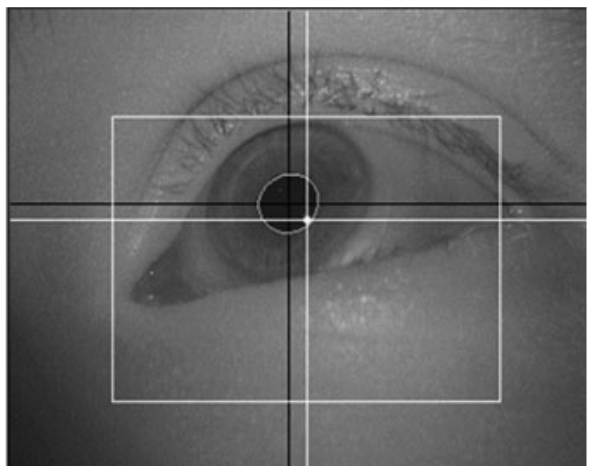
\includegraphics[width=0.94\textwidth]{bilder/grundlagen/Augenreflex.png}
  \subcaption{Corenalreflex des Auges. }\label{fig:purkinje} 
   \end{minipage}% 
   \hfill
   \begin{minipage}[t]{.5\linewidth} 
      \centering 
  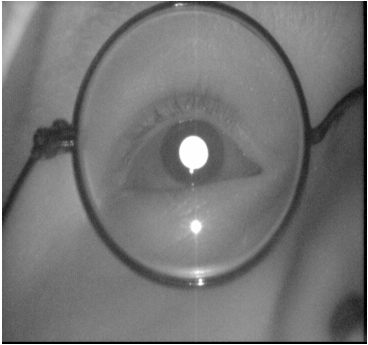
\includegraphics[width=0.8\textwidth]{bilder/grundlagen/reflex.png} 
      \subcaption{Reflexion der Retina.}\label{fig:reflex}
   \end{minipage}%
    \hfill
  \caption{Darstellung ausgewählter Lichtreflexionen des Auges. \textbf{\subref{fig:purkinje}}~Detektion des Corneareflexes und des Pupillenzentrums zur Bestimmung des \acl{por}. \textbf{\subref{fig:reflex}}~Reflexion der Retina. Die Lichtquelle strahlt koaxial zur optischen Achse des Auges, wobei die Netzhaut einen Großteil des Lichtes reflektiert. Dieser Effekt entspricht dem in der Fotografie bekannten Rote-Augen-Effekt. (Bild: \textbf{\subref{fig:purkinje}} aus \cite{Majaranta2014}, \textbf{\subref{fig:reflex}} aus \cite[Abb. 3]{Joos2003})}\label{fig:reflexpurkije} 
\end{figure} 

Bei diesem eben geschilderten Verlauf der Lichtstrahlung wird ein Teil des Lichtes an den beschriebenen lichtbrechenden Strukturen reflektiert und am Auge sichtbar, \vgl \acs{abb}~\ref{fig:purk} und \acs{abb}~\ref{fig:reflexpurkije}. Diese Reflektionen werden als \textit{Purkinje-Bilder} bezeichnet und aufgrund der unterschiedlich reflektierenden Strukturen unterschieden. Das erste Purkinje-Bild entsteht durch die Reflektion an der Außenseite der Cornea (P1), das zweite (P2) durch die Reflexion an der Innenseite der Cornea und das dritte (P3) an der Vorderfläche der Linse. (P4) wird schließlich durch die Grenzfläche an der Rückseite der Linse erzeugt. \acl{abb}~\ref{fig:purk} veranschaulicht das eben Beschriebene. Ein weiteres Phänomen ist die Reflexion der Retina bei einer koaxialen Beleuchtung in Bezug zur optischen Achse des Auges. Siehe \acs{abb}~\ref{fig:reflex} \cite{Joos2003,Eidam2015}. Sowohl die Purkinje-Bilder als auch die Cornealreflektion werden durch Eyetracking-Systeme verwendet, siehe Abschnitt~\ref{section:eyeMet}. 



\subsection{Okulomotorik des Auges}
\label{subsection:okumot}
Die extraokulär angeordnete Muskulatur ist für die Augenbewegungen (Okulomotorik) verantwortlich, siehe \acs{abb}~\ref{fig:zugrichtung}. Grundsätzlich lassen sich durch die Anordnung der extraokulären Muskulatur, die in \acs{abb}~\ref{fig:augenbewegung} dargestellten, drei aufeinander senkrecht stehenden Bewegungsachsen unterscheiden. Der Schnittpunkt dieser Achsen bildet das Drehzentrum des Auges, wodurch folgende willkürliche Bewegungen entlang der genannten Achsen ausgeführt werden können ~\cite{Thoemke2008,Bondke2014}. 

\begin{enumerate}
\item  Abduktions-/Adduktionsbewegungen entlang der vertikalen Achse, die durch den M. rectus medialis und M. rectus lateralis erfolgen, \vgl \acs{abb}~\ref{fig:zugrichtung}. Werden Ab\-duktions- und Ad\-duktionsbewegungen alternierend ausgeführt, entsteht hieraus eine horizontale Augenbewegung. 
\item Elevations-/Depressionsbewegungen entlang der horizontalen Achse, die durch den M. rectus superior und den M. rectus inferior erfolgen,  \vgl \acs{abb}~\ref{fig:zugrichtung}. Werden Elevations,- und Depressionsbewegungen alternierend ausgeführt, entsteht hieraus eine vertikale Augenbewegung.
\item Ex-/Intorsionsbewegungen, also Außen-/Innenrotationsbewegungen entlang der optischen Achse, die durch den M. obliquus superior und M. obliquus inferior erfolgen, \vgl \acs{abb}~\ref{fig:zugrichtung}. Alternierende Bewegungen beider Muskeln in Kombination mit dem \og M. rectus superior und dem M. rectus inferior führen zu diagonalen Augen- oder zu Rotationsbewegungen im Rahmen von Kopfschiefhaltungen.
\end{enumerate}

\begin{figure}[ht]
   \begin{minipage}[t]{.5\linewidth} 
      \centering 
    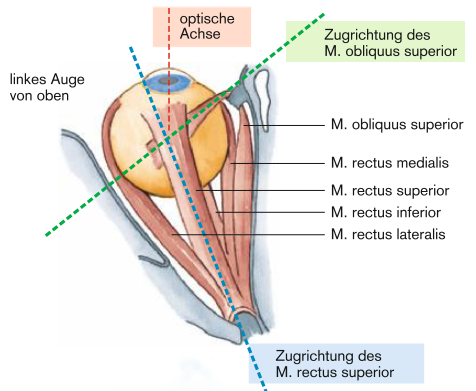
\includegraphics[width=1\textwidth]{bilder/grundlagen/g5.png}
  \subcaption{Linkes Auge von oben}\label{fig:zugrichtung} 
   \end{minipage}% 
   \hfill
 	\begin{minipage}[t]{.5\linewidth} 
      \centering 
   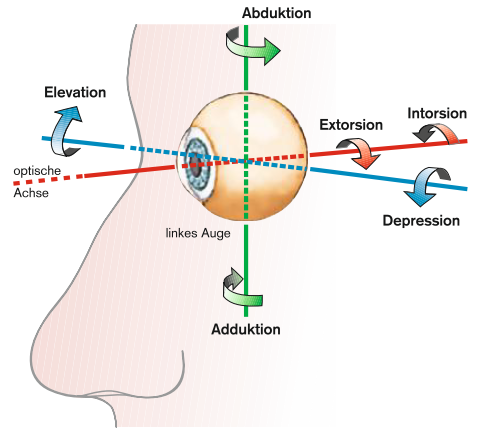
\includegraphics[width=0.9\textwidth]{bilder/grundlagen/g4.png} 
  \subcaption{3 Bewegungsachsen der Augen }\label{fig:augenbewegung} 
   \end{minipage}%
   \caption{Zugrichtung der Augenmuskulatur und Bewegungsachsen. \textbf{\subref{fig:zugrichtung}}~Periokuläre Augenmuskulatur mit fünf der sechs Augenmuskeln. Farblich hervorgehoben ist die Zugrichtung des M. obliquus superior (grün) und des M. rectus superior (blau).  \textbf{\subref{fig:augenbewegung}}~Die drei Bewegungsachsen der Augen mit farblicher Unterscheidung der Abduktions-/Adduktionsbewegungen (grün), Elevations-/Depressionsbewegungen (blau), Ex-/Intorsionsbewegungen (rot). (Bild: aus \textbf{\subref{fig:zugrichtung}}~\cite[S.777]{Bondke2014}, \textbf{\subref{fig:augenbewegung}}~\cite[S.776]{Bondke2014})}\label{fig:augbilder} 
\end{figure} 

Die genannten Bewegungen können willkürlich ausgeführt werden und dienen teilweise als Augengesten im Rahmen der Interaktion mit der implementierten Benutzerschnittstelle.
Eine weitere Bewegung, die für die aktuelle Arbeit von Bedeutung ist, ist die des Lidapparates (Ober- und Unterlied). Der Lidschluss erfolgt durch den in \acs{abb}~\ref{fig:augbilder} nicht dargestellten M. orbicularis oculi~\cite{Krahn2011}. Die Lidöffnung durch den M. levator palpebrae superior, ebenfalls in \acs{abb}~\ref{fig:augbilder} nicht mit abgebildet~\cite{Krahn2011}.

Neben der muskulären Anordnung ist für die Durchführung einer Augenbewegung die nervale Innervation entscheidend. Die sechs Augenmuskeln werden von insgesamt drei Hirnnerven versorgt, die ihren Ursprung in den jeweiligen Hirnnervenkernen im Hirnstamm haben. Somit ist die Ausführung einer regelrechten Augenbewegung maßgeblich von einem intakten Hirnstamm abhängig. Die Versorgung des für die Abduktion zuständigen Augenmuskeln M. rectus lateralis erfolgt über den \RM{6}~Hirnnerv (Nervus abducens). Verletzungen des Muskels oder der nervalen Innervation führen zu einer Störung der Bewegung im Rahmen der horizontalen Augenbewegung. Die Außenrotation (Extorsion) wird über den \RM{4}~Hirnnerv (N. trochlearis) vermittelt und beeinträchtigt die diagonale Blickbewegungen. Darüber hinaus führt die Schädigung des Muskels oder der nervalen Strukturen zu einer Kopfschieflage, um damit die resultierenden Doppelbildern zu kompensieren. Die restlichen Muskeln (M. rectus superior, inferior, medialis; M. obliquus inferior) werden vom \RM{3}~Hirnnerv (N. oculomotorius) innerviert \cite{Bondke2014}. Die Motorik des Lidapparates wird für die Lidöffung vom \RM{3}~Hirnnerv (N. oculomotorius) vermittelt, der Lidschluss durch den N. facialis (\RM{7}~Hirnnerv)~\cite{Krahn2011}.

Zusätzlich zu diesen \og Bewegungen der Augenbuli lassen sich noch Bewegungsformen der visuellen Orientierung und Wahrnehmung unterscheiden~\cite{Bondke2014}, die im Bereich der Detektion von Augengesten von Bedeutung sind. Ziel dieser Blickbewegungen im Rahmen der visuellen Wahrnehmung ist es, den Ort des schärfsten Sehens (Fovea centralis) immer wieder durch schnelle Augenbewegungen auf ausgewählte Fixationspunkte auszurichten, um diese Punkte dadurch zu fokussieren~\cite{Bondke2014}. Die Augenmuskulatur zeichnet sich durch kleine motorische Einheiten (Neuron und Muskelfasern) mit ca. 5 - 10 Muskelfasern pro Motoneuron~\cite{Bondke2014} aus. Im Vergleich zu großen Muskelgruppen im Bereich der unteren oder oberen Extremitäten mit 100 - 1000 Muskelfasern pro Motoneuron. Erst dadurch werden feine und schnelle Bewegungen der Augen ermöglicht. Folgende Bewegungen werde unterschieden und sind aus~\cite{Bondke2014,Thoemke2008,Joos2003} zusammengetragen:

\begin{description}
\item[Fixation] Bezeichnet die Bewegung, die das Fixationsobjekt auf den Ort des schärfsten Sehens abbildet. Während der Fixation finden zur Stabilisierung des Bildes Mikrobewegungen statt. Als Beispiel dient \acs{abb}~\ref{fig:sakkad}.
\item[Sakkaden] Während eines Blickwechsels von einem Objekt zum anderen werden die Augen durch schnelle Augenbewegungen, die sogenannten Sakkaden, zum nächsten Fixationsziel bewegt. Sakkaden gehören zu den schnellsten Muskelbewegungen, die Menschen ausführen können (Winkelgeschwindigkeit bis $ 700 \,^\circ/s $) \cite{Bondke2014}. Für genauere Ausführungen zur Beziehung zwischen Sakkadenamplitude und Sakkadengeschwindigkeit sei auf \cite[S.12 ff.]{Thoemke2008} verwiesen. Zur Verdeutlichung von Sakkaden dient auch hier \acs{abb}~\ref{fig:sakkad}.
\item[Folgebewegung] Befindet sich das fixierte Objekt in Bewegung, werden langsame Bewegungen ausgeführt, um trotz der relativen Bewegung des Objektes eine scharfe und präzise Abbildung auf der Fovea zu erzeugen. Diese Bewegungen erreichen Winkelgeschwindigkeiten bis zu $100 \,^\circ/s$ \cite[S.30]{Thoemke2008}.
\item[Mikrobewegungen] Hierzu zählen Drift, Tremor und Mikrosakkaden, die, wie oben genannt, während der Fixation auftreten. Zum Drift kommt es aufgrund der physiologischen Eigenschaften der Nervenzellen in der Retina, die primär auf Veränderung ausgelegt sind und zur Aufrechterhaltung der Stimulation minimal verändert werden. Diese Driftbewegung wird durch Mikrosakkaden ausgeglichen. Der Tremor wird durch Ungenauigkeiten in der Muskelsteuerung hervorgerufen.
\item[Vergenzbewegungen] Darunter versteht man Ausgleichsbewegungen, die das Auftreten von Doppelbildern bei sich nähernden oder entfernenden Zielobjekten vermeiden. 
\end{description}

\subsection{Erkrankungen mit erhaltener Okulomotorik}
\label{subsect:erkrank}
Im Rahmen der vorliegenden Arbeit soll die Okulomotorik zur visuellen Mensch-Computer-Interaktion i. S. einer Steuerung eines mobilen Robotersystems genutzt werden. Anwendungsgruppen sind Personen mit Sprach- und Bewegungseinschränkungen. Wie bereits im Abschnitt~\ref{subsection:okumot} beschrieben, sind die nervalen Strukturen im Hirnstamm sowie die muskulären Effektoren am Auge entscheidend für eine adäquate Augenkoordination und somit für einen problemlosen Informationstransfer zwischen Mensch und Computer. Dieser Abschnitt benennt mögliche Krankheitsbilder mit erhaltener Okulomotorik bei subtotaler oder totaler Bewegungseinschränkung.

%%%%%%%%%%%%%%%%%%%%%%%%%%%%%%%%%%%%%%%%%%%%%%%%%%%%%%%%%%%%%%%%%%%%%%%%%%%%
%-VENI-VENI-VENI-VENI-VENI-VENI-VENI-VENI-VENI-VENI-VENI-VENI-VENI-VENI-VENI
%-VENI-VENI-VENI-VENI-VENI-VENI-VENI-VENI-VENI-VENI-VENI-VENI-VENI-VENI-VENI

\begin{description}
\item[ALS] Die \acs{als} ist eine Motoneuron-Erkrankung, die mit dem Verlust der motorischen Bewegungen einhergehen kann und bislang nicht heilbar ist. Die Augenkerne im Hirnstamm werden in aller Regel erst spät im Krankheitsverlauf beeinträchtigt, sodass diese als Kommunikationskanal genutzt werden können. Im Spätstadium ist jedoch auch ein kognitiver Abbau bekannt und eine erhöhte Komplikationsrate,- beispielsweise durch eine Atemersatztherapie.
\item[Hoher Querschnitt (traumatisch, demyelinisierend, entzündlich, neoplastisch)] Ein hoher Quer\-schnitt kann traumatisch bedingt, also durch Verletzungen der Halswirbelsäule auf Höhe der Halswirbelkörper C3-C5 verursacht werden, welcher mit einer Muskelschwäche bis hin zur Muskellähmung aller vier Extremitäten (Tetraparese oder Tetraplegie) und damit verbundener Immobilität einhergehen kann~\cite{VanMiddendorp2014a}. Des Weiteren kann ein hoher Querschnitt durch demyelinisierende Erkrankungen (\zB Multiple Sklerose), neoplastische Raumforderung (spinale Tumoren) oder durch Entzündungen (Hirnstammencephalitis, Abszess) mit Veränderungen des Rückenmarkes auf cervikaler Ebene hervorgerufen werden.
\item[Hypoxischer Hirnschaden] Dies ist eine Schädigung des Gehirns, die durch verschiedenen Erkrankungen/Unfälle infolge von Sauerstoffminderversorgung des Gehirns entstanden ist. Diese Form kann sich verschieden klinisch manifestieren und ist abhängig von der Schädigungslokalisation im Gehirn. 
\item[Schlaganfälle] (Ischämie oder Blutung): Ein Schlaganfall entsteht zum Großteil entweder durch eine Gefäßthrombose und damit einhergehende Sauerstoffminderversorgung der betroffenen Gehirnareale oder durch eine Blutung und damit verbundenem Zelluntergang und Schädigung des Gehirns. 
\item[\acf{lis}] Das \acs{lis} wird durch eine bilaterale Schädigung der ventralen Pons (Brücke) des Hirnstamms verursacht, die zu einer Tetraplegie und Anarthrie (Ausfall der Sprechfunktion) bei erhaltenem Bewusstsein führt~\cite{Khanna201196}. Ursachen können zum einen Durchblutungsstörungen der Arteria basilaris, die für die Blutversorgung des Hirnstamms zuständig ist, sein, zum anderen Blutungen und Entzündungen des Hirnstamms. Für ein~\acs{lis} können ebenso Tumore im Hirnstamms oder eine pontine Myelinolyse ursächlich sein, welche durch zu rasche Korrektur des initial erniedrigten Blutnatriumspiegels zu einer Schädigung der Pons führt~\cite{steven2005}. Nach Bauer et al. (1979)~\cite{Bauer1979} wird das \acs{lis} durch den Grad der motorischer Beeinträchtigung unterteilt in (a)~\textit{klassisches LIS}, das dadurch charakterisiert wird, dass eine komplette Immobilität vorherrscht, jedoch sowohl die vertikale Augenbewegung als auch die Augenlidbewegung möglich ist. (b)~\textit{inkomplettes LIS} erlaubt willkürliche Bewegungen und (c)~\textit{totales LIS} beinhaltet die komplette Immobilität auch der Augenbewegungen bei erhaltener Bewusstseinslage~\cite{Khanna201196}.
\end{description}

Nachfolgend wird als nächste Komponente im Rahmen einer Kommunikation zwischen Mensch und Umwelt auf Eyetracking-Systeme eingegangen.

\section{Eyetracking-Systeme}
\label{section:eyetracker}

Nach der ausführlichen Beschreibung der Okulomotorik und der anatomischen Eigenschaften der Augen soll der folgende Abschnitt das technische Hilfsmittel zur Detektion und Nutzung von Blick- und Augenbewegungen den Eyetracker einleitend vorstellen. Dabei wird ein Überblick über die Eyetracking-Methoden gegeben. Ferner wird der spezielle Nutzen von Eyetracking-Systemen als Eingabegerät zur Steuerung einer Benutzerschnittstelle beschrieben. Dieses Kapitel orientiert sich inhaltlich an den Ausführungen von Majaranta und Bulling (2014), sowie an Lupu (2013) und Hollomon et al. (2017)~\cite{Lupu2013,Majaranta2014,Hollomon2017}. 

\subsection{Eyetracking-Methoden}
\label{section:eyeMet}
Eyetracking-Systeme haben sich initial aus dem Wunsch der Menschen entwickelt, Einblicke in die Physiologie der Augenbewegung zu erhalten, um den visuellen Apparat als Sinnesorgan genauer zu verstehen. Die Entwicklung von Methoden zur Aufzeichnung von Augenbewegungen gehen auf das Jahr 1879 zurück, als Emile Java, ein französischer Augenarzt, Selbstversuche während des Lesens mithilfe eines einfachen Spiegels aufzeichnete~\cite{Lupu2013}. Eyetracking-Systeme haben sich seitdem durch den technischen Fortschritt weiterentwickelt und befinden sich seit mehreren Jahrzehnten, beispielsweise in der psychologischen und neurowissenschaftlichen Forschung, als diagnostisches Werkzeug zur Erforschung kognitiver Prozesse und Intentionen der Benutzer im Einsatz~\cite{Duchowski2002}.

Allgemein bezeichnet Eyetracking eine Methode, die es ermöglicht, die Augenbewegungen eines Anwenders zu erfassen und daraus auf seinen aktuellen Betrachtungspunkt zu schließen. Der Betrachtungspunkt wird auch als sogenannter \acf{por} bezeichnet. Damit können die genaue Blickbewegung und -position des Anwenders während der Nutzung in Relation zu unterschiedlich präsentierten Stimuli untersucht werden~\cite{SMI2011}. \acl{abb}~\ref{fig:sakkad} zeigt die durch ein Eyetracking-System aufgezeichneten und farblich hervorgerufenen Blickpositionen beim Lesen eines Textes. Die Darstellung veranschaulicht die bereits in Abschnitt~\ref{subsection:okumot} charakterisierten Augenbewegungen, die durch die Nutzung eines Eyetracking-Systems sichtbar werden. 
 
\begin{figure}[ht]
   \begin{minipage}[b]{\linewidth} 
      \centering 
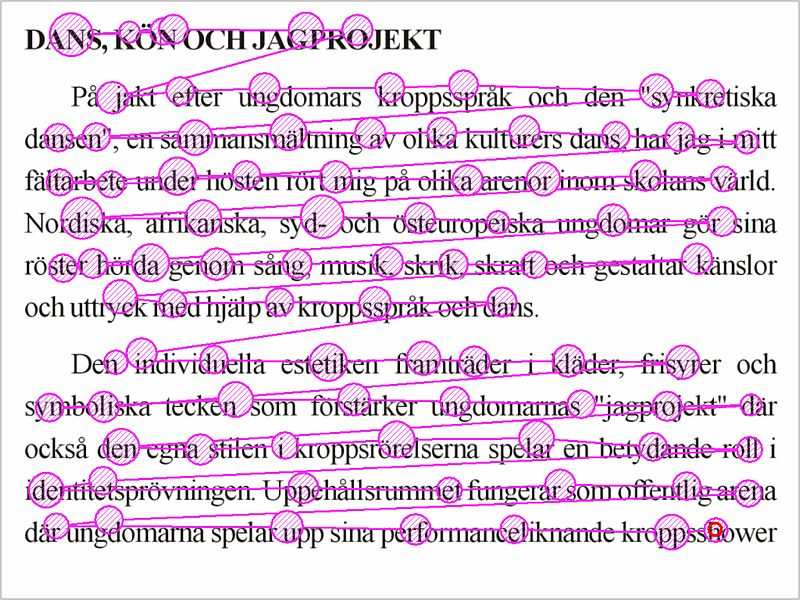
\includegraphics[scale=3]{bilder/grundlagen/sakkaden.jpg}
   \end{minipage}% 
   \hfill
   \caption{Fixation und Sakkaden während des Lesens (schwedischer Text). Aufzeichnung eines videobasierten Eyetracking-Systems der Firma \acs{smi} während eines Schnelllese-Wettbewerbs. Zu Erkennen, sind die als runde Punkte dargestellte Fixierungen, getrennt durch schnellen Sakkadenbewegung. (Bild: aus \url{https://commons.wikimedia.org/wiki/File:Reading_Fixations_Saccades.jpg} letzter Aufruf: 6. Februar 2017)}\label{fig:sakkad} 
\end{figure}

Die Methodik der Detektion hat sich initial von invasiven Verfahren hin zu aktuell weitgehend noninvasiven Techniken weiterentwickelt~\cite{Joos2003,Lupu2013}. Nachfolgend werden einige ausgewählte Verfahren beschrieben, die zur Detektion von Augenbewegungen verwendet werden.  Für weitere Methoden sei auf Joos et al. (2003) und Young und Sheena (1975) verwiesen~\cite{Joos2003, Young1975}.

\begin{description}
\item[Elektrookulografie] Dieses Verfahren mittels \acs{eog} macht sich die natürliche elektrische Potenzialdifferenz zwischen der Vorder- und Hinterseite des Augenbulbus zur Detektion der Augenbewegung zunutze, \vgl \acs{abb}~\ref{fig:pmsub1}. Die Potenzialdifferenz entsteht durch einen negativen Pol am Augenfundus und einem positiven Pol an der Hornhaut~\cite{Lupu2013,Barea2002}. Dabei ist die Potenzialdifferenz mit einer Spannung von 0.4 bis 1.0 mV ausreichend, um diese mittels fünf periorikulär angebrachten Elektroden zu messen, siehe \acs{abb}~\ref{fig:pmsub2} \cite{Lupu2013}. Erfolgt eine gerichtete Augenbewegung, entsteht durch die Richtung der Bewegung ein unterschiedlicher Spannungsverlauf zwischen den angebrachten Elektroden. Für eine genauere Ausführung sei auf \cite{Joos2003} verwiesen. Die Detektion der Augenbewegung beruht auf dem Verhältnis zwischen Blickwinkel~$\sigma$ und der Spannung~$U$, wobei die Spannungsdifferenz bis zu einem Blickwinkel von $40\,^\circ$ annähernd proportional ist: $U_0 = U_0 * sin \sigma$ \cite{Joos2003}. 

\begin{figure}[ht]
   \begin{minipage}[b]{0.5\linewidth} 
      \centering 
  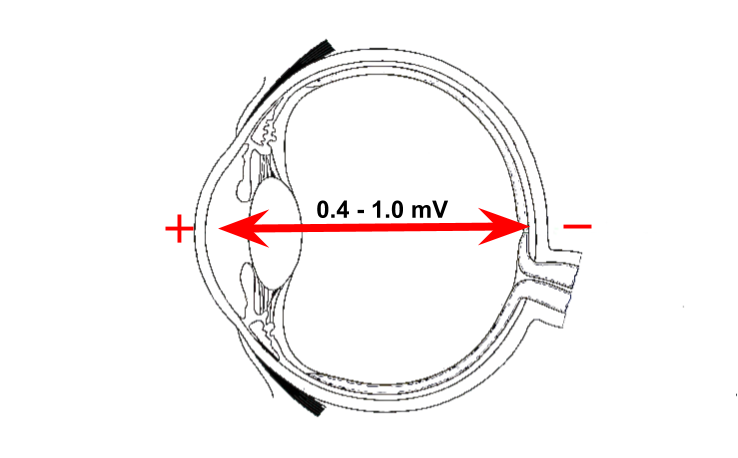
\includegraphics[width=1\textwidth]{bilder/grundlagen/plusminus.png}
    \subcaption{Potenzialdifferenz des Auges}\label{fig:pmsub1}
   \end{minipage}% 
   \hfill
   \begin{minipage}[b]{0.5\linewidth} 
      \centering 
  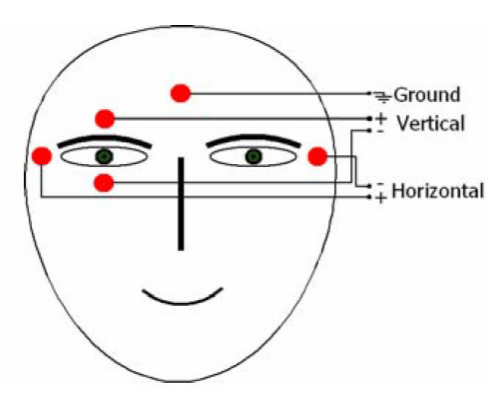
\includegraphics[width=0.8\textwidth]{bilder/grundlagen/eog.png}
  \subcaption{periokuläre Elektroden}\label{fig:pmsub2}
   \end{minipage}% 
   \hfill
   \caption{\acf{eog} mit der Positionierung der Elektronen. (Bild: \subref{fig:pmsub1}und \subref{fig:pmsub2} angepasst aus \cite[S.74]{Lupu2013})}\label{fig:plusminus} 
\end{figure} 

\item[\enquote{Bright Pupil}-Verfahren] Es basiert auf einem Algorithmus, der sich die Reflexion der Cornea, also das Purkinje-Bild (P1) und das Pupillenzentrum zur Bestimmung des \acs{por} zunutze macht. Als Lichtquelle wird ein Infrarotlicht verwendet, wodurch der Benutzer im Vergleich zum sichtbaren Licht nicht geblendet wird. Durch die Positionierung der Lichtquelle eng an der optischen Achse des Auges erfolgt eine Lichtreflexion durch die Netzhaut. Die Pupille erscheint hell (bright) und lässt sich mittels einer zum System gehörenden Kamera aufzeichnen. Aus dem Videobild werden unter Zuhilfenahme von Bilderkennungsalgorithmen das Pupillenzentrum und der Cornealreflex detektiert. Der resultierende Vektor der beiden Punkte, der sich in Abhängigkeit der Blickposition verändert, lässt letztlich auf den \acs{por} des Benutzers schließen \cite{Poole2005}. \acl{abb}~\ref{fig:schemaPurk} verdeutlicht diese Beschreibung und zeigt die helle Pupille und den Cornealreflex schematisch aus Sicht der Kamera. Der Cornealreflex verändert sich in Relation zum Pupillenzentrum in Abhänigkeit der Blickposition.
\item[\enquote{Dark Pupil}-Verfahren] Diese Methode basiert,- auf denselben Prinzipien wie das Bright-Pupil-Verfahren. Die Pupille wird jedoch in einem anderen Winkel beleuchtet und erscheint aus diesem Grund dunkel (dark). Das Bright-Pupil-Verfahren und das Dark-Pupil-Verfahren zählen zur Gruppe der videobasierten Eyetracking-Methoden. Die vorliegende Arbeit basiert auf dem letzterem Prinzip.

\begin{figure}[ht]
\begin{minipage}[t]{\linewidth} 
      \centering 
      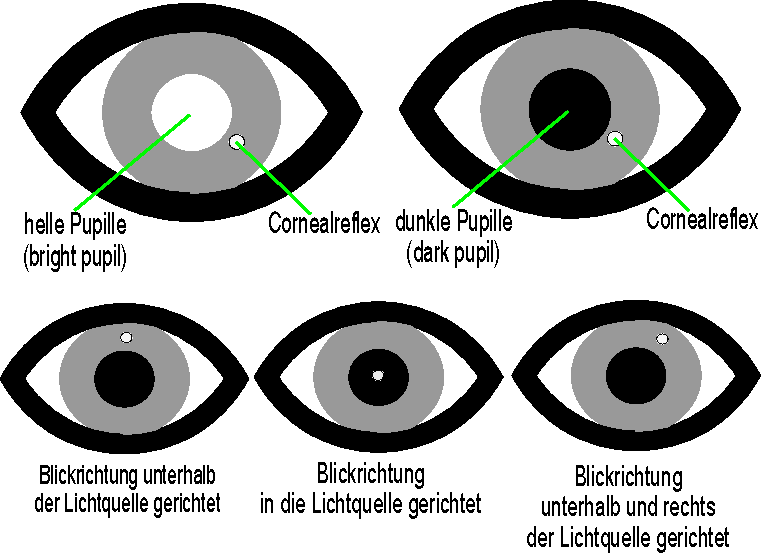
\includegraphics[scale=0.7]{bilder/grundlagen/eye22.pdf}
  \caption{Schematische Darstellung eines Auges mit unterschiedlicher Abbildung Bright- \bzw Dark-pupil Verfahrens (oben). Veränderung des Cornealreflexes in Abhängigkeit der Blickbewegung (unten). (Darstellung angelehnt an Pool et al.~\cite{Poole2005}).}\label{fig:schemaPurk} 
   \end{minipage}% 
\end{figure}
\end{description}

Eyetracking-Systeme ermöglichen neben der Erfassung des \acs{por} die Bestimmung weiterer Parameter,- wie \zB die Erfassung des Pupillendurchmessers, des Lidschlusses, der Anzahl der Fixationen an einem bestimmten Punkt, oder der Dauer der Fixationen an unterschiedlichen Punkten \cite{Joos2003,Jacob2003, Poole2005}. Ferner lassen Parameter wie der sogenannte Scan-Path, also die Folge des Fixationsverlaufs oder der Bereich des Blickfeldes, der besonders häufig beobachtet wird (Area of interest), Rückschlüsse auf das Interesse des Nutzers \cite{Jacob2003,Lupu2013, Peters2013} zu. Für die vorliegende Arbeit stehen die Erfassung der Blickbewegung \bzw der Fixation, der horizontalen und vertikalen Augengeste und die Erkennung des Lidschlusses im Vordergrund.

Nachfolgend werden einige Eigenschaften des für die vorliegende Arbeit verwendeten videobasierten Eyetracking-Systems beschrieben.

\subsection{Eigenschaften videobasierter Eyetracking-Systeme}
\label{section:vidMet}
Videobasierte Eyetracking-Systeme werden heutzutage unter den verwendeten Eyetracking-Systemen häufig verwendet \cite{Poole2005,SMI2011}. Vorteile dieser Systeme liegen in der wenig invasiven Technik und der robusten Augen\-detektion \cite{SMI2011}. 
Diese Systeme lassen sich zusätzlich zur Detektionsmethode durch den Befestigungsort des \textit{\aclp{et}~(ETM)} unterscheiden. Damit ist die Komponente gemeint, die meistens sowohl die Infrarot-Lichtquelle,- als auch die aufzeichnende Kamera enthält. Bei mobilen \textit{\acl{hed}} Systemen ist die Kamera an einem Brillengestell oder einer Helmvorrichtung angebracht, siehe \acs{abb}~\ref{fig:eyeTrackingsub1}. Auf eine Positionierung des Eyetrackingmoduls am Kopf des Anwenders verzichten \textit{stationäre Eyetracking-Systeme}, siehe \acs{abb}~\ref{fig:eyeTrackingsub2}.

\begin{figure}[ht]
   \begin{minipage}[t]{0.5\linewidth} 
      \centering 
      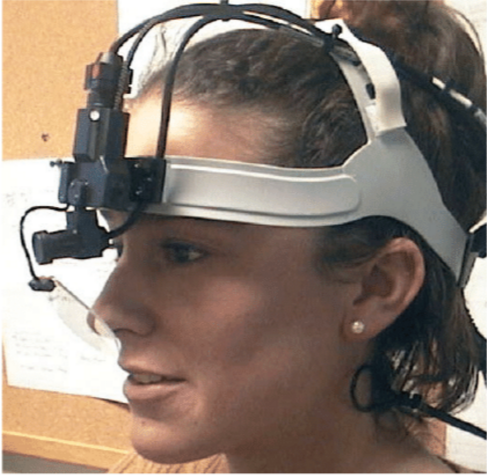
\includegraphics[width=.7\textwidth]{bilder/grundlagen/HDM.png}
     \subcaption{\acl{hed}}\label{fig:eyeTrackingsub1}
   \end{minipage}% 
   \hfill
   \begin{minipage}[t]{0.5\linewidth} 
      \centering 
      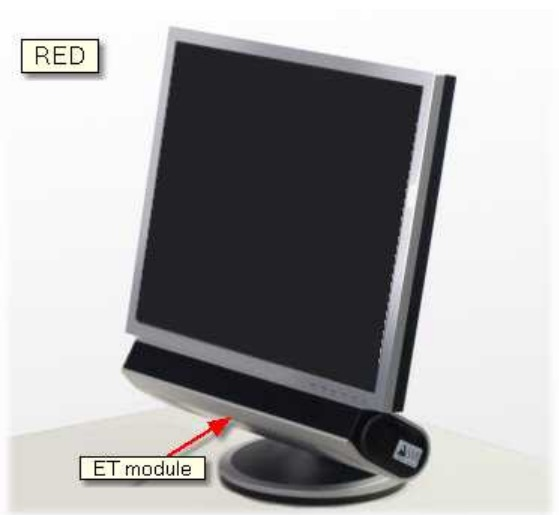
\includegraphics[width=0.8\textwidth]{bilder/implementierung/Eye3.JPG}
   \subcaption{stationäre Eyetracker }\label{fig:eyeTrackingsub2}
   \end{minipage}% 
    \hfill
   \caption{Darstellung zweier videobasierter Eyetracking-Systeme. (Bild: \textbf{\subref{fig:eyeTrackingsub1}}~\cite{Goldberg2003}, \textbf{\subref{fig:eyeTrackingsub2}}~\cite[S.136]{SMI2011})}\label{fig:device} 
\end{figure} 

Die vorliegende Arbeit verwendete das stationäre System \acf{red} der Firma \acf{smi}, das in \acs{abb}~\ref{fig:eyeTrackingsub2} dargestellt ist. \acl{abb}~\ref{fig:eyeTrackingsub2} zeigt die typische Positionierung des \acs{et} mit Kamera und Infrarot- Lichtquelle unter oder neben dem stimuluspräsentierenden Monitor. Die Position lässt sich jedoch auch variieren.  Das in \acs{abb}~\ref{fig:eyeTrackingsub2} gezeigte \acs{et} ist aufgrund zweier Infrarot-Lichtquellen auch für eine binokularen Nutzung ausgelegt \cite{Eidam2015,SMI2011}. Damit ist prinzipiell eine getrennte Detektion der Augenbewegungen der Augenpaare möglich. Standardmäßig gehört gewöhnlich auch eine Computereinheit, die die oben erwähnten bildverarbeitende Algorithmen zur Berechnung des \acs{por} ausführt, zu den Komponenten eines videobasierten Systems. 

Bei stationären Systemen wie dem \acs{red}-System ist eine bestimmte Positionierung der Versuchsperson und der Augenposition zur Optimierung des Detektionsergebnisses wichtig. Die schematische Darstellung des Herstellers in \acs{abb}~\ref{fig:empfehlung} verdeutlicht die empfohlene Anordnung. Er empfiehlt bei der Durchführung eine Entfernung von 60 - 80 cm vom \acs{et} einzuhalten.

\begin{figure}[ht]
\begin{center}
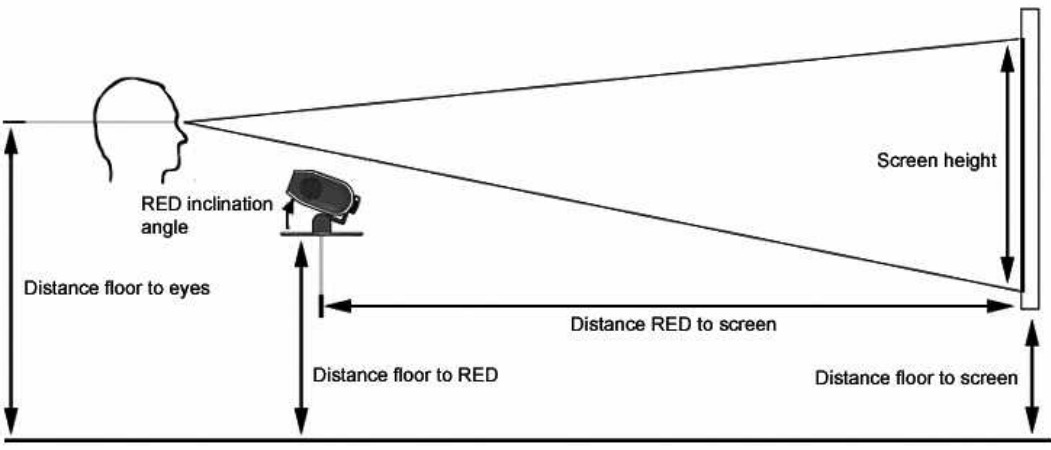
\includegraphics[width=0.7\textwidth]{bilder/grundlagen/Schema.JPG}
\end{center}
\caption{Schema der empfohlenen Anordnung.
Die Positionierung des \acs{et} im Verhältnis zur Kopfposition. (Bild: aus \cite[S.150]{SMI2011})}
\label{fig:empfehlung}
\end{figure}

Ferner ist zur präzisen Berechnung des \acs{por} eine Kalibrierung für videobasierte Eyetracking-Systeme individuell für jeden Anwender im Vorfeld der Nutzung notwendig. Dabei ist auch eine Instruktion des Anwenders vor Beginn der Benutzung sinnvoll. Bei der Kalibrierung werden definierte Punkte am Bildschirm angezeigt, während vom System die entsprechenden Pupillenpositionen in Abhängigkeit der Bildschirmkoordinaten erfasst und intern zur Optimierung des \acs{por} verwendet werden.  

Weitere Faktoren, die die Qualität der Detektion der Augenposition reduzieren können, sind neben der Kopf- \bzw Augenpositionierung,- schlechte Lichtverhältnisse, Brillengläser, tief hängende Augenlieder oder auch Make-up. Ferner können durch Kopfbewegungen Fehlinterpretationen seitens des Systems entstehen, auch wenn diese intern teilweise kompensiert werden können \cite{SMI2011}.

Nach den eben beschriebenen Eigenschaften und dem Aufbau videobasierter Eyetracking-Systeme, sowie der Methodik zur Detektion von Augengesten ist im Weiteren die damit verbundene Interaktion mit einer grafischen Benutzerschnittstelle relevant. 

\subsection{Augengesten als Eingabemechanismus für grafische Benutzer\-ober\-flächen}
\label{subsection:eingabemech}

Die Anwendungsmöglichkeiten eines Eyetracking-Systems reichen von der Funktion als passive Informationsquelle, beispielsweise in der Forschung, bis hin zu einem aktiven Eingabemechanismus,- \zB während der Bedienung einer grafischen Benutzeroberfläche \cite{majaranta2011,Majaranta2014}. Während einerseits die Augenbewegungen eher im Hintergrund aufgezeichnet werden und damit keine speziellen Anforderungen an den Benutzer gestellt werden, finden andererseits willkürlich kontrollierte Augenbewegungen als Steuersignale für ein Computersystem Anwendung und somit werden Anforderungen an die kognitiven Fähigkeiten des Benutzer gestellt \cite{majaranta2011,Majaranta2014}. 

Trotz dieser Anforderungen bieten Eyetracking-Systeme als Eingabemedium zur Interaktion mit einer grafischen Benutzeroberfläche Einsatzmöglichkeiten speziell für Menschen mit motorischen Beeinträchtigungen \cite{Majaranta2014,Eidam2015,Eidam2016}. 

Der in der vorliegende Arbeit verwendete Prototyp dient ausschließlich als Eingabegerät zur Interaktion mit einer grafischen Benutzeroberfläche und nutzt explizit definierte Augengesten als aktive Steuersignale zur Bedienung eines mobilen Robotersystems. 

Um mit Elementen einer grafischen Benutzeroberfläche wie \zB mit Knöpfen (Buttons) und mit kleinen Symbolgrafiken (Icons) zu interagieren, müssen vom Eingabegerät hauptsächlich Zeige- und Selektionsoptionen bereitgestellt werden. Die Computermaus als klassisches manuelles Eingabegerät erfüllt diese Funktion durch die Repräsentation der eigenen relativen Position als eine abstrakte Zeiger- \bzw Fingerposition auf dem Bildschirm \cite{Peters2013}. Der Benutzer kann durch Positionierung des Mauszeigers auf Elemente der grafischen Benutzerschnittstelle einfache Zeigehandlungen ausführen. Durch das Betätigen der Maustasten (klicken) kann ein Element gezielt selektiert werden. Mit einer Computermaus sind darüber hinaus noch \textit{Drag-And-Drop}- Operationen möglich \cite{Peters2013}; also die Interaktion mit ausgewählten Elementen der Benutzeroberfläche in Form eines Verschiebens und Loslassens dieser Elemente.

Um mithilfe eines Eyetracking-Systems zumindest Zeige- und Selektionsoperationen realisieren zu können, sind die in Abschnitt~\ref{subsection:okumot} genannten Augenbewegungen relevant, die als Steuerkommandos verwendet werden können. In der Literatur wurden unterschiedliche Blick- und Augengesten im Hinblick auf ihre Nützlichkeit und Effizienz als Eingabesignal untersucht, \vgl~\cite{Hollomon2017,Eidam2015,Poole2005}. Folgende Auflistung zeigt mögliche Augenbewegungen als Eingabesignal und die damit verbundenen Eigenschaften. 

\begin{description}
\item[Blickbewegungen] Durch die motorischen Eigenschaften der Augen besteht die Möglichkeit, Blickbewegungen, also den \acs{por} als Eingabesignal für die Bewegung eines Cursors am Bildschirm, zu verwenden. Damit lassen sich Zeigehandlungen am Bildschirm, wie sie auch mit der Computermaus möglich sind, durchführen. Blickbewegungen ermöglichen ein natürliches und schnelles Zeigen. Dies liegt zum einen daran, dass Menschen ihren Blick häufig aktiv auf Gegenstände oder Objekte richten, die für den Beobachter eine gewisse Relevanz haben, und zum anderen daran, dass, noch bevor sie eine andere aktive Handlung durchführen können, das Objekt erblickt haben \cite{majaranta2011}. Die Augen sind somit früher bei einem potenziell relevanten Objekt angelangt, als es durch den Einsatz einer Computermaus möglich wäre. 

Für Selektionsaufgaben in grafischen Benutzerschnittstellen eignet sich die Blickbewegung jedoch nur unter gewissen Umständen. Grund hierfür ist das sogenannte Midas-Touch-Problem. Darunter versteht man die Fehlinterpretation einer Augengeste als Interaktionsabsicht, während der Benutzer nur um sich blicken wollte und keine Steuerintention verfolgte \cite{Majaranta2014,majaranta2011}. Im Unterschied zu einer Computermaus kann beispielsweise der \acs{por} als Cursorzeiger nicht einfach an einer Stelle des Bildschirms belassen werden, während andere Bereiche des Bildschirms inspiziert werden. Eine einfache Inspektion der Benutzeroberfläche ist dadurch nicht mehr möglich, da jeder Blick als Interaktionsabsicht interpretiert wird. Somit kann die Blickbewegung als Eingabesignal nur unter bestimmten Bedingungen als Selektionssignal für eine klassische Benutzerschnittstelle verwendet werden. Bei einer großen Anzahl von Interaktionselementen wie Icons und Buttons eignet sich diese Geste nur sehr bedingt. Besteht eine grafische Benutzeroberfläche jedoch aus wenigen, gut sichtbaren Elementen, kann die Selektion per Blickgeste die Interaktion vereinfachen, da dadurch unbeabsichtigte Interaktion und damit das Midas-Touch-Problem weit weniger prominent ist. Für die vorliegende Arbeit wurde die Blickgeste als Steuersignal durch eine begrenzte Anzahl der Elemente der Benutzeroberfläche verwendet. Für genauere Ausführungen sei auf Abschnitt~\ref{chapter:implementierung} verwiesen.
\item[Fixation mit unterschiedlicher Verweildauer] Die Eigenschaften, die bereits für die Blickbewegung beschrieben wurden, gelten analog auch für die Fixation. Im Grunde handelt es sich bei der Blickbewegung um eine Fixation mit nur sehr kurzer Verweildauer. Es bietet sich jedoch an, durch variable Verweildauern,- das \og Midas-Touch-Problem zu reduzieren. So kann beispielsweise ein Element der grafischen Benutzeroberfläche bei längeren Verweildauern eine gewisse Zeit betrachtet werden, ohne gleich ein Selektionssignal zu erzeugen. Dadurch wird dem Benutzer ermöglicht, Elemente genauer zu inspizieren, je nach Dauer der Fixierung. Verlängert man diese Zeitperiode jedoch weiter, kann dies im Falle einer Selektionsabsicht schnell zu langsamen und unnatürlichen Verhalten während der Interaktion führen. Für verkürzte Zeitperioden gilt das für die Blickbewegung bereits Beschriebene. Die Zeitdauer stellt somit eine Methode dar, zwischen einer Zeige- und einer Selektionsabsicht zu unterscheiden. In der Literatur haben sich für natürlich empfundene Interaktionen Zeiten im Bereich von 150-300 ms etabliert \cite{Hollomon2017,Eidam2015,majaranta2011}. Zeiten größer 750 ms werden als störend und unnatürlich empfunden \cite{Hollomon2017}. 
\item[Blinzeln und Zwinkern] Auch der Lidschluss mit beiden Augen, also das Blinzeln - oder nur mit einem Auge das Zwinkern - wurde als Augengeste in Abschnitt~\ref{subsection:okumot} beschrieben und kann als Eingabesignal für eine Interaktion mit einer Benutzerschnittstelle verwendet werden. Häufig wird diese Augengeste jedoch nicht einzeln zu Selektionszwecken verwendet, sondern in Kombination mit Blick-oder Fixationsgesten. Probleme können dabei allerdings zum einen durch die Missinterpretation des natürlichen Blinzeln im Rahmen der Benetzung der Cornea mit Tränenflüssigkeit entstehen, zum anderen stellt das Zwinkern eine eher unnatürliche Geste dar, die nach gewisser Zeit zu Ermüdungen führen kann \cite{Hollomon2017}. Ferner ist das Zwinkern bei Menschen mit motorischen Beeinträchtigungen häufig aufgrund von nur einem funktionsfähigen Auge nicht sinnvoll umzusetzen. Um natürliches von bewusstem Blinzeln als Steuersignal zu unterscheiden, sind ähnlich wie bei der Fixation bestimmte Zeitkriterien relevant. Hier lassen sich Zeiten von 150 ms bis 250 ms als in der Literatur sinnvoll beschriebene Zeitdauer festlegen \cite{Eidam2015}. Nach Eidam und Hollomon et al. liegt in einer Kombination von Blick- \bzw Fixationsgesten und der Lidschlussgeste eine effiziente Eingabemethode vor \cite{Hollomon2017,Eidam2015}.
\item[Horizontale, vertikale Augenbewegungen] Um eventuell weitere Operationen durch die Augengesten bereitzustellen, können sowohl horizontale als auch vertikale Augenbewegungen verwendet werden. Aus der Vorgängerarbeit von Eidam ließen sich jedoch speziell für die horizontale Augengeste Probleme während der Ausführungen feststellen, da diese Augenbewegungen in ihrer reinen Ausführung eher unnatürlich sind \cite{Eidam2015}. Horizontale Augengesten spielen jedoch nur eine untergeordnete Rolle, da Personen mit Bewegungseinschränkung bei noch erhaltener Augenmotorik häufig nur vertikale Augenbewegungen ausführen können \cite{Eidam2015}.  
\item[Pupillendilation] Sie wird in dieser Aufzählung nur der Vollständigkeit halber aufgeführt. Zwar gibt es Versuche, die Pupillendilation zur Steuerung von Spielen zu verwenden \cite{Ekman2008}, allerdings sind hier intensive Vorbereitungen notwendig, die nicht von jeder Person durchgeführt werden können. Im Rahmen der vorliegenden Arbeit spielen sie aus diesem Grund keine Rolle bei der Interaktion mit der Benutzeroberfläche.
\end{description}

Wie die Auflistung der möglichen visuellen Steuersignale gezeigt hat, stellt die blick- und augenbasierte Interaktion mit einer Benutzeroberfläche eine Herausforderung dar. Dies resultiert zum einen aus der bereits in Abschnitt~\ref{subsection:okumot} erwähnten Doppelfunktion des Auges als Sinnesorgan und als Effektororgan, zum anderen aus der Problematik, die potenziell mehrdeutigen Augenbewegungen aufseiten des Systems den richtigen Steuerintentionen des Benutzers zuzuordnen \cite{majaranta2011, Majaranta2014, Hyrskykari2006}. Trotzdem zeigt die Auflistung, dass eine Interaktion durch eine geeignete Kombination der Augenbewegung und sinnvolle Konzeption der grafischen Benutzerschnittstelle an die Bedürfnisse einer visuellen Steuerung durchaus sinnvoll eingesetzt werden kann. 


\section{Telepräsenzrobotersysteme}
\label{section:tps}
Robotersysteme spielen in der Medizin und der Gesundheitsversorgung seit einigen Jahrzehnten eine immer wichtigere Rolle \cite{tsui2011,Tsui2014,Tonin2011,Michaud2010,Labonte2010}. Der folgende Abschnitt beschreibt zunächst die Begriffe \textit{Telepräsenz} und \textit{Teleoperation}. Im Anschluss folgt eine Beschreibung des allgemeinen Aufbaus von \acs{tps} und der möglichen Anwendungsgebiete dieser Systeme. Abschließend wird auf die speziellen Anforderung für eine Steuerung aus der Ferne eingegangen. 

\subsection{Teleoperation und Telepräsenz}
\label{section:tele}
Bevor auf die Komponenten eines Telepräsenzrobotersystems genauer eingegangen wird, sollen zunächst die Begriffe \textit{Telepräsenz} und \textit{Teleoperation} erörtert werden. 

Die ersten grundlegenden Konzepte der Telepräsenz gehen auf den amerikanischen Kameramann und Erfinder Morton Heilig (22.12.1926–14.05.1997) zurück \cite{Peters2013}. Seine aus den 1950er- Jahren stammenden Ideen, eine möglichst realitätsgetreue Kinowahrnehmung durch das Einbeziehen aller Sinne nachzubilden, war der damaligen Zeit deutlich voraus \cite{packer2002,Peters2013}. Erzeugt werden sollte ein Gefühl des \textit{sich in der Umgebung Befindens\footnote{im Sinne von \textit{an einem Ort präsent sein}.}} \cite{Peters2013}. 

Auch für Marvin Minsky (09.08.1927-24.01.2016) lag in der Entwicklung von Telepräsenzsystemen ein beträchtlicher Reiz \cite{Minsky1980}. So stellte er sich vor, dass Menschen mit Sensoren ausgestattete Kleidung benutzen, um damit entfernte Robotersysteme beispielsweise für Arbeitstätigkeiten zu steuern. Die gemessenen Bewegungen der Kleidungssensoren, sollten eins zu eins in motorische Bewegungen des entfernten Roboters umgesetzt werden. Minsky ging sogar so weit, dass auch das Gefühl beispielsweise eine entfernte Roboterhand zu benutzen, nicht von der Benutzung der eigenen Hand zu unterscheiden sein sollte \cite{Minsky1980}. 

Ein derartiges Gefühl der Telepräsenz wurde nach all den Jahren auch heute technisch in der vorgeschlagen Form noch nicht erreicht. Nichtsdestotrotz hat die Entwicklung von \acl{tps} in den letzten Jahren Fortschritte gemacht, wie die Beispiele in \acs{abb}~\ref{fig:bilder} exemplarisch veranschaulichen. Diese kommerziell erhältlichen Systeme können als ein verkörpertes Videokonferenzsystem auf Rädern beschrieben werden \cite{Tsui2011b}. Sie erzeugen eine physische Anwesenheit mit flexibler Mobilität,- zusätzlich zu den Kommunikationsmöglichkeiten, die durch das Videokonferenzsystem gegeben sind \cite{Tsui2011b}.

Eng verbunden mit dem Begriff der Telepräsenz ist der aus dem Gebiet der Telerobotik stammende Begriff der \textit{Teleoperation}. Sie bezeichnet die Ausführung (\textit{operation}) einer Aktion durch ein entferntes (\textit{tele}) Robotersystem \cite{Rossler2009}. Dabei erfolgt die Steuerung durch eine visuelle Rückmeldung des mobilen Systems, \zB über einen Bildschirm, auf dem das Videobild der entfernten Umgebung zu sehen ist. Der Nutzer kann das System durch die visuelle Rückmeldung beispielsweise mit einem Joystick aus der Entfernung steuern.  Allgemein muss aufseiten der steuernden Person der Zustand des Robotersystems und der Umgebung möglichst gut bekannt sein. Man bezeichnet dies als \textit{situation~awareness~(SA)}~\cite{Drury2003,Yanco2004-2}. Die Effizienz der Steuerung hängt entscheidend von der \acs{sa} ab \cite{Drury2003,Yanco2004-2}. Weitere Ausführungen folgen in Abschnitt~\ref{section:steuerung}

Wie oben beschrieben, geht die Telepräsenz im Vergleich zur Teleoperation, über die reine Ausführung einer Operation hinaus und zielt auf ein Eintauchen in die Umgebung mit allen Sinnen und Wahrnehmungen ab \cite{Rossler2009}. Damit liefert die Teleoperation einen -wenn man so will- geringeren Grad der Immersion \cite{Rossler2009}. Dieder Grad der Immersion hängt jedoch von beeinflussbaren Faktoren wie \zB der Qualität der Bilddarstellung und der Konsistenz der wahrgenommenen Eindrucke ab \cite{Rossler2009,Peters2013}.

All diese beschriebenen Eigenschaften eines Telepräsenzrobotersystems erscheinen speziell für Personen mit eingeschränktem Bewegungsradius, beispielsweise aufgrund des Alters, aufgrund von körperlichen Bewegungseinschränkungen oder anderer Ursachen, umso bedeutender, da sich in dieser Konzeption ein telepräsentes mobiles Robotersystem dazu eignet, den Bewegungsumfang zu erweitern. Ferner ermöglicht es die Herstellung von sozialen Interaktionen zwischen Individuen auch über eine große Entfernung hinweg \cite{Kristoffersson2013,sheridan1992,Tsui2014}. 

Das nachfolgende Kapitel beschreibt die Komponenten, die einen Einfluss auf die erlebte Immersion des Systems haben und zu einem \acs{tps} gehören.

\subsection{Komponenten eines Telepräsenzrobotersystems}
\label{subsection:komponenten}

Aktuell erhältliche kommerzielle \acs{tps} unterscheiden sich in vielen Aspekten wie Größe, Beweglichkeit und Anwendungsfeld (\vgl~\acs{abb}~\ref{fig:bilder}). Es gibt jedoch auch Eigenschaften, die unter den verschiedenen Systemen konstant und vergleichbar sind. Desai et al. charakterisiert mehrere Aspekte, die für \acs{tps} essenziell sind \cite{Desai2011}:

\begin{description}
\item[Video] Die Videoinformation ist eine entscheidende Komponente für die Interaktions- und Navigationsmöglichkeit des \acs{tps}. Yanco und Drury (2004) zeigten, dass sich Benutzer bei der Nutzung von \acs{tps} am stärksten auf die Videoinformationen mehr als auf andere Informationsquellen verließen \cite{Yanco2004}. Aufgrund der Beweglichkeit der mobilen Roboter müssen die Videodaten kabellos transferiert werden. Dies erhöht das Augenmerk auf die Netzwerkverbindung. Hierbei ist ein Trade-off zwischen den unterschiedlichen Charakteristika der Netzwerkverbindung zu legen. Die Blickfeldgröße, die Farbschärfen und die Auflösungen haben Einfluss auf die Verbindung. Eine geringe Bildqualität kann im Rahmen der Navigation Schwierigkeiten verursachen. Ferner kann eine bessere Bildqualität die Latenz der Verbindung erhöhen. All diese Aspekte sollten bei der Konzeption und für den individuellen Anwendungsrahmen bedacht werden.
\item[Audio] Für die Kommunikation über ein \acs{tps} sind die Aspekte der Audioinformation relevant. Hierbei sind die Audioqualität sowie die adäquate Lautstärke wichtige Einflussgrößen. Die verschiedenen Umgebungslautstärken können eine Adjustierung der Lautstärke verlangen.
\item[\acf{ui}] Die Benutzerschnittstelle des Systems ist als Komponente für die Steuerung des \acs{tps} von Bedeutung, da sich der Benutzer und der mobile Roboter an unterschiedlichen Lokalisationen befinden und die Benutzerschnittstelle die Verbindung zu beiden Lokalitäten bereitstellt. Das Wissen über die Umgebung des \acs{tps}, über seine Aktivität und seinen Zustand wird ausschließlich über die Benutzerschnittstelle präsentiert. So kann es abhängig vom Anwendungsgebiet des \acs{tps} fundamental wichtig sein, den exakten Systemzustand zu kennen. Benutzerschnittstellen für entfernte mobile Robotersysteme können nach Yanco et al. in zwei Kategorien eingeteilt werden: video- oder karten-zentrierte Benutzerschnittstellen \cite{Yanco2007,Keyes2010}.
Die Benutzerschnittstelle sollte in ihrer Konzeption leicht in der Handhabung und nicht einschränkend bezüglich der Bereitstellung von Informationen sein, gleichzeitig jedoch durch eine zu große Fülle an Informationen wenig überfordern \cite{Desai2011}. 
\item[Physische Eigenschaften] Eigenschaften wie die Größe und das Gewicht eines \acs{tps} sind wichtige physische Eigenschaften des Systems. So können Robotersysteme, die klein und wendig sind, in Bereichen eingesetzt werden, die für große Robotersysteme unerreichbar sind. Gleichzeitig ist die Stabilität größerer Systeme in anderen Bereichen vorteilhaft. Die Größe ist auch entscheidend in Bezug auf die Positionierung der Kamera und dem dadurch erzeugten Blickwinkel und -bereich. Häufig kann eine Ansicht, die eine Übersicht der Umgebung liefert, für die Routenplanungen zweckmäßiger sein. Hingegen sind für das gezielte Ansteuern von Gegenständen die Höhen der Gegenstände relevanter. Einige \acs{tps} bieten häufig zwei oder mehrere Kamerasysteme an, die die Vorteile beider Systeme vereinigen \cite{Kristoffersson2013}. 
Auch die Geschwindigkeit des \acs{tps} und ihre flexible Anpassung während der Fahrt ist eine Komponente mit vielen Vorteilen.
\item[Autonome Navigation] Autonome Navigation kann für sicherheitsrelevante Aufgabenstellungen des Systems unerlässlich sein. Die Benutzung und Steuerung eines mobilen Robotersystems erfordert gewisse kognitive Fähigkeiten des Benutzers. Die Konzentrationsfähigkeit, die Merkfähigkeit und die räumliche Orientierung sind für den vermehrten kognitiven Aufwand mitverantwortlich. Assistive Steuerungssysteme können diesen kognitiven Mehraufwand in Bezug auf \enquote{niedrigere} Steuerungsaufgaben wie beispielsweise das Ausweichen von Hindernissen reduzieren und auf \enquote{höhere} Aufgaben wie beispielsweise Routenplanungsvorhaben oder gezielte Interaktionen legen.  
\item[Soziale Gegebenheiten] Aufgrund der Interaktionsmöglichkeit mit der Umwelt, haben \aclp{tps} neben den oben genanten technischen und funktionalen Eigenschaften auch soziale Aspekte für den Benutzer des Systems. Diese Eigenschaften tragen zu einer Akzeptanz des Systems bei \cite{Goodrich2013}. 
\end{description}

\begin{figure}[ht]
   \begin{minipage}[t]{.25\linewidth} 
      \centering 
    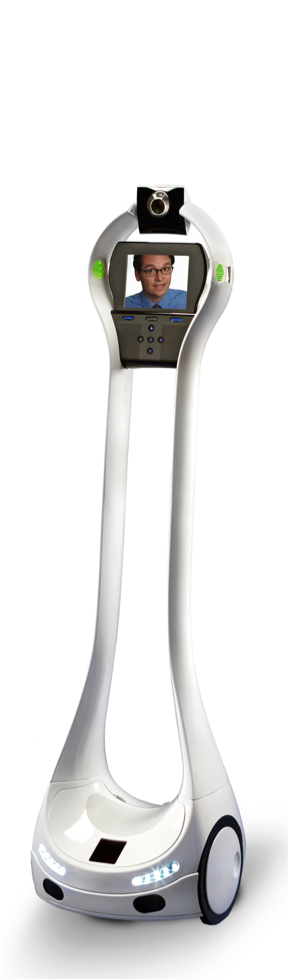
\includegraphics[width=0.66\textwidth]{bilder/grundlagen/1.png} 
      \subcaption{VGo}\label{fig:w} 
   \end{minipage}% 
   \hfill
   \begin{minipage}[t]{.25\linewidth} 
      \centering 
      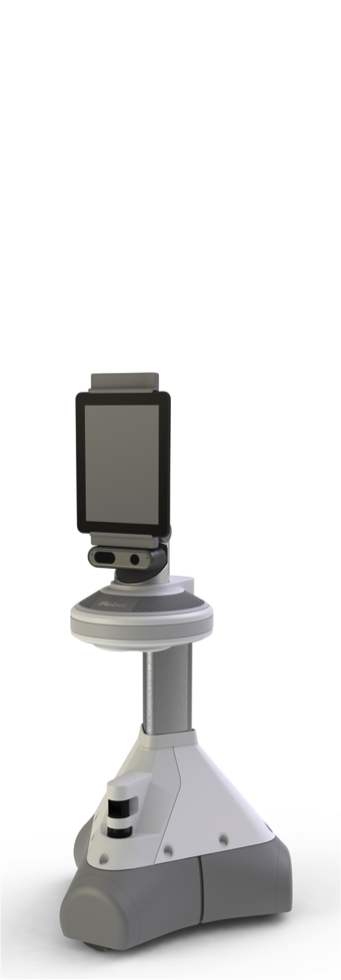
\includegraphics[width=0.78\textwidth]{bilder/grundlagen/2.png} 
      \subcaption{iRobot Ava}\label{fig:x} 
   \end{minipage}%
   \hfill
   \begin{minipage}[t]{.25\linewidth} 
      \centering 
      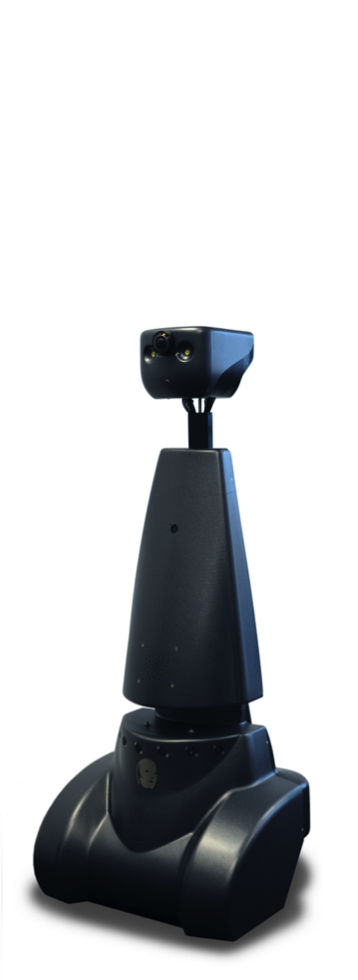
\includegraphics[width=0.8\textwidth]{bilder/grundlagen/3.png}
      \subcaption{Gostai Jazz}\label{fig:y} 
   \end{minipage}%
   \hfill
   \begin{minipage}[t]{.25\linewidth} 
      \centering 
      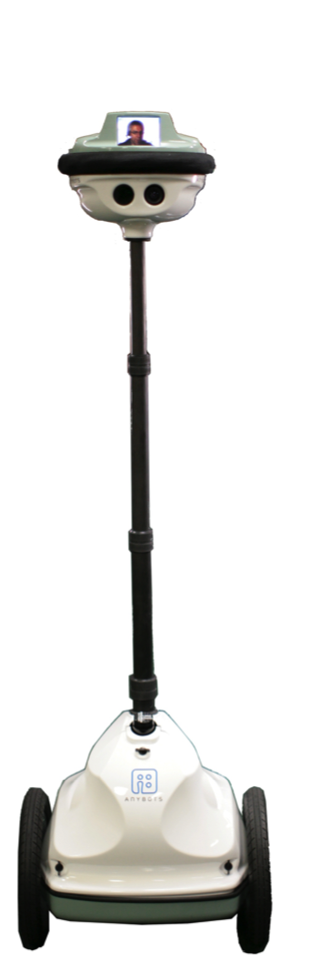
\includegraphics[width=0.7\textwidth]{bilder/grundlagen/4.png} 
      \subcaption{Anybots QB}\label{fig:z} 
   \end{minipage}%
   \hfill
   \caption{Eine Auswahl an \aclp{tps} im Vergleich. Zu Erkennen sind die Komponenten der einzelnen Telepräsenzrobotersysteme wie beispielsweise die Videokomponente, die eine Abbildung der benutzenden Person darstellt, und eine oder mehrere Videokameras, die die Umgebung filmen. Zu erkennen ist auch der unterschiedliche Aufbau der Systeme. (Bilder: aus  \cite{Kristoffersson2013})}\label{fig:bilder} 
\end{figure} 

Der Nutzen der Systeme zeigt sich in unterschiedlichen Anwendungsgebieten. Der folgende Abschnitt orientiert sich vornehmlich an den Ausführungen von \cite{Kristoffersson2013} und beschreibt allgemeine Anwendungsfelder von \acs{tps}.

\subsection{Anwendungsgebiete von Telepräsenzrobotersystemen}
\label{section:anwendungTPS} 

Die im Abschnitt \ref{subsection:komponenten} beschriebenen Eigenschaften und Komponenten der \aclp{tps} können innerhalb einiger Anwendungsfelder sinnvoll angewandt werden. So beschreibt \cite{Kristoffersson2013} Anwendungsgebiete im Bereich der Medizin, Gesundheitsversorgung, aber auch im Umfeld von Bürotätigkeiten und sicherheitsrelevanten Bereichen. Die folgende Aufzählung zeigt einen Überblick über die erwähnten Anwendungsfelder: %Anwendungsszenarien in der Medizin und Gesundheitsbereich werden  Im speziellen wird es um das Anwendungsfeld der Gesundheitsversorgung von Patienten mit Sprach- und Bewegungseinschränkung gehen, da dies im Fokus der Abschlussarbeit steht.

\begin{description}
\item[Unternehmens- und Büroaktivitäten] In global agierenden Unternehmen wird beispielsweise aufgrund der Vernetzung der Mitarbeiter in \ua international kooperierenden Gruppen ein immer größerer Wert auf die Kommunikation gelegt. \acs{tps} können in diesem Umfeld die Kommunikation und Kooperation untereinander sinnvoll ergänzen. Bereits 2002 gab es erfolgreiche Versuche, die Anwendung von mobilen \acs{tps} beispielsweise in  Unternehmenskonferenzen oder Sitzungen zu testen \cite{Jouppi}. Der Wunsch, \acs{tps} in wirtschaftlichen Szenarien zu etablieren, kann einmal in der Zeitersparnis durch das Wegfallen eventueller Reiseaktivitäten als auch in einer unmittelbaren Bereitstellung von Wissen durch geeignete Mitarbeiter in jedem Augenblick gesehen werden \cite{Jouppi}. Auch für Führungskräfte kann die Einflussnahme unter Umständen durch \aclp{tps} erweitert werden.
\item[Sicherheitsrelevante Bereiche] Neben den Anwendungsgebieten in Unternehmen, kann man sich mobile \acs{tps} auch in Bereichen vorstellen, die Sicherheitsrisiken für einen Menschen darstellen. So wurden während der Nuklearkatastrophe in Fukushima 2011 das \acl{tps} \textit{PackBot} der Firma iRobot verwendet, um Erkundungen innerhalb erhöhter Strahlenexpositionsgebiete vorzunehmen\footnote{\url{https://de.wikipedia.org/wiki/Nuklearkatastrophe_von_Fukushima} (letzter Aufruf: 04. März 2017)}.
\item[Gesundheitsversorgung, Medizin] Auf diesem Gebiet gibt es mehrere interessante Anwendungsbeispiele. Stepan Sopin, ein an Leukämie erkrankter Schüler, konnte mit einem \acs{tps} namens \textit{R.BOT 100} während seines Genesungsprozesses am Unterricht teilnehmen\footnote{\url{http://www.newsamen.com/101339/robot-goes-to-school-for-sick-kids-video} (letzter Aufruf: 04. März 2017)}. Auch Fels et al. (2001) beschreibt Anwendungsfelder von \acs{tps} für Schüler und Studenten~\cite{Fels2001}. 


Für die Verwendung von mobilen Robotersystemen im Anwendungsgebiet der Gesundheitsversorgung, beispielsweise bei älteren Personen mit körperlichen Beeinträchtigungen, werden nach Tsui et al. (2011) prinzipiell folgende Szenarien als mögliche Anwendungsfälle unterschieden \cite{tsui2011}. Diese Szenarien können auch auf die für diese Arbeit im Fokus stehende Personengruppe angewandt werden.

\begin{figure}[ht]
   \begin{minipage}[b]{\linewidth} 
      \centering 
      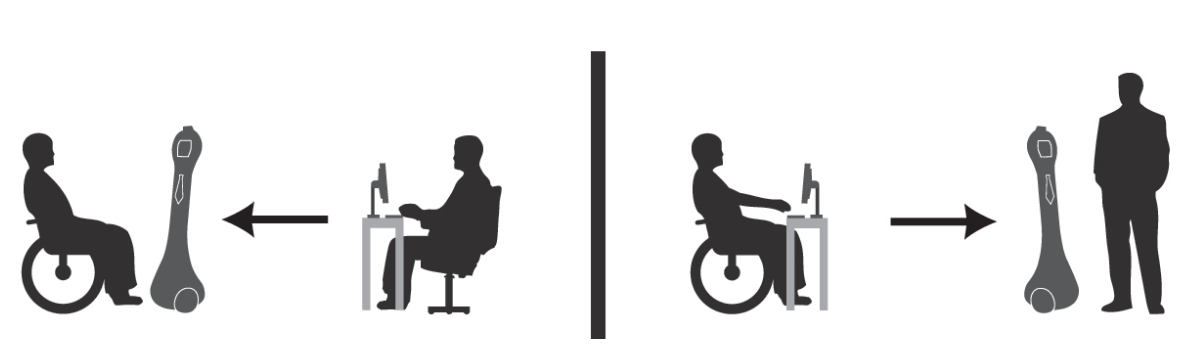
\includegraphics[width=0.7\textwidth]{bilder/grundlagen/Szenario.png}
      %\missingfigure{Darstellung aus Majaranta und Bulling (2014)}
   \end{minipage}% 
   \caption{(Links)~Szenario 1 \acs{tps} von Familienmitglied, Arzt oder Pflegekraft gesteuert, (Rechts)~Szenario 2 \acs{tps} von immobiler Person gesteuert (Bild: aus \cite[S.1]{tsui2011})}\label{fig:szenario} 
\end{figure} 

\begin{description}
\item[Szenarion 1] In diesem Szenario wird das \acs{tps} in die unmittelbare Umgebung der Person mit den körperlichen Beeinträchtigungen positioniert. Die Steuerung des \acs{tps} wird von Angehörigen, Ärzten oder Pflegepersonal übernommen. Dadurch ist es möglich, falls gewünscht, eine fast ununterbrochene Überwachung der hilfebedürftigen Person zu gewährleisten. Dieser Anwendungsfall wurde für Ärzte in Krankenhäusern bereits während der Visiten bei Patienten mit chirurgischen Eingriffen getestet \cite{Ellison2004}. Auch für Familienangehörige kann es sinnvoll sein, auf diese Art und Weise mit dem Familienmitglied zu interagieren.
\item[Szenarion 2] Das zweite Szenario steht im Fokus der vorliegenden Arbeit. Hierbei wird das \acs{tps} von einer Person mit Bewegungseinschränkung verwendet. Es wird in einer Umgebung positioniert, die seitens der Person mit der Bewegungseinschränkung erkundet oder mit der interagiert werden soll. Diese Umgebung kann auch die eigene Wohnung sein, wodurch der eingeschränkte Bewegungsumfang deutlich erweitert werden kann. Kinder, die beispielsweise krankheitsbedingt oder entfernungsbedingt nicht in der Schule anwesend sein können, können trotzdem durch die Unterstützung eines \acs{tps} wieder virtuell an der Klassengemeinschaft teilhaben\footnote{\url{http://www.dallasobserver.com/news/lyndon-baty-and-the-robot-that-saved-him-6429680} (letzter Aufruf: 08. Februar 2017)}. 
\end{description}
Für den Fall, dass das \acs{tps} in der Nähe der hilfebedürftigen Person verbleibt, sind die in Szenario 1 und 2 genannten Möglichkeiten kombinierbar. Ferner kann man sich eine Möglichkeit vorstellen, unterschiedliche Telepräsenzsysteme von einer Person zu kontrollieren, ähnlich wie es von Dr. Roey Tzezana, einem israelischen Wissenschaftler, vorgeschlagen wurde\footnote{\url{https://www.youtube.com/watch?v=zevLw5SbGvM} (letzter Aufruf: 08. Februar 2017)}.

\end{description}

Um \aclp{tps} im Rahmen der \og Anwendungsfelder adäquat nutzen zu können, muss eine gut funktionierende Teleoperation der Systeme gewährleistet sein. Daher geht der folgende Abschnitt auf die Teleoperation von Robotersystemen ein.

\subsection{Teleoperation von Robotersystemen}
\label{section:steuerung}

Eine gut funktionierende Steuerung eines mobilen Robotersystems ist für eine sichere und natürliche Interaktion in und mit der Umgebung (einschließlich der Personen in der Umgebung) eine wichtige Voraussetzung für die Akzeptanz des Systems \cite{Tsui2014}. Die Steuerung muss verlässlich und präzise die Steuerabsichten des Benutzers umsetzen. Hierbei sind neben dem Faktor der Umgebung (\zB~Hindernisse, Menschen und Tiere) auch die Vorerfahrungen der Benutzer im Umgang mit der Teleoperation von mobilen Robotersystemen relevant, wie die Arbeit von Casper und Murphy (2003) im Kontext der Terroranschläge in New York 2011 zeigt \cite{Casper2003,Labonte2010}.
Die visuellen Informationen und die implementierten Steuermethoden, die durch die Benutzerschnittstelle bereitgestellt werden, sind weitere Faktoren, die zu einer besseren situation~awareness und damit zu einer effizienteren Teleoperation von mobilen Robotersystemen beitragen \cite{Scholtz04,Yanco2004-2,Labonte2010,Tsui2014,Goodrich2013}.

%Gängige Systeme sind die haptischen und Grundsätzlich lassen sich hierbei 
Die Interaktion mit Robotersystemen erfolgt heutzutage weitgehend durch haptische Interaktionsmechanismen \cite{Dunser2015}, beispielsweise durch die Computermaus, die Tastatur oder einen Steuerhebel (Joystick). 

%Nach Peters et al. (2013) lassen sich haptische Eingabemechanismen nach aus der Physik bekannten mechanischen Gleichgewichtslagen einteilen, vgl. \cite[S.118]{Peters2013}. Hiernach wird zwischen \textit{stabilen}, \textit{labilen} und \textit{indifferenten} Gleichgewichtslagen unterschieden \cite{Peters2013}. Angewandt auf haptischen Eingabegeräte können sich in der Interaktion zwischen Eingabemechanismus und Benutzer die dynamischen Veränderungen des Mechanismus ebenfalls stabil, labil und indifferent Verhalten. Beispiel für



\begin{comment}
\begin{figure}[ht]
   \begin{minipage}[b]{\linewidth} 
      \centering 
\fbox{\includegraphics[width=\textwidth]{bilder/grundlagen/Kugel.png}}
   \end{minipage}% 
   \hfill
   \caption{}\label{fig:kugel} 
\end{figure}

\end{comment}


%Um eine Steuerung eines Computersystems zu ermöglichen von Heutzutage liegt der Schwerpunkt in Bezug auf die Interaktion mit einem Computersystemen 
 % einen Ein in der Mensch-Computer Interaktion besteht und und  sowohl für die Die Mensch-Computer Interaktion im Kontext der Teleoperation von Robotersystemen, stellt sowohl Anforderungen an das System als auch an den Benutzer selbst.

%Die Teleoperation von Robotersystemen basiert auf speziell entwickelte Benutzerschnittstellen, diese müssen um eine zielgerechte Interaktion über eine Distanz zu ermöglichen den Zustand des Telepräsenzsystems möglichst genau wiedergeben.

%Die Steuerung von Robotersystemen und damit der Informationstransfer von Mensch zu Computer basiert auf unterschiedlichen Eingabesystemen. 
Dabei lassen sich in Abhängigkeit des Einflusses des Benutzers auf die aktive Steuerung unterschiedliche Steuermethoden unterscheiden. Goodrich et al. (2013) unterscheidet folgende \cite{Goodrich2013}.
%Neben einer direkten Steuerung durch den Benutzer des \acs{tps} der dazu führt, dass alle an den mobilen Roboter übertragenen Signale vom Roboter umgesetzt werden lassen sich noch weitere erweiterte Steuermethoden nach G \cite{Goodrich2013}.
\begin{description}
\item[Supervisory control] Hierunter wird eine intermittierende Steuerungsmethode verstanden, wobei eine oder mehrere Benutzer nach jedem Steuerbefehl auf die Rückmeldung des Roboters warten; so kann Schritt für Schritt ein beabsichtigter Weg beschritten werden~\cite{sheridan1992}.
\item[Direct control] Darunter wird die direkte Umsetzung der Steuersignale durch das mobile Robotersystem verstanden. Die von Minsky visionierte Interaktion kann zu dieser Methode gezählt werden, \vgl~Abschnitt~\ref{section:tele}. 
\item[Shared control] Die steuernde Person sendet die beabsichtigten Steuerkommandos an den mobilen Roboter. Im Gegensatz zur direkten Kontrolle während der \textit{direct control}-Methode führt der mobile Roboter weiterhin die Steueranweisungen aus, verändert sie jedoch in Abhängigkeit von  auftauchenden sicherheitsrelevanten oder steuerungsrelaventen Aspekten, \zB beim Ausweichen eines Hindernisses. Dadurch kann sich der Benutzer auf andere Aspekte konzentrieren. Vergleiche dieser Methoden werden in \cite{Baldo2015} gezeigt.
\item[Traded control] Diese Methode erweitert die \textit{shared control}-Methode,- dahingehend, dass der Benutzer das Bewegungsziel vorgibt,- und der Roboter die Aufgaben eigenständig ausführt, bis die Aufgabe oder das Ziel erfüllt wurde.
\end{description}

Nach Abschluss der Beschreibung aller wichtigen Komponenten für die Umsetzung einer blick- und augenbasierten Steuerung eines mobilen Robotersystem mithilfe eines Eyetracking-Systems, wird in dem folgenden Kapitel~\ref{chapter:fragestellung} auf die vorgesehen Lösungsstrategien und die zu untersuchenden Testmerkmale eingegangen. 

%Die Steuerung einer Benutzeroberfläche mittels Blick- oder Augenbewegungen zu gewährleisten, stellt eine Herausforderung dar \cite{Hollomon2017}. Zwar ist die Augenmotorik willkürlich kontrollierbar, dennoch gibt es wie \og viele unwillkürliche Augenbewegung im Rahmen der Wahrnehmung und Orientierung. Es gilt somit, zwischen beabsichtigten Steuersignalen und unbeabsichtigten Blickbewegungen des Benutzers zu unterscheiden. Das Auge, welches primär als Sinnesorgan zur Perzeption der Umwelt dient, übernimmt wie in Abschnitt \ref{subsection:okumot} gezeigt, willkürliche Steueraufgaben durch die extraokuläre Muskulatur. Damit fungieren die Augenmuskulatur als Steuerinstanz, ähnlich wie es die Hand und Fingermuskulatur bei der Eingabe durch die Maus oder Tastatur erfüllen. Die Eingabemöglichkeit hängt mit den möglichen Augenbewegungen zusammen. In der vorliegenden Arbeit werden (Blickbewegungen, Lidschluss, Fixation, vertikaler Augenbewegung) als definierte Augengeste verwendet.



%\item Midas-Touch: Aufgrund der bereits \og Doppelfunktion des Auges als Sinnesorgan im Rahmen der visuellen Wahrnehmung und gleichzeitig als motorisches Effektororgan \zB Im Rahmen von Steueraufgaben kann es zum sogenannten Midas-Touch Problem kommen \cite{Majaranta2014}. Hierunter versteht man die Fehlinterpretation einer Augengeste als Steuersignal, wenn der Benutzer nur umher blickt und keine Steuerintention verfolgt. Im Unterschied zu einer Computermaus kann beispielsweise der \acs{por} als Mauszeiger nicht einfach an einer Stelle des Bildschirms belassen werden, während andere Bereiche des Bildschirms betrachtet werden. Dies ist bei der manuellen Steuerung mit der Computermaus ohne Probleme möglich. Auch das gewohnte \enquote{klicken} bei der Verwendung der Computermaus um \zB Buttons zu selektieren, kann nicht ohne Probleme in der Augensteuerung umgesetzt werden. Die Fixationen als Selektionsmechanismus können zu unabsichtlichen Betätigungen führen. Dies lässt sich zu einem gewissen Grade mittels der Kombination mehrerer Augengesten als Selektionsmechanismus beheben \cite{Majaranta2014}. 


%Grundsätzlich lassen nach Majaranta et al. sich Eyetracking-Systeme

%Majaranta und Bulling (2014) teilen die allgemeinen Nutzungsmöglichkeiten in vier Kategorien ein, siehe Abbildung \ref{fig:continuum}.

\begin{comment}


\begin{figure}[ht]
   \begin{minipage}[b]{\linewidth} 
      \centering 
      \includegraphics[width=1\textwidth]{bilder/grundlagen/D170203.png}
      %\missingfigure{Darstellung aus Majaranta und Bulling (2014)}
   \end{minipage}% 
   \caption{Mögliche Nutzungsmöglichkeiten von Eyetrackingdevices (Bild: \cite[S.52]{Bondke2014}) }\label{fig:continuum} 
\end{figure} 
\end{comment}
%So gibt es blickbasierte- Text Eingabesysteme für Menschen mit Bewegungseinschränkung. Diese Systeme ermöglichen es mittels eines zusätzlichen Kommunikationskanals, die Lebensqualität der Benutzer deutlich zu verbessern und ihr Leben ein Stück aktiver zu gestalten.


%\item Genauigkeit: Der entscheidente Faktor für die Genauigkeit der Eyetrackingmethode sind die 

%\end{itemize}
%In der Literatur werden 5 explizite Blickgesten für die Steuerung untersucht. 
%(a) Fixation mit unterschiedlichen Intervallen, (b) Blinzeln und Zwinkern, (c) 



\begin{comment}

Es ergibt sich hierdurch die Möglichkeit der individuellen Nutzung des Eyetrackings für eine große Bandbreite von Anwendungsgebiete unter anderem für wissenschaftliche Zwecke \cite{SMI2011}.

Im Rahmen dieser Abschlussarbeit werden die  All diese Messparameter sich für unterschiedliche Anwendungsfelder relevant. Für einen Überblick sei auf die Ausführungen von Duchowski (2002) verwiesen \cite{Duchowski2002}.


Es folgt eine   Die Bewegung der Augenbulbi wird auf unterschiedliche Messmethoden . und die Augenbewegungen aufzuzeichnen und hieraus mittels verschiedener Messverfahren den \acf{por} des Benutzers zu berechnen. D Die Bestimmung des \acs{por} durch Eyetracking-Systeme benutzen unterschiedliche unterschiedliche anatomisch-physiologischen Eigenschaften des Auges die Augenbewegungen.   



Die Bestimmung der Blickposition wird durch ein Messverfahren ermöglicht welches auf der Distanz zwischen dem Mittelpunkt der Pupille und dem \og ersten Purkinjebild, welches durch die Reflektion einer Lichtquelle an der Vorderseite der Hornhaut entsteht. Dieser Messvorgang läuft völlig kontaktlos ab und benötigt lediglich eine adäuate Positionierung der Benutzenden Person vor der Lichtquelle.  Durch diese Möglichkeiten kommt das Eye-Tracking als technisches Hilfsmittel in vielen Anwendungsgebiete zu Einsatz. 

\subsection{Augenbasierte Interaktion}
Manuelle Eingabegeräte wie beispielsweise die Computermaus
Augenbewegungen als Steuersignale für ein Eingabegerät zu verwenden bietet sicherlich Nachteile 

%Für Marvin Minsky (09.08.1927 - 24.01.2016) lag in der Entwicklung von Telepräsenzrobotersystemen eine beträchtliche Innovationsmöglichkeit, von welcher er bereits in den achtziger Jahren überzeugt war \cite{Minsky1980}. So stellte er sich beispielsweise vor, Menschen mit Sensoren ausgestattete Kleidung benutzen zu lassen um damit entfernte Robotersysteme zu steuern, welche die gemessenen Bewegungen der Kleidungssensoren, eins zu eins in motorische Bewegungen des Roboters umsetzen können. Minsky ging sogar soweit, dass auch das Gefühl beispielsweise eine entfernte Roboterhand zu benutzen nicht von der Benutzung der eigenen Hand zu unterscheiden war. Damit habe man das Gefühl sich in der entfernten Umgebung anwesend zu fühlen, obwohl man sich dort nicht aufhält. 

%Die Wahrnehmung oder das Gefühl sich in einer anderen Umgebung als der aktuellen, präsent oder anwesend zu fühlen, bezeichnet Kristoffersson et al. als \textit{Telepräsenz} \cite{Kristoffersson2013}. Ein mobiles \acf{tps} ermöglicht es einem Benutzer, der dieses System steuert und durch die Komponenten des \acs{tps} einen Einblick in die entfernte Umgebung erhält, sich derartig mit dieser Umgebung zu verbinden, dass er sich in der entfernten Umgebung frei und unbeeinträchtigt von ortsbedingten Gegebenheiten der eigenen Umgebung bewegen kann \cite{Kristoffersson2013}. So kann der Benutzer die Umgebung des mobilen Roboters mittels einer oder mehrerer angebrachter Kameras virtuell verfolgen und erkunden. Der Benutzer fühlt sich aufgrund dieser Möglichkeiten an dem Ort des Roboters präsent \cite{sheridan1992,Tsui2014}.

%Ein derartiges mobiles \acl{tps} soll es einem Benutzer ermöglichen durch die Komponenten des \acs{tps} einen Einblick in die entfernte Umgebung zu erhalten und sich derartig mit dieser Umgebung zu verbinden, dass man sich in der entfernten Umgebung möglichst frei und unbeeinträchtigt von ortsbedingten Gegebenheiten der eigenen Umgebung bewegen kann \cite{Kristoffersson2013, sheridan1992,Tsui2014}.

 %einem Teilgebiet der Robotik, welches sich mit dem Bedienen von Robotersystemen beschäftigt, wobei die Bedienung über eine Entfernung erfolgt und somit keine direkte Steuerung am Robotersystem erfolgt  \cite{Rossler2009}. In diesem Zusammenhang eng verbunden ist


%Die Entwicklung von Methoden zur Aufzeichnung von Augenbewegungen geht zurück auf das Jahr 1879 \cite{Lupu2013}. Emile Java, einen französischen Augenarzt führte Selbstversuche beim Lesen durch. Hierbei benutzte er einen einfachen Spiegel und erkannte, dass verschiedene Phasen während der Augenbewegung zu unterscheiden sind , wie die Sakkaden und Fixation \cite{Lupu2013}. Es folgten Entwicklungen zu invasiven Methoden mittels Kontaktlinsen von Edmund Huey (1908). Doge und Cline konnten 1901 bereits einen nicht inversive Methode eines Eyeträckers auf Basis des \og Cornealreflexes erstellen. Hierdurch war es möglich die Geschwindigkeit von Augenbewegungen genau zu bestimmen, jedoch nur für horizontale Augenbewegungen.



\textcolor{red}{
Die Augen erfüllen eine zentrale Funktion in der menschlichen Kommunikation. Der Blickkontakt ist oftmals ganz entscheidend für das gegenseitiges Vertrauen. Blickrichtung und Bewegung liefern Einblicke in innere Einstellungen und Absichten von Personen. So sind die Augen, wie man sagt, der Spiegel zur Seele eines Menschen. Für Menschen mit Bewegungseinschränkungen sind die Augen oftmals die einzige Kommunikationsmöglichkeit und aus diesem Grund umso entscheidender an der Kommunikation mit der Umgebung beteiligt. Es gibt vielfältige Möglichkeiten wie es zu einer Bewegungseinschränkung mit körperlichen Beeinträchtigungen kommen kann. So können Traumata, infektiöse Erkrankungen, Erbkrankheiten, Durchblutungsstörungen oder Autoimmunerkrankungen zu einer schwerwiegenden Beeinträchtigung führen. All diese Personengruppen können von unterstützenden technischen Systemen profitieren. Im folgenden wird ein Überblick über die verschiedenen Trackingmethoden und Systeme geliefert. \tp sind bereits seit mehreren Jahrzehnten in der Forschung als hilfreiches Werkzeug zur Erforschung kognitiver Prozesse und Intentionen der Benutzer in Anwendung. Sie haben Einblicke und Erkenntnisse geliefert, welche heute beispielsweise in Marketingbereichen Anwendung finden. Die Benutzung von Eyetrackingssystemen als Eingabemedium scheint eine weitere wichtige Möglichkeit der Nutzung zu sein. Speziell für Menschen mit körperlichen Einschränkungen bieten sich neue Möglichkeiten. So gibt es Blickbasierte- Text Eingabesysteme für Menschen mit Bewegungseinschränkung. Diese Systeme ermöglichen es mittels eines zusätzlichen Kommunikationskanal die Lebensqualität der Benutzer deutlich zu verbessern und ihr Leben ein Stück aktiver zu gestalten.
}


\end{comment}

%Wichtig \bzgl der Genauigkeit sind die Bildrate und die Auflösung der Videokamera.
%Bei Mobilen Systemen befindet sich die Kamera näher am Auge und liefert ein Bild mit mehr Pixels, welches sicher analysiert werden kann.

%Für die vorliegende Arbeit ist die Detektion von Augengesten im Rahmen einer Interaktion mit einer grafischen Benutzerschnittstelle relevant. Nachfolgend werden Augengesten als Eingabesignale für eine Benutzeroberfläche beschrieben. 
%Eine weitere, für die vorliegende Arbeit relevante Möglichkeit, liegt in der Nutzung der Augen- und Blickbewegung als Steuersignal \cite{Hollomon2017,Majaranta2014}. So kann der Benutzer den \acs{por} als Eingabe für die Bewegung des Mauszeigers nutzen und diesen entsprechend bewegen. Hierdurch können kleinen Symbolgrafiken (Icons) einer Benutzeroberfläche beispielsweise durch längere Fixation oder Zwinkern selektiert werden, ähnlich wie eine Bedienung mit der Computermaus. Diese Art der Interaktion kann so ausgelegt werden, dass keine zusätzliche manuelle oder andersartige Interaktion notwendig ist und so rein auf Grundlage der motorischen Fähigkeiten der Augen- und Lidmuskulatur basiert. Das folgende Kapitel stellt Eyetracking-Systeme als eine Steuerkomponente vor.
%These kinds of trackers usually consist of a standard desktop computer with an infrared camera mounted beneath (or next to) a display monitor, with image processing software to locate and identify the features of the eye used for tracking. In operation, infrared light from an LED embedded in the infrared camera is first directed into the eye to create strong reflections in target eye features to make them easier to track (infrared light is used to avoid dazzling the user with visible light). The light enters the retina and a large proportion of it is reflected back, making the pupil appear as a bright, well defined disc (known as the “bright pupil” effect). The corneal reflection (or first Purkinje image) is also generated by the infrared light, appearing as a small, but sharp, glint (see Figure 1).Figure


\begin{comment}


Die Systeme machen sich nach Young und Sheena (1975)  unter anderem folgende Charakteristika zur Detektion zunutze:

\begin{itemize}
\item Lichtreflexion von speziellen Kontaktlinsen.
\item  Videobilder der Pupille und der Iris.
\item elektrische Potentialdifferenz zwischen der Vorder- und Hinterseite des Augapfels.
\end{itemize}


Einige der Systeme machen sich zur Positionsbestimmung die \og anatomischen und physiologischen Eigenschaften der Augen zunutze \cite{Joos2003}. Mittels der Position der Augen lassen sich Parameter, wie der sogenannte \acf{por} des Benutzers berechnen. Der \acs{por} ist der aktuelle Betrachtungspunkt im Blickfeld eines Nutzers, der aus der Augenstellung berechnet werden kann. 
Die meisten Eyetraking-Systeme bestimmen den \acs{por} durch einen Algorithmus, der Sich die Refelxion der Cornea, also das Purkinje Bild (P1) in Relation des Pupillenzentrums zunutze macht. corneal-reflection/pupil-centre
%Most commercial eye-tracking systems available today measure point-of-regard by the “corneal-reflection/pupil-centre” method (Goldberg & Wichansky, 2003). 

\end{comment}
  
  % Kapitel 3
 % kapitel3.tex
\externaldocument{02_grundlagen}
\externaldocument{04_implementierung}
\chapter{Fragestellung und Testmerkmale}
\label{chapter:fragestellung}

\section{Modellbildung}
\label{section:modellbildung}
Der im Rahmen dieder Abschlussarbeit vorgestellte Softwareprototyp basiert auf Vorarbeiten von Eidam et al. (\vgl \cite{Eidam2015,Eidam2016}) und dem aus dieser Arbeit entwickelten Softwareprototyp. Als eine alternative Kommunikationsmöglichkeit für Personen mit Sprach- und Bewegungseinschränkungen ermöglicht der Prototyp von Eidam et al. die Identifikation und Sonifikation von Bildobjekten auf austauschbaren Bildern mithilfe eines Eyetrackers. Diese vorliegende Arbeit erweitert diesen Ansatz um die Implementierung zweier unterschiedlicher Steuerungsmodelle für ein mobiles Robotersystem und um die Darstellung dynamischer Inhalte im Sinne eines Videobildes als \enquote{Live-Ansicht} im Vergleich zu statischen Inhalten.

Das in \acs{abb} \ref{fig:infotrans} skizzierte technisch unterstützte Kommunikationsverhalten zwischen Mensch und Umgebung,- kann nach Einführung der beteiligten Komponenten aus Kapitel \ref{chapter:grundlagen} zum erweiterten geplanten Interaktionsmodell für den Softwareprototyp ausgebaut werden.

\begin{figure}[ht]
\begin{minipage}[t]{\linewidth} 
      \centering 
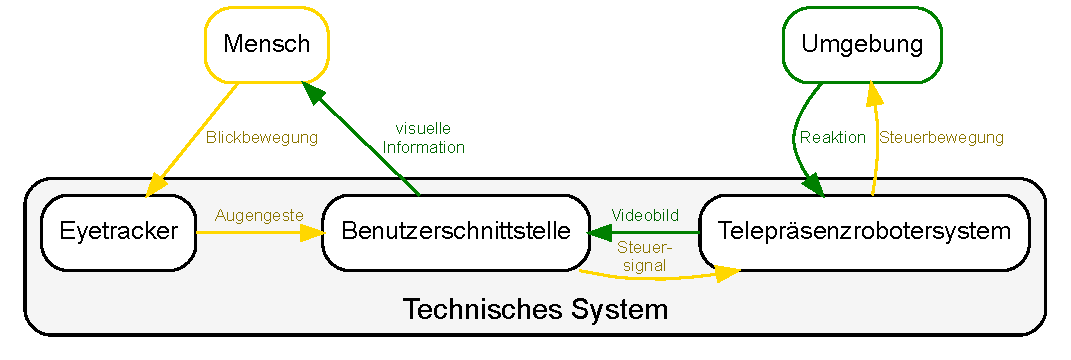
\includegraphics[width=\textwidth]{bilder/implementierung/komptrans.pdf}
   \end{minipage}% 
\caption{Die technisch unterstützte Kommunikation zwischen Mensch und Umgebung. Erweiterung der in \acs{abb}. \ref{fig:infotrans} auf Seite \pageref{fig:infotrans} grundsätzliche Ablauf der Kommunikation. Der Fokus liegt nun auf der Interaktion der einzelnen Komponenten des Systems.}
\label{fig:infotrans2}
\end{figure}

Die implementierten Steuerungsmodelle für das mobile Robotersystem sollen mittels eines selbst konzipierten Fragebogens untereinander verglichen und hinsichtlich der Machbarkeit, der Präzision, des Handlings, der Ermüdung und der Nutzung eines Panikschalters bewertet werden. 

Es folgt eine kurze einführende Beschreibung der beiden Steuerungsmodelle und Testmerkmale.

\section{Steuerungsmodell}
\label{section:steurungsmodell} 

\begin{comment}
\end{comment}
Nach Peters et al.~(2013) lassen sich haptische Eingabemechanismen nach mechanischen Gleichgewichtslagen aus der Physik einteilen, \vgl~\cite[S.118]{Peters2013}. Hiernach wird zwischen \textit{stabilen}, \textit{labilen} und \textit{indifferenten} Gleichgewichtslagen unterschieden, siehe \acs{abb}~\ref{fig:kugel} \cite{Peters2013}. Angewandt auf haptischen Eingabegeräte können sich in der Interaktion zwischen Eingabemechanismus und Benutzer die dynamischen Veränderungen des Mechanismus ebenfalls stabil, labil und indifferent verhalten.

\begin{figure}[ht]
\centering 
  \begin{minipage}[b]{0.8\linewidth} 

\includegraphics[width=\textwidth]{bilder/grundlagen/kugelang.pdf}
   \end{minipage}% 
   \hfill
   \caption{Mechanische Gleichgewichtslagen (\textit{stabil}, \textit{labil} und \textit{indifferent}) aus der Physik veranschaulicht am Beispiel einer Kugel \cite{Peters2013}. (Bild: angelehnt an \cite[S.118]{Peters2013})}\label{fig:kugel} 
\end{figure}

Allgemein können die bewährten Konzepte und Eigenschaften der haptischen Eingabegeräte auf grafische Steuerelemente übertragen werden. Auf dieser Grundlage wurde zur Steuerung eines mobilen Roboters, basierend auf Blickbewegungen, als erste Lösungsstrategie ein \textit{diskretes}~Steuermodell implementiert. Unter diesm Begriff des \textit{diskreten}~Steuermodells, wie er im Rahmen dieser vorliegenden Arbeit verwendet wird, ist eine Steuermethode zu verstehen, die nur während der Betätigung eines Steuerelements (siehe Kapitel~\ref{subsection:robotsteuerung}) ein vorgegebenes Bewegungssignal erzeugt. Damit handelt es sich, wie bei Peters et al.~(2013) beschrieben, um einen, in Analogie zu haptischen Eingabemechanismen, \textit{monostabilen} Mechanismus für den Informationstranfer \cite{Peters2013}. Das Steuerelement nimmt nur zwei endliche Wertzustände (\enquote{nicht betätigt = keine Bewegung}, \enquote{betätigt = festgelegte Bewegung}) an und wechselt jeweils in den Ausgangszustand (hier, in den Zustand \enquote{nicht betätigt}), falls keine Betätigung stattfindet. Die Betätigung des Steuerelements erfolgt durch eine Blickgeste (\acs{por} des Benutzers) innerhalb des angezeigten Bereiches eines Steuerelementes, (\vgl Kapitel~\ref{subsection:robotsteuerung}).

%Als erste Lösungsstrategie zur Steuerung eines mobilen Roboters, basierend auf Blickbewegungen, wurde ein \textit{diskretes} Steuermodell implementiert. Unter dem Begriff des \textit{diskreten} Steuermodells, wie es im Rahmen dieser vorliegenden Arbeit verwendet wird, ist eine Steuermethode zu verstehen, die nur während der Betätigung eines Steuerelements (siehe Kapitel \ref{subsection:robotsteuerung}) ein vorgegebenes Bewegungssignal erzeugt. Damit handelt es sich wie bei Peters et al. (2013) beschrieben um einen, in Analogie zu haptischen Eingabemechanismen, \textit{monostabilen} Mechanismus für den Informationstranfer \cite{Peters2013}. Das Steuerelement nimmt somit letztlich nur zwei endliche Wertzustände (\enquote{nicht betätigt = keine Bewegung}, \enquote{betätigt = festgelegte Bewegung}) an und wechselt jeweils in den Ausgangszustand. Die Betätigung des Steuerelements erfolgt durch eine Blickgeste, also den \acs{por} des Benutzers. 

Eine zweite Steuerungsform wurde als \textit{kontinuierliche} Steuermethode konzipiert. Diese Form des Informationsaustausches kann nach Peters et al.~(2013) in Analogie zu haptischen Eingabemechanismen als \textit{indifferenter} Mechanismus bezeichnet werden. Im Unterschied zu der \textit{diskreten} Steuermethode, erfolgt eine kontinuierliche Befehlserzeugung innerhalb eines definierten Wertebereichs (\enquote{keine Bewegung}-\enquote{maximale Bewegung}). Diese Werte werden durch jede Blickbewegung verändert. Diese Art der Steuerung ermöglicht eine differenzierte geschwindigkeits- und richtungsabhängige Befehlscodierung.  

\subsection{Diskretes Steuerungsmodell}
Das diskrete Steuerungsmodell stellt vier unterschiedliche Bewegungsrichtungen zur Verfügung. Hierbei werden zwei translationale Bewegungen in Vorwärts- und in Rückwärtsrichtung angeboten und jeweils die Drehung nach links und rechts. Somit ist diese Art der Steuerung vergleichbar mit einer Tastatursteuerung über die vier Richtungspfeiltasten\footnote{\url{https://de.wikipedia.org/wiki/Pfeiltaste} (letzter Aufruf: 18. Februar 2017)}. Die Bewegung findet jeweils während der Betätigung der Tasten statt. 

\subsection{Kontinuierliches Steuerungsmodell}
Wie eingangs erwähnt, stellt das kontinuierliche Steuermodell einen \textit{indifferenten} Eingabemechanismus bereit. Die Augen des Benutzers fungieren dabei als eine Art Steuerhebel (\enquote{Joystick})\footnote{\url{https://de.wikipedia.org/wiki/Joystick} (letzter Aufruf: 18. Februar 2017)}, wobei die beim Joystick gewohnte Rückkehr zur neutralen Ausgangsposition im vorliegenden Fall nicht passiv geschieht. Es ist leicht vorzustellen, dass jede Augenbewegung des Benutzers ein verändertes Bewegungssignal im Vergleich zum vorangegangen Befehl darstellt. Hierbei wurde zur Reduktion der Midas-Touch- Problematik eine Art \enquote{Neutralzone} im Zentrum des Blickfeldes durch einen farblich gekennzeichneten Bereich festgelegt, siehe Abschnitt~\ref{subsection:robotsteuerung}. Als Steuersignal werden die Blickbewegungen in Relation zur \enquote{Neutralstellung} im Sinne einer Translations- und Rotationsbewegung durch einen Algorithmus interpretiert. Translations- und Rotationsbewegungen können im Unterschied zur diskreten Steuerung in einer Bewegung simultan ausgeführt werden. Hierdurch soll ein erweiterter Bewegungsumfang im Vergleich zur diskreten Steuerungsmethode bereitgestellt werden.

\section{Testmerkmale der Steuerung}
\label{sect:testmerkmale}
Die beschriebenen Steuerungsmodelle werden anhand quantitativer und qualitativer Merkmale mithilfe des Fragebogens und der Parcoursbewältigungsaufgabe untersucht. Es folgt eine Auflistung der untersuchten Items. 
\begin{enumerate}
  \item Zur Klärung der Präzision und Machbarkeit der einzelnen Steuerungsmodelle wurde eine Parcoursaufgabe konzipiert und die Dauer, die zur Bewältigung benötigt wurde, quantifiziert.
  \item Die Frage der Präzision wurde mittels diochtomer Mehrfachantworten \bzgl unerwünschter Ausführungen während des gesamten Durchführungszeitraums erweitert. Hierfür wurden unerwünschte Ausführungen für folgende Merkmale erfragt: 
  \begin{enumerate}
  \item Blickbewegung
  \item Lidschluss
  \item Horizontale Augengeste
  \item Vertikale Augengeste
  \item Stoppmechanismus
  \item Steuerungskomandos
  \item Moduswechsel
  \item Sonstige
  \end{enumerate}
  Das Merkmal \enquote{Sonstige} ermöglicht die Angabe weiterer unerwünschter Ausführungen. 
  \item Die Frage der Ermüdung wurde mittels einer vierstufigen Ratingskala bewertet, dabei bedeuten: \enquote{1 = nicht ermüdend}, \enquote{2 = wenig ermüdend}, \enquote{3 = ermüdend}, \enquote{4 = sehr ermüdend}. 
  \item Die Frage der Einfachheit des Handlings wurde mittels einer Ordinalskala mit den Merkmalsausprägungen (\enquote{1 = sehr einfach}, \enquote{2 = einfach}, \enquote{3 = schwer}, \enquote{4 = sehr schwer}) erhoben.
 \item Die Frage der Nutzung des Panikschalters wurde mittels einer Ordinalskala mit den Merkmalsausprägungen (\enquote{1 = sehr einfach}, \enquote{2 = einfach}, \enquote{3 = schwer}, \enquote{4 = sehr schwer}) erhoben.
  \item Jedes Steuerungsmodell wurde einzeln mittels einer Ordinalskala mit Schulnoten als Merkmalsausprägungen (\enquote{1 = sehr gut}, \enquote{2 = gut}, \enquote{3 = befriedigend}, \enquote{4 = ausreichend}, \enquote{5 = mangelhaft}, \enquote{6 = ungenügend}) erhoben.
\end{enumerate}
  
  % Kapitel 4
 % kapitel4.tex
\externaldocument{02_grundlagen.tex}
\externaldocument{03_fragestellung}
\chapter{Implementierung}
\label{chapter:implementierung}
Der folgende Abschnitt stellt die in Abschnitt~\ref{section:steurungsmodell} beschriebenen Modelle und ihre Implementierung im entwickelten Softwareprototyp dar. Zunächst wird auf die optischen Eigenschaften des Softwareprototyps eingegangen. Im Anschluss erfolgt eine Beschreibung der beiden technischen Komponenten des Systems sowie ihre Implementierung. Hierzu zählen das \et \iV der Firma \acf{smi} und das verwendete mobile Robotersystem (Roomba 620) der Firma iRobot® Corporation.

\section{Gestaltung der Benutzeroberfläche}
\label{sect:gui}
In Bezug auf die Erstellung einer grafischen Benutzeroberfläche (engl. \acf{gui}) wurde die grundlegende Struktur des Vorgängersystems von Eidam übernommen und um Elemente der Robotersteuerung und der Kameraverbindung erweitert, \vgl~\cite{Eidam2015}. Nachfolgend werden zusammenfassend die bestehenden Komponenten beschrieben. Der Fokus liegt auf den zur Vorgängerarbeit erweiterten Komponenten, explizit auf den Steuerungskomponenten.

\subsection{Allgemeine Komponenten der Benutzeroberfläche}
\acl{abb}~\ref{fig:diskretModeKomp} zeigt die vier wesentlichen Komponenten, die im Rahmen des Softwareprotyps verwendet wurden. Hierzu zählen die Menüleiste (1. rote Markierung), die Steuerelemente (2. gelbe Markierung, hier diskrete Steuerelemente), eine Statusleiste (3. blaue Markierung) und die aktuelle Darstellung der Kamerasicht (4. grüne Markierung). %Der \acs{por} des Benutzers erscheint als rot markierter Punkt im Zentrum der Darstellung und bewegt sich in Abhängigkeit der Blickbewegung.

\begin{figure}[ht]
\begin{center}
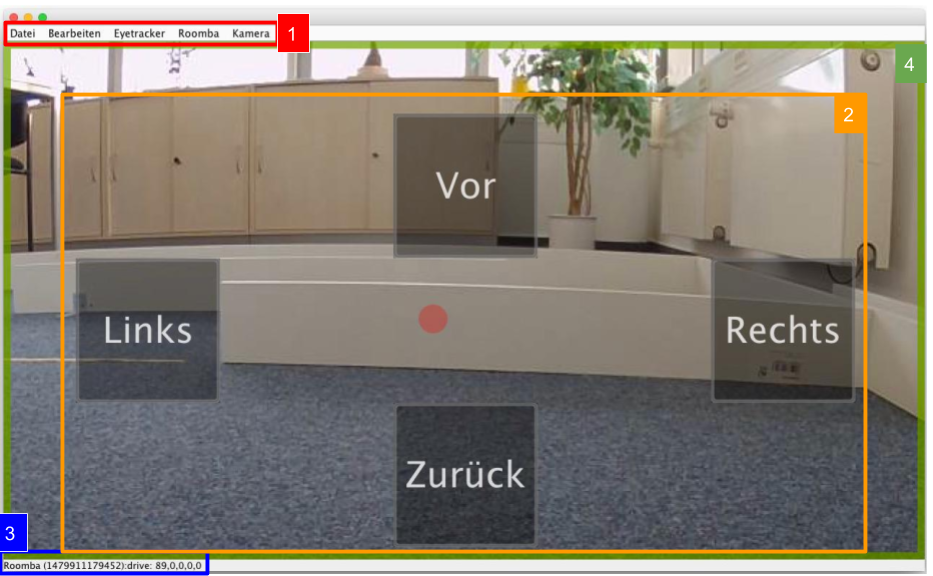
\includegraphics[width=0.7\textwidth]{bilder/implementierung/diskretMode1.png}
\end{center}
\caption{Darstellung der wesentlichen Komponenten des Softwareprototyps. (1)~Menüleiste mit den Punkten: Datei, Bearbeiten, Eyetracker, Roomba, Kamera. (2)~Steuerelemente (hier diskrete Steuerelemente). (3)~Statusleiste. (4)~Kamerapanel mit der Ansicht aus Sicht des mobilen Roboters. Der \acs{por} des Benutzers im Zentrum der Darstellung  erscheint als rot markierter Punkt.}
\label{fig:diskretModeKomp}
\end{figure}

Die Menüleiste (siehe \acs{abb}~\ref{fig:menu}) beinhaltet im Menüpunkt \enquote{Datei} neben der Möglichkeit, die Software zu starten und zu beenden, die Option, relevante Einstellungen in Bezug auf die Systemnutzung vorzunehmen. Der Menüpunkt \enquote{Eyetracker} ermöglicht,- neben dem Starten und Stoppen des Eyetrackings,- auch die vor jeder Nutzung notwendige Kalibrierung des Eyetrackers. Des Weiteren kann der \acs{por} an- \bzw ausgeschaltet werden. Auch die Möglichkeit, in einem Simulationsmodus den Eyetracker mit der Maus zu simulieren, ist gegeben. Ein Lidschluss kann dabei mit der rechten Maustaste simuliert werden \cite{Eidam2015}. Der Menüpunkt \enquote{Roomba} ermöglicht, die verbindungsrelevanten Einstellungen des mobilen Roboters (Roomba) anzupassen. Ferner wird die Möglichkeit des Resets und des Fahrens zur Ladestation gegeben. Der letzte Menüpunkt \enquote{Kamera} ermöglicht es, die kamerarelevanten Einstellungen vorzunehmen und anzupassen.
\begin{figure}[ht]
\begin{center}
   \begin{minipage}[t]{.4\linewidth} 
      \centering 
      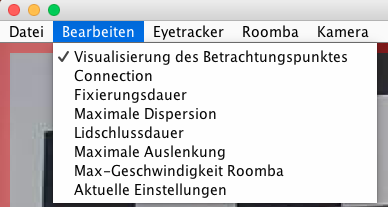
\includegraphics[width=1\textwidth]
      {bilder/implementierung/bearbeiten.png} 
      %\subcaption{Objekterkennunsmodus}
      \label{fig:l3} 
   \end{minipage}%
   %\hfill
    \begin{minipage}[t]{.4\linewidth} 
      \centering 
      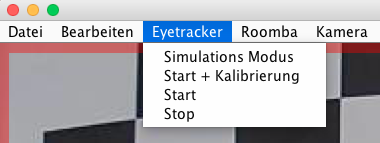
\includegraphics[width=1\textwidth]
      {bilder/implementierung/eyetracker.png} 
      %\subcaption{Objekterkennunsmodus}
      \label{fig:l3} 
   \end{minipage}%
   \hfill
   \begin{minipage}[t]{.4\linewidth} 
      \centering 
      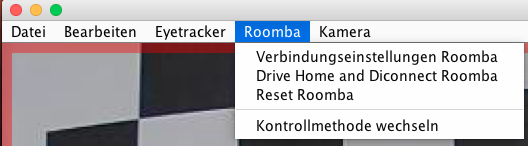
\includegraphics[width=1\textwidth]
      {bilder/implementierung/roomba.png} 
      %\subcaption{Steuerungsmodus}
      \label{fig:l2} 
   \end{minipage}%
   %\hfill
\begin{minipage}[t]{.4\linewidth} 
      \centering 
      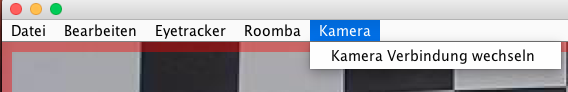
\includegraphics[width=1\textwidth]{bilder/implementierung/kamera.png} 
      %\subcaption{Betrachtungsmodus}
      \label{fig:l1} 
   \end{minipage}% 
   \hfill

\end{center}
\caption{Menüleiste mit den möglichen Menüauswahlpunkten.}
\label{fig:menu}
\end{figure}

Eine weitere, in \acs{abb}~\ref{fig:diskretModeKomp} nicht dargestellte Komponente, ist ein Pop-up-artiges Informationsfenster, das als ein visueller Feedbackmechanismus beispielsweise bei der erfolgreichen Kalibrierung des Eyetrackers oder bei der Verbindung mit dem mobilen Roboter für eine kurze definierte Zeitdauer erscheint. Dieser Mechanismus wurde von der Vorgängerversion übernommen, wobei in der aktuellen Version auf das akustische Feedback verzichtet wurde, siehe \acs{abb}~\ref{fig:info}, \vgl~\cite{Eidam2015}.

\begin{figure}[ht]
\begin{center}
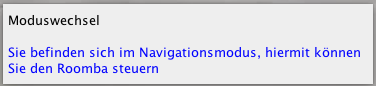
\includegraphics[width=0.6\textwidth]{bilder/implementierung/Infoframe.png}
\end{center}
\caption{Beispiel des Informationsframe als visueller Feedbackmechanismus. Mit \enquote{Navigantionsmodus} wird im vorliegenden Fall der \textsc{Steuerungsmodus} bezeichnet.}
\label{fig:info}
\end{figure}
\subsection{Gestaltung der Kontrollmodi}
\label{subsection:gestKontroll}
Die Benutzeroberfläche stellt drei unterschiedliche Modi zur Verfügung, durch die der Benutzer mit einer definierten Augengeste navigieren kann. Vorgesehen wurden die Modi:
\begin{enumerate}
\item \textsc{Betrachtungsmodus}
\item \textsc{Steuerungsmodus}
\item \textsc{Objekterkennungsmodus}
\end{enumerate}
Jeder dieser drei Modi stellt einen unterschiedlichen Funktionsumfang bereit, wobei der \textsc{Objekterkennungsmodus} nur demonstrativ für die geplante Objekterkennungsfunktion einer zukünftigen Softwarevariante steht, jedoch im aktuellen Prototyp keinerlei Funktionen bereithält. Die Modi werden durch eine unterschiedliche farbliche Außenranddarstellung gekennzeichnet (siehe~\acs{abb}~\ref{fig:modi}). Zunächst wird ein \textsc{Betrachtungsmodus} angeboten, der der Orientierung im Blickbereich dient und für die Interaktion mit der Menüleiste fungieren kann. Hierbei ist keine Steuerung des Telepräsenzrobotersytems möglich. Durch eine vertikale Blickbewegung erfolgt der Wechsel in den \textsc{Steuerungsmodus}. Hier findet die eigentliche Steuerung des \acs{tps} statt, wobei innerhalb des \textsc{Steuerungsmodus} mittels des Menüpunktes \enquote{Kontrollmethode wechseln} aus dem Menüleistenpunkt \enquote{Eyetracker} alternierend zwischen den beiden Steuermethoden (diskret und kontinuierlich) gewechselt werden kann, siehe~\acs{abb}~\ref{fig:menu}. 
Erfolgt eine weitere vertikale Blickgeste, so findet ein Wechsel in den \textsc{Objekterkennungsmodus} des Systems statt. Eine erneute vertikale Blickgeste führt zurück in den \textsc{Betrachtungsmodus}.
\begin{figure}[ht]
\begin{center}
\begin{minipage}[b]{.3\linewidth} 
      \centering 
      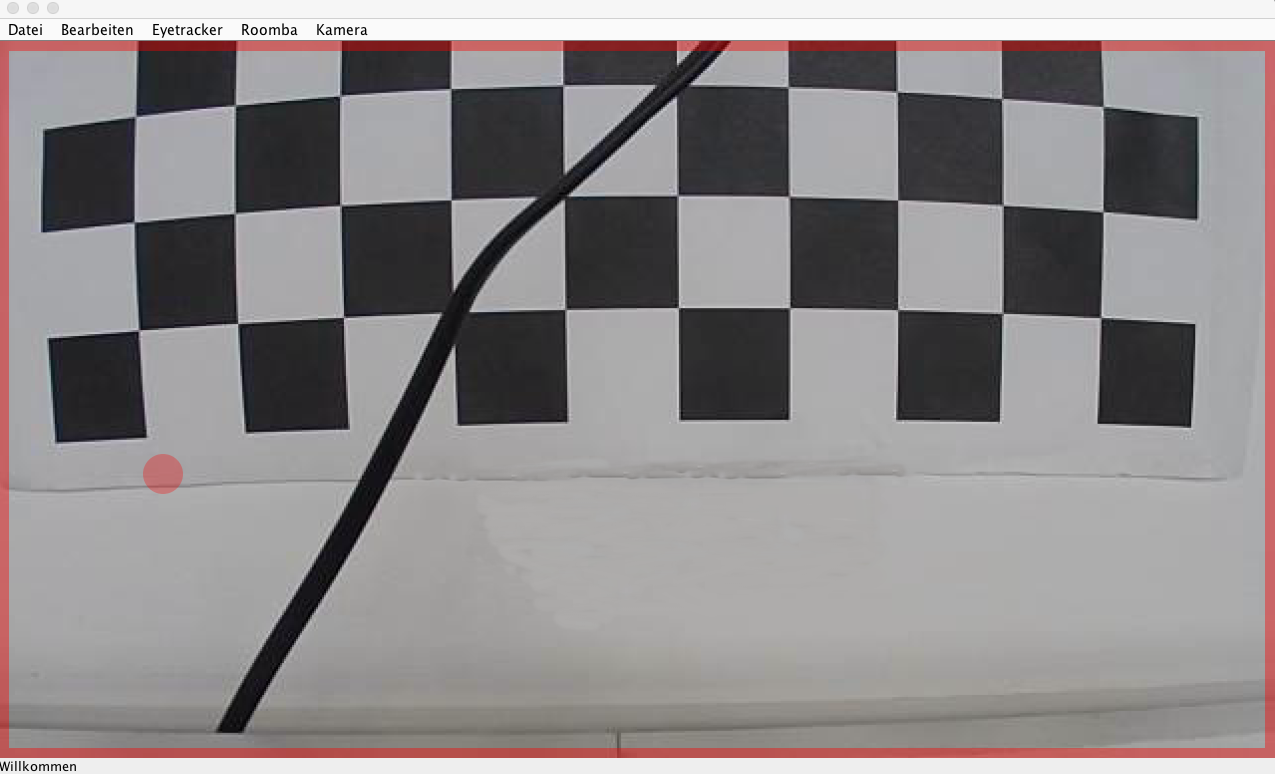
\includegraphics[width=1\textwidth]{bilder/implementierung/rot.png} 
      \subcaption{Betrachtungsmodus}
      \label{fig:l1} 
   \end{minipage}% 
   \hfill
   \begin{minipage}[b]{.3\linewidth} 
      \centering 
      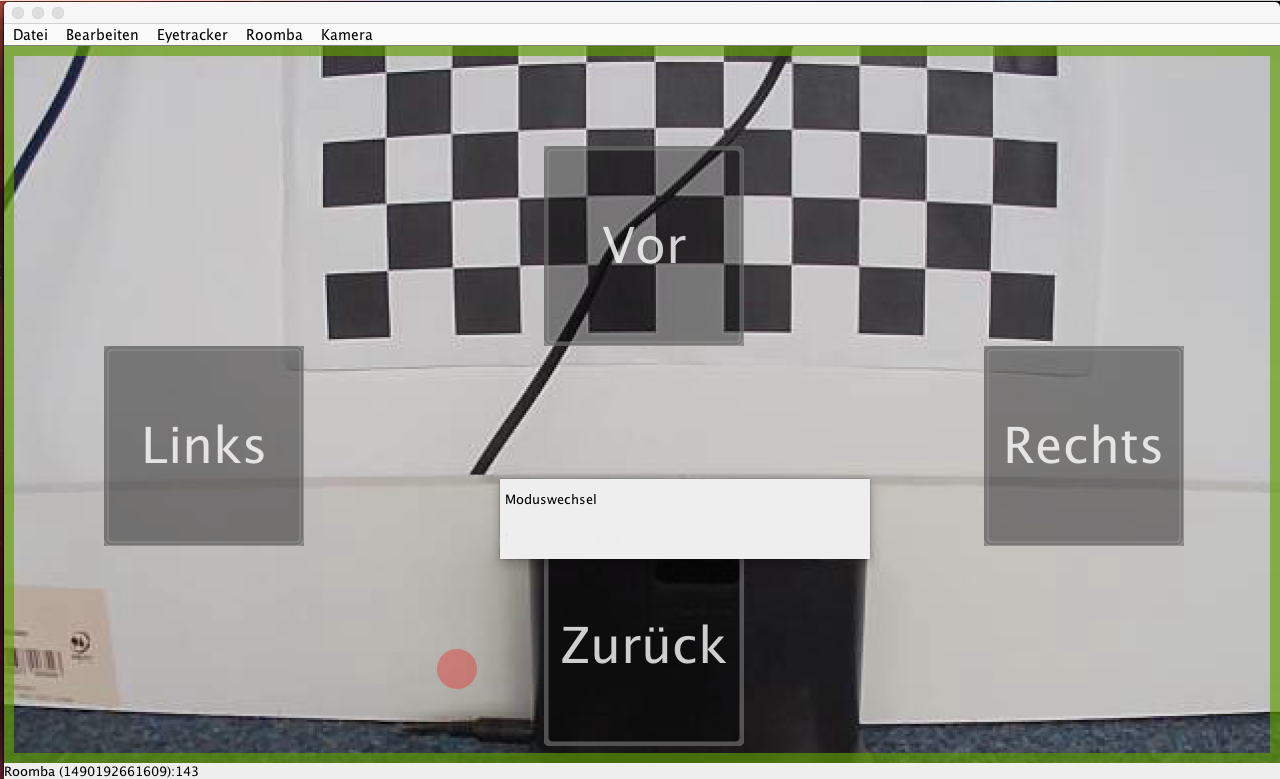
\includegraphics[width=1\textwidth]
      {bilder/implementierung/gruen.png} 
      \subcaption{Steuerungsmodus}
      \label{fig:l2} 
   \end{minipage}%
   \hfill
   \begin{minipage}[b]{.3\linewidth} 
      \centering 
      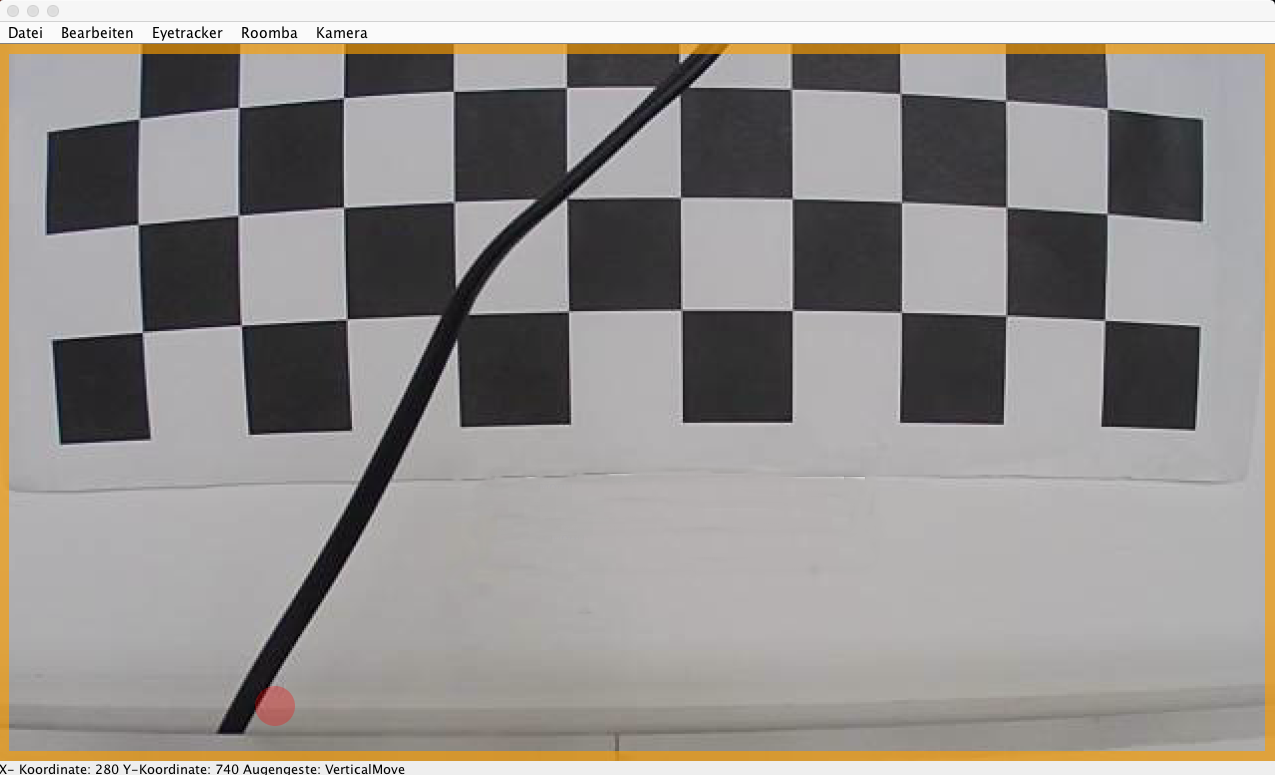
\includegraphics[width=1\textwidth]
      {bilder/implementierung/gelb.png} 
      \subcaption{Objekterkennungsmodus}
      \label{fig:l3} 
   \end{minipage}%
   \hfill
\end{center}
\caption{Darstellung der drei unterschiedlichen Kontrollmodi. Betrachtungsmodus~(rot), Steuerungsmodus~(grün), Objekterkennungsmodus (gelb).}
\label{fig:modi}
\end{figure}
Bei jedem Wechsel des Modus wird ein Informationsfenster als visueller Feedbackmechanismus angeboten. Dieser dient dazu, den aktuellen Modus zu benennen und dadurch eine einfachere Orientierung in der Programmführung zu ermöglichen.

\subsection{Gestaltung der diskreten Steuerung}
\label{subsection:gestDisk}
Zur Umsetzung der diskreten Steuerung wurden vier Steuerelemente (vor, zurück, links, rechts) auf dem Bildschirm angeordnet, siehe \acs{abb}~\ref{fig:diskretMode}. Diese wurden hierbei als teiltransparente Elemente konzipiert, um den Bereich \enquote{hinter} den Elementen nicht zu verdecken und möglichst den gesamten Blickbereich des \acs{tps} zur Orientierung und zur Bewegungsplanung zu nutzen. Der aktuelle \acs{por} des Benutzers wurde mittels eines teiltransparenten roten Punktes dargestellt und bewegt sich in Abhängigkeit der Blickbewegung, \vgl~\acs{abb}~\ref{fig:diskretMode}. Bei der Größenauswahl der Elemente wurde auf eine ausreichende Relation zwischen den elementfreien Bereichen der Blickfläche und der Größe der Elemente geachtet. Im Prototyp nehmen die Steuerelemente ca. 20 \% der Blickfläche ein und ermöglichen so einen größtenteils unbeeinträchtigten Blick auf die Bildfläche der Telepräsenskamera, gleichzeit sind die Flächen groß genug, um mittels der Augenbewegung selektiert zu werden. 
\begin{figure}[ht]
\begin{center}
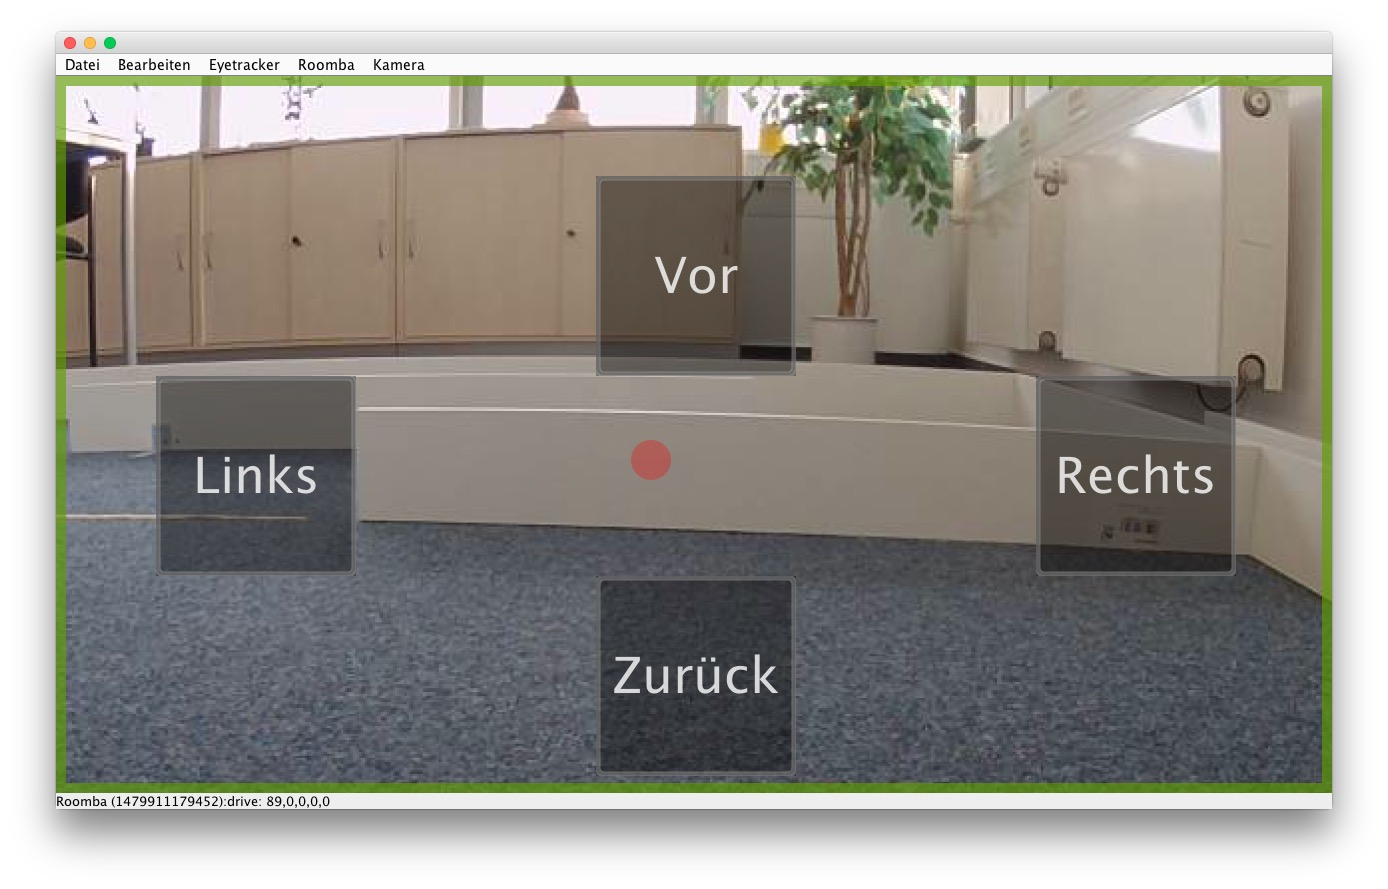
\includegraphics[width=\textwidth, height=100mm]{bilder/implementierung/diskretMode.JPG}
\end{center}
\caption{Darstellung der diskreten Steuerelemente (vor, zurück, links, rechts).}
\label{fig:diskretMode}
\end{figure}

\subsection{Gestaltung der kontinuierlichen Steuerung}
Zur Gestaltung der kontinuierlichen Steuerung wurde ein \enquote{Koordinatenkreuz} im Zentrum des Blickbereiches positioniert, siehe \acs{abb}~\ref{fig:contMode}. Ein farblich hervorgehobener Bereich in der Mitte des Blickfeldes wurde als \enquote{Neutralzone} konzipiert. Dadurch sollten das Midas-Touch-Problem reduziert und nur bewusste Steuerabsichten des Benutzers umgesetzt werden. Wurde der \acs{por} des Benutzers in diesen Bereich gerichtet, blieb das \acs{tps} unbewegt an seiner aktuellen Position stehen. Die Positionierung eines \enquote{Koordinatenkreuzes} sollte die Position der Neutralstellung veranschaulichen. Die Steuersignale wurden im Hinblick auf die Geschwindigkeits- und Richtungsamplitude anhand einer farblichen Abszissen- und Ordinatenachse in Abhängigkeit der Steuerbewegung abgebildet (in \acs{abb}~\ref{fig:contMode} durch den gelb und grünlich dargestellten Abschnitt im Bereich der \enquote{Neutralzone} nur schwer zu erkennen). Durch das Koordinatenkreuz ist es ferner möglich, eine Einteilung in vier verschiedenen Quadranten des Blickfeldes vorzunehmen (genauere Ausführungen im Abschnitt \ref{subsection:kontSt}).
\begin{figure}[ht]
\begin{center}
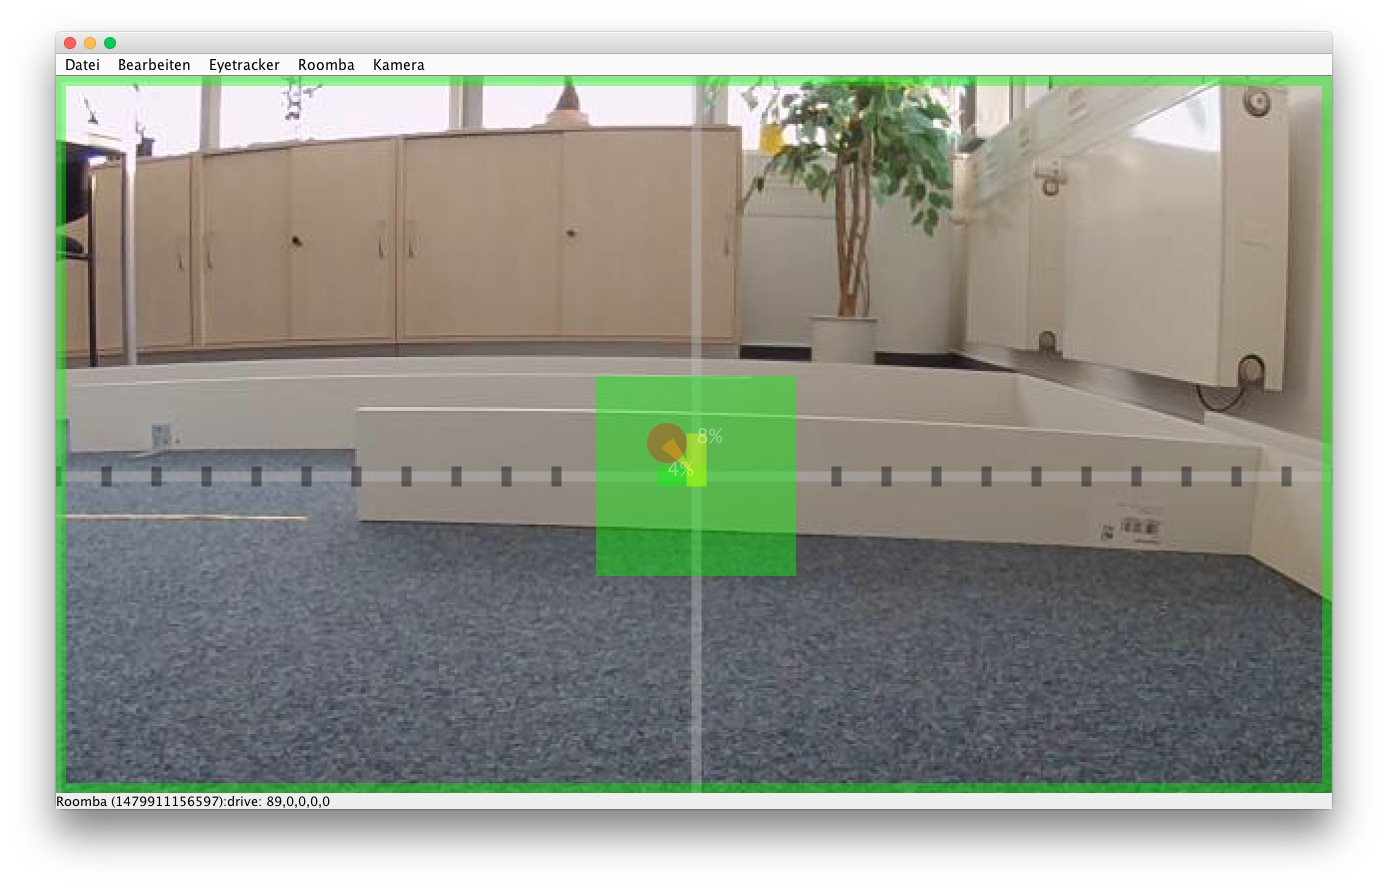
\includegraphics[width=\textwidth]{bilder/implementierung/continuousMode.JPG}
\end{center}
\caption{Darstellung der kontinuierlichen Steuerelemente. Zentral ist die \enquote{Neutralzone} farblich markiert. Dieser Bereich erzeugt keine Steuerbefehle und dient der Reduktion des Midas-Touch- Problems. Der rot markierte Punkt im Zentrum zeigt den \acs{por} des Benutzers.}
\label{fig:contMode}
\end{figure}


\section{Telepräsenzrobotersystem (TPS)}
\label{section:tpsI}
\subsection{iRobot Roomba 620}
Für die vorliegende Arbeit wurde als \tp ein \enquote{handelsüblicher} autonomer Staubsaugerroboter (Roomba 620) der Firma iRobot® Corporation benutzt, siehe \acs{abb}~\ref{fig:roomba}. Der Roomba ist seitens des Herstellers so konzipiert worden, dass dieser ohne technische Vorkenntnisse des Benutzers relativ einfach verwendet werden kann und hierbei weitgehend autonom funktioniert. Er eignet sich aufgrund einer seit 2005 vom Hersteller bereitgestellten offenen Schnittstellendokumentation (iRoomba Create Open Interface (OI))~\cite{IRobot2010} hervorragend zur Augmentation als \tp. Der Roomba ist somit durch die angebotene Befehlsstruktur der OI im Verhalten vielfältig zu kontrollieren. Um die für ein \tp benötigte visuelle Komponente zu gewährleisten, wurde der Roboter um eine zentrisch angeordnete Kamera erweitert, siehe \acs{abb}~\ref{fig:subroomba} auf Seite \pageref{fig:subroomba}. Zur Netzwerkkommunikation und entfernten Steuerung wurde ein Access-Point an der seriellen Schnittstelle des mobilen Roboters angebracht (\vgl~\acs{abb}~\ref{fig:subroomba}). Die vorinstallierten Bürsten des Staubsaugerroboters wurden aufgrund der Geräuschentwicklung und der fehlenden Funktion während des Gebrauchs entfernt. 

\begin{figure}[ht]
\begin{minipage}[b]{\linewidth} 
      \centering 
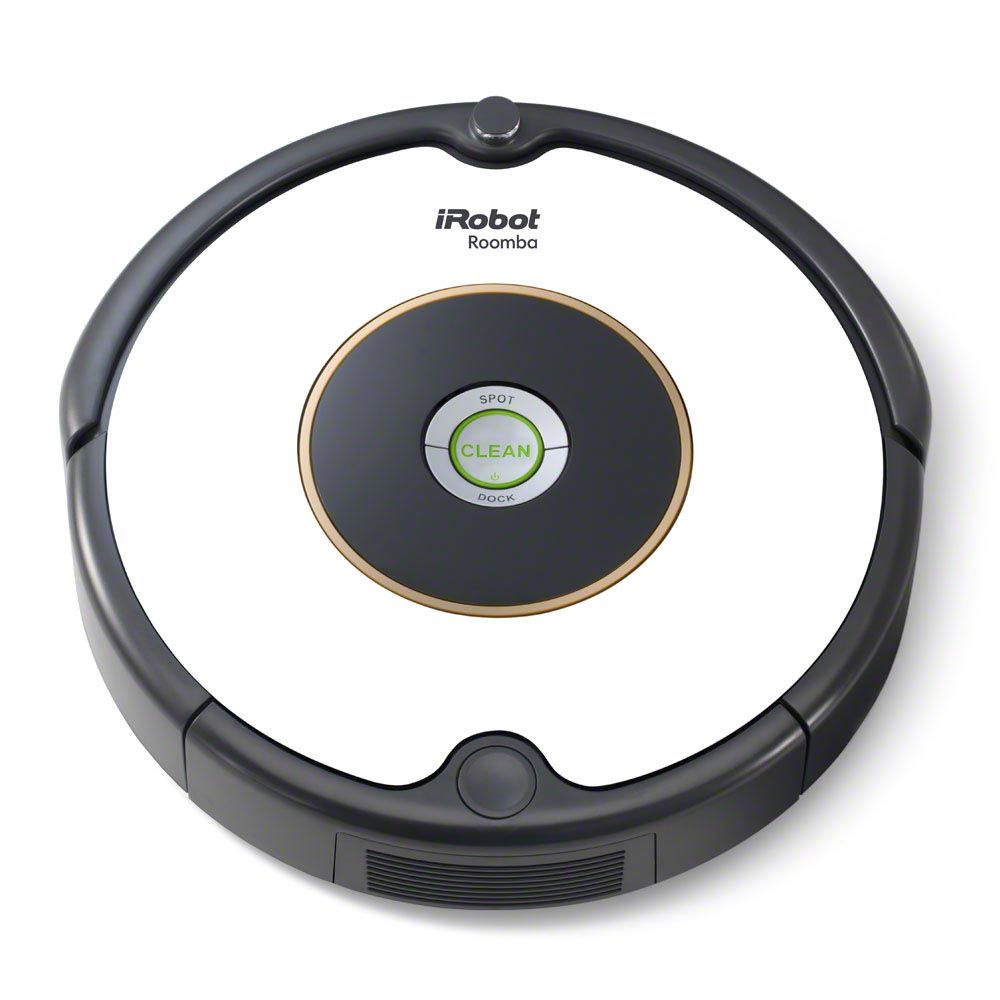
\includegraphics[scale=0.15]{bilder/implementierung/Roomba.jpg}\label{fig:roombaSub1} 
   \end{minipage}% 
   \hfill
\caption{Roomba 620 als Staubsaugerroboter. (Bild: Webshop des Herstellers, \url{http://shop.irobot.de/roomba-staubsstaubsaugerroboter-roomba-605/R605040.html?cgid=de\&lang=de_DE} (letzter Aufruf: 23. November 2016))}
\label{fig:roomba}
\end{figure}

Nachfolgend erfolgt die Vorstellung der Schnittstellendokumentation mit der Einführung in die bereitgestellten Kontrollmodi und der, für die Implementierung benötigten Befehle.


\subsection{Modi des iRoomba Create Open Interface (OI)}
Während der Benutzung des Roombas befindet sich dieser in einem der vier unterschiedlichen Kontrollmodi: Off, Passiv, Safe und Full \cite{IRobot2010}. Die Modi legen fest, welche Verhaltensweisen seitens des Roombas vorgesehen sind und wie auf eintreffende Befehle, (siehe Abschnitt~\ref{subsction:befehlsstruktur}) reagiert wird. Folgend werden die vier Modi des Roombas, wie in den Angaben des Herstellers beschrieben,
dargestellt \cite{IRobot2010}:
\begin{description}
\item[\enquote{Off}-Modus] Darin befindet sich der Roomba nach einem Batteriewechsel oder nach dem ersten Anschalten. Der Roomba erwartet in diesem Modus einen \enquote{Start}-Befehl (siehe Abschnitt~\ref{subsction:befehlsstruktur}) und wechselt nach Erhalten des Befehls in den \enquote{Passiv}-Modus.

\item[\enquote{Passiv}-Modus] Nach Erhalt eines \enquote{Start}-Befehls (siehe Abschnitt~\ref{subsction:befehlsstruktur}) wechselt der Roomba in diesen Modus. Hierbei können Sensordaten ausgelesen werden, jedoch sind keine Steuerbefehle für die vorhandenen Steuerkomponenten (Lautsprecher, Motoren, Leuchtdioden) möglich. 

\item[\enquote{Safe}-Modus] Der Safe-Modus bietet die gleiche Funktionalität wie der Passiv-Modus. Zusätzlich kann der Roomba dabei nun kontrolliert und gezielt gesteuert werden. Alle vorhandenen Befehle sind nun unter der Voraussetzung ausführbar, dass keines der folgenden sicherheitsrelevanten Ereignisse eingetreten ist: 
\begin{itemize}
\item Ein Abhang wird während der Vorwärts- oder Rückwärtsbewegung erkannt.
\item Ein Rad steckt fest.
\item Das Ladegerät ist angeschlossen und der Roomba wird geladen.
\end{itemize}
Tritt eines dieser sicherheitsrelevanten Ereignisse auf, werden alle Motoren umgehend gestoppt und der Roomba wird in den \enquote{Passiv}-Modus versetzt.

\item[\enquote{Full}-Modus] Durch das Senden eines \enquote{Full}-Befehls (siehe Abschnitt~\ref{subsction:befehlsstruktur}) erhält der Benutzer in vollem Umfang Zugang zu den Steuerkomponenten (Lautsprecher, Motoren, Leuchtdioden). Die sicherheitsrelevanten Ereignisse werden hierbei nicht überwacht.
\end{description}

\acl{abb}~\ref{fig:roombamodi} verdeutlicht die \og Kontrollmodi und ihre Zustandsänderungen in Abhängigkeit bestimmter Ereignisse.

\begin{figure}[ht]
  \centering
  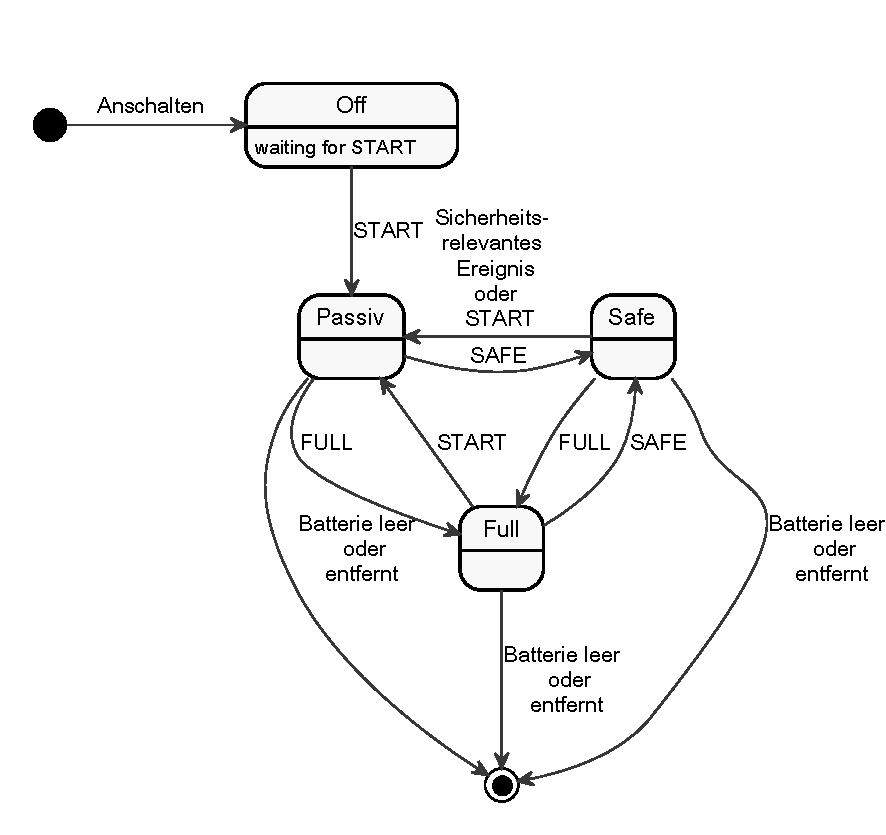
\includegraphics[width=0.6\textwidth]{bilder/implementierung/neuablauf2.pdf}
\caption{Darstellung der vier unterschiedlichen Kontrollmodi des Roombas und der Zustandsübergänge.}
\label{fig:roombamodi}
\end{figure}

\subsection{Befehlsstruktur des iRoomba Create Open Interface (OI)}
\label{subsction:befehlsstruktur}
Der Befehlsumfang, der durch das OI angeboten wird, bietet eine umfangreiche Interaktionsmöglichkeit mit den Sensoren und Steuerkomponenten des Roombas. Für die Implementierung des Softwareprototyps wurde nur eine kleine Anzahl der bereitgestellten Befehle verwendet. So wurde die Netzwerkkommunikation nur unilateral in Richtung des \acs{tps} genutzt. Auf das Auslesen der Senordaten des Roombas wurde aufgrund begrenzter Kapazitäten in Bezug auf die parallele bilaterale Kommunikation des angebrachten Access-Points verzichtet. Die nachfolgende Auflistung führt dadurch nur die für die Implementierung verwendeten Befehle auf. Für eine vollständige Auflistung sei auf die ausführlichen Angaben des Herstellers verwiesen (\vgl \cite{IRobot2010}). 
\begin{description}
\item \textbf{Modusbefehle}
\begin{itemize}
\item[\textsc{Start}] (Opcode: 128) (Datenbytes: 0)
\item[\textsc{Safe}] (Opcode: 131) (Datenbytes: 0)
\item[\textsc{Full}] (Opcode: 132) (Datenbytes: 0)
\item[\textsc{Dock}] (Opcode: 143) (Datenbytes: 0)
\end{itemize}
\item \textbf{Fahrbefehle}
\begin{itemize}
\item [\textsc{Drive}] (Opcode: 137) (Datenbytes: 4)
\item [\textsc{Drive} \textsc{Direct}] (Opcode: 145) (Datenbytes: 4)
\end{itemize}
\end{description}
Jeder OI-Befehl beginnt mit einem Ein-Byte großen Befehlsopcode, der den gewünschten Befehl codiert. In Abhängigkeit des Befehlsopcodes werden zusätzlich ein oder mehrere weitere Datenbytes als Argument des Befehls benötigt.
\begin{equation*}
\noindent \color{black} \underbrace{\textbf{|OPCODE|}}_{\substack{\text{Befehlsauswahl}}}\hfill \color{black}\underbrace{\textbf{|Datenbyte 1|}\hfill \textbf{|Datenbyte 2|} \hfill \textbf{|Datenbyte 3|}\hfill \textbf{|Datenbyte 4|}}_{\substack{\text{Variable Anzahl der Datenbytes in Abhänigkeit des Befehlsopcods}}} \hfill 
\end{equation*}

Viele Befehle, wie beispielsweise der oben bereits genannte \textsc{Start}-Befehl~(Opcode:~128), benötigen keine zusätzlichen Datenbytes. Dies trifft auch auf die Gruppe der Modus-Befehle, wie beispielsweise auf den \textsc{Safe}-Befehl~(Opcode:~131), der den Roomba in den \enquote{Safe}-Modus versetzt, oder auf den \textsc{Full}-Befehl~(Opcode:~132), womit der Roomba in den \enquote{Full}-Modus wechselt, zu.

Für die Umsetzung der diskreten und kontinuierlichen Steuerung wurden zwei unterschiedliche Steuerungsbefehle verwendet. Für die diskrete Steuerung bot sich die Funk\-tions\-weise des \textsc{Drive}-Befehls~(Opcode:~137) an und bei der kontinuierlichen Steuerung wurde die Funktion des \textsc{Drive Direct}-Befehls~(Opcode:~145) verwendet, deren allgemeine Beschreibung hier nun folgen. Die konkrete Anwendung folgt in den Abschnitten~\ref{subsection:diskSt} \bzw \ref{subsection:kontSt}.

\subsubsection{\textsc{DRIVE}-Befehl (Opcode:~137)}
Für die Steuerung mittels \textsc{Drive}-Befehls (Opcode:~137) wurde die Ansteuerung der beiden Radmotoren des Roombas durch die Angabe zweier Argumente realisiert (Geschwindigkeit, Radius), \vgl Listing~\ref{lst:drive}.
Hierbei erfolgte die Steuerung durch die Angabe einer durch zwei Bytes codierten \textit{Geschwindigkeit}, im Bereich von -500 mm/s bis \mathplus 500 mm/s, kombiniert mit der Angabe eines, durch weitere zwei Bytes codierten \textit{Radius} im Bereich von -2000 mm bis \mathplus 2000 mm. Daraus ergibt sich für den \textsc{Drive}-Befehl die allgemeine \textit{sequenzielle Struktur} des Befehls:
\begin{equation*}
\begin{split}
\underbrace{\underbrace{\text{|137|}}_{\substack{\text{\text{1 Byte}}}}}_{\substack{\text{\textsc{opcode}}}} \underbrace{\underbrace{\text{|höherwertiges Byte|}}_{\substack{\text{1 Byte}}} \underbrace{\text{|niederwertiges Byte|}}_{\substack{\text{1 Byte}}}}_{\substack{\text{\textsc{Geschwindigkeit}}}} \underbrace{\underbrace{\text{|höherwertiges Byte|}}_{\substack{\text{1 Byte}}} \underbrace{\text{|niederwertiges Byte|}}_{\substack{\text{1 Byte}}}}_{\substack{\text{\textsc{Radius}}}}
\end{split}
\end{equation*}

Anhand der allgemeinen Struktur des \textsc{Drive}-Befehls kann man erkennen, dass zusätzlich zum Opcode-Byte vier weitere Datenbytes notwendig sind, die als zwei vorzeichenbehaftete 16-Bit-Zahlen in Zweierkomplementdarstellung vorliegen. Dabei erkennt man ferner, dass eine Big-Endian-Byte-Reihenfolge vorgesehen ist und dass das höchstwertige Byte zuerst angegeben werden muss. Ist es beispielsweise vorgesehen, den Roomba mit einer Geschwindigkeit von 200 mm/s in Rückwärtsrichtung (Geschwindigkeit mit negativem Vorzeichen) zu bewegen und gleichzeitig in einem Radius von 500 mm zu drehen, ergibt sich folgende Bytesequenz des Befehls \cite{IRobot2010}:
\begin{beispiel}{Beispielsequenz eines \textsc{Drive}-Befehls: [137] [255] [56] [1] [244]} \\
\centering
\(
\underbrace{\color{orange}\underbrace{\underbrace{\text{\textsc{ Opcode }}}_{\substack{\text{\textsc{Drive}}}}}_{\substack{\text{\textsc{|137|}}}}
\color{blue}\underbrace{\underbrace{\underbrace{\text{\textsc{ Geschwindigkeit }}}_{\color{blue}\substack{\text{-200 mm/s}}}}_{\color{blue}\substack{hex FF38}}}_{\color{blue}\substack{\underbrace{hex FF}_{\substack{|255|}}\underbrace{hex 38}_{\substack{|56|}}}}\color{black}\underbrace{\underbrace{\underbrace{\text{\textsc{ Radius }}}_{\substack{\text{500 mm}}}}_{\substack{hex 01F4}}}_{\substack{\underbrace{hex 01}_{\substack{|1|}}\underbrace{hex F4}_{\substack{|244|}}}}} \)\\
\( [137] [255] [56] [1] [244] \)
\label{exa:drive}
\end{beispiel}

Der \textsc{Drive}-Befehl stellt für einige Bewegungsrichtungen,- wie die Drehung nach links oder rechts,- und die Geradausfahrt in Vorwärts- und Rückwärtsrichtung,- spezielle Werte des Radius-Parameters bereit (\vgl~\cite{IRobot2010}):

\begin{itemize}
  \item Gerade = 32768 oder 32767 = hex 8000 oder 7FFF (\vgl~Listing~\ref{lst:vorruck})
  \item Drehung nach rechts = hex FFFF (\vgl~Listing~\ref{lst:rotrechts})
  \item Drehung nach links = hex 0001 (\vgl~Listing~\ref{lst:rotlinks})
\end{itemize}

Der \textsc{Drive}-Befehl kann, wie oben erwähnt, nur während der Ausführung im \enquote{Safe}- oder \enquote{Full}-Modus verwendet werden. Das \og Beispiel zeigt die allgemeine Befehlsstruktur des von der OI bereitgestellten \textsc{Drive}-Befehls~(Opcode:~137). 

\subsubsection{\textsc{DRIVE} \textsc{DIRECT}-Befehl (Opcode:~145)}
Der \textsc{Drive}~\textsc{Direct}-Befehl (Opcode:~145) unterscheidet sich zum \og \textsc{Drive}-Befehl dahingehend, dass die Ansteuerung der einzelnen Radsteuermotoren für jedes Rad einzeln möglich ist, \vgl auch Listing~\ref{lst:drivedirect}. Dadurch lässt sich die für die kontinuierliche Steuerung notwendige differenzierte kontinuierliche geschwindigkeits- und richtungsabhängige Befehlscodierung in einem einfachen Algorithmus implementieren, siehe Abschnitt~\ref{subsection:kontSt}. Es folgt die allgemeine \textit{sequenzielle Struktur} des \textsc{Drive}~\textsc{Direct}-Befehls~(Opcode:~145):
\begin{equation*}
\begin{split}
\underbrace{\underbrace{\text{|145|}}_{\substack{\text{\text{1 Byte}}}}}_{\substack{\text{\textsc{opcode}}}} \underbrace{\underbrace{\text{|höherwertiges Byte|}}_{\substack{\text{1 Byte}}} \underbrace{\text{|niederwertiges Byte|}}_{\substack{\text{1 Byte}}}}_{\substack{\text{\textsc{Geschwindigkeit rechtes Rad}}}} \underbrace{\underbrace{\text{|höherwertiges Byte|}}_{\substack{\text{1 Byte}}} \underbrace{\text{|niederwertiges Byte|}}_{\substack{\text{1 Byte}}}}_{\substack{\text{\textsc{Geschwindigkeit linkes Rad}}}}
\end{split}
\end{equation*}

Anhand seiner allgemeinen Struktur des \textsc{Drive} \textsc{Direct}-Befehls erkennt man, dass genau wie beim \textsc{Drive}-Befehl zusätzlich zum Opcode-Byte vier weitere Datenbytes benötigt werden. Hierbei handelt es sich auch um zwei 16-Bit Zahlen in Zweierkomplementärdarstellung und in Big-Endian-Byte-Reihenfolge.
Ein konkretes Beispiel verdeutlicht die Nutzung des \textsc{Drive} \textsc{Direct}-Befehls:

\begin{beispiel}{Beispielsequenz eines \textsc{Drive} \textsc{Direct}-Befehls: [145] [0] [200] [0] [200]} \\
%\textbf{[137] [255] [56] [1] [244]} \\ 
\centering
\(\color{orange}\underbrace{\text{|145|}}_{\substack{\text{\textsc{Drive}\textsc{Direct }}}}\color{blue}\underbrace{\underbrace{\underbrace{\text{|0|}}_{\substack{\text{hex 00}}} \underbrace{\text{|200|}}_{\substack{\text{hex C8}}}}_{\substack{= \text{200 mm/s}}}}_{\substack{\text{\textsc{Geschwindigkeit rechtes Rad }}}} \color{black}\underbrace{\underbrace{\underbrace{\text{|0|}}_{\substack{\text{hex 00}}} \underbrace{\text{|200|}}_{\substack{\text{hex C8}}}}_{\substack{= \text{200 mm/s}}}}_{\substack{\text{\textsc{Geschwindigkeit linkes Rad }}}}\)
\label{exa:driveDirect}
\end{beispiel}

Die erzeugte Bewegung der Befehlssequenz im Beispiel~\ref{exa:driveDirect} entspräche einer Fahrt mit einer Geschwindigkeit von 200 mm/s geradeaus, da beide Motoren dieselbe Geschwindigkeit umsetzen.

Die Umsetzung des \textsc{Drive} \textsc{Direct}-Befehls kann ebenfalls nur während der Ausführung im \enquote{Safe}- oder \enquote{Full}-Modus erfolgen. 

Nachfolgend wird auf die konkrete Umsetzung der beschriebenen Befehle (\textsc{Drive}-Befehl~(Opcode:~137), \textsc{Drive} \textsc{Direct}-Befehl (Opcode:~145)) für die Steuermodelle eingegangen und die Anwendung der Befehle nochmals verdeutlicht.

\section{Umsetzung der Robotersteuerung des Prototyps}
\label{subsection:robotsteuerung}
Nachdem die Befehlsstruktur der Schnittstelle des Roombas im vorherigen Abschnitt beschrieben wurde, folgt nun die konkrete Anwendung der Befehle im Rahmen der beiden Steuerungsmethoden. 

\subsection{Umsetzung der diskreten Steuermethode}
\label{subsection:diskSt}
Wie bereits in Abschnitt \ref{subsection:gestDisk} beschrieben, wurden zur Umsetzung der diskreten Steuermethode vier Steuerelemente (vor, zurück, links, rechts) konzipiert.
Wird der Blick \bzw der \acs{por} des Benutzers in einem Bereich eines der Steuerelemente gelenkt, so wird der entsprechende Befehl an den mobilen Roboter gesendet. Hierbei wird beispielsweise durch das \enquote{vor}- Steuerelement das Signal einer translationalen Bewegung in Vorwärtsrichtung in der aktuellen Geschwindigkeit an den mobilen Roboter gesendet. Durch das Steuerelement \enquote{zurück} entsprechend in Rückwärtsrichtung. Verlässt der \acs{por} des Benutzers den Bereich des Steuerelements, wird dementsprechend kein weiteres Signal gesendet und das \acs{tps} verbleibt an der aktuellen Position. Wird durch eine Blickgeste das \enquote{links}- oder \enquote{rechts}-Steuerelement ausgewählt, so wird ein Befehl zur Rotation nach links oder nach rechts an den mobilen Roboter gesendet. Eine translationale Bewegung findet hierbei nicht statt, der mobile Roboter dreht sich an der aktuellen Position. Dabei wird beim Verlassen der Blickbewegung des jeweiligen Steuerelements auch die entsprechende Rotationsbewegungsbewegung gestoppt. Durch diese Art der Steuerung werden durch alternierende Rotation und Translationsbewegungen jegliche Positionen auf dem Feld erreicht und die Voraussetzungen für eine Umsetzung der Parcoursbewältigungsaufgabe sind prinzipiell gegeben. Wie bereits im Abschnitt~\ref{subsction:befehlsstruktur} dargelegt, wurde zur Realisierung der Steuerkomponenten der diskreten Steuerung der Befehl \textsc{Drive} verwendet. Hierbei wurde jede Steuerkomponente (vor, zurück, links, rechts) für die beabsichtigte Bewegungsrichtung durch die feste Zuteilung der Befehlsparameter (Geschwindigkeit, Radius) für eine der vier möglichen Bewegungen zugewiesen. Die Geschwindigkeit des mobilen Roboters ließ sich in den allgemeinen Systemeinstellungen für die diskrete Steuerung festlegen. Zur Erzeugung der Bewegungsrichtungen in einer Geschwindigkeit von 200 mm/s wurden folgende Befehlssequenzen erzeugt: 
\begin{description}
\item [Vorwärts:] [137] [0] [200] [128] [0]
\item [Rückwärts:] [137] [255] [56] [128] [0]
\item [Drehung nach rechts:] [137] [0] [200] [255] [255]
\item [Drehung nach links:] [137] [0] [200] [0] [1]
\end{description}

Die Realisierung des \enquote{Panikschalters} für die diskrete Steuerungsmethode wurde dadurch ermöglicht, dass eine Steuerung des mobilen Roboters nur durch das jeweilige Betätigen einer Steuerkomponente erfolgte. Es war ausreichend, den \acs{por} in einen der Bereiche ohne Steuerelemente zu lenken, um im Notfall keine Steuersignale zu senden. Ferner ist es möglich, durch einen Lidschluss die Steuerung zu pausieren und sich im Blickbereich \enquote{umzusehen}, bevor man die Steuerung mittels eines erneuten Lidschlusses erneut startet. 

\begin{comment}
Programmiertechnisch wurde dies mittels folgender Implementierungen umgesetzt. Die Methoden sind von der ..., des Projekts Hacking Roomba abgeleitet \cite{Kurt2007}.
\lstinputlisting[language=java, numbers=left, firstline=336, lastline=342,frame=single,breaklines=true, style=myCustomJavaStyle, caption={Vorwärts- und Rückwertsbewegung}, label=lst:vorruck]{code/ARoomba.java}

Wie in Listing \ref{lst:vorruck} dargestellt wird die Vorwärts  \bzw Rückwärtsbewegung durch das Vorzeichen der Geschwindigkeit definiert. Die Angabe des Parameters \(0x8000 = [128] [0]\) des Radius definiert wie bereits in Abschnitt \ref{subsction:befehlsstruktur} beschrieben die Fahrt geradeaus. Die dargestellten Fallunterscheidungen dienen der Limitation auf die maximal positive und negative Geschwindigkeit von 500 mm/s.

\lstinputlisting[language=java, numbers=left, firstline=321, lastline=323,frame=single,breaklines=true, style=myCustomJavaStyle, caption={Rotationsbewegung in Uhrzeigersinn}, label=lst:rotrechts]{code/ARoomba.java}

\lstinputlisting[language=java, numbers=left, firstline=311, lastline=313,frame=single,breaklines=true, style=myCustomJavaStyle, caption={Rotationsbewegung entgegen des Uhrzeigersinn},label=lst:rotlinks]{code/ARoomba.java}

Wie in Listing \ref{lst:rotrechts} und \ref{lst:rotlinks} dargestellt werden die Rotationsbewegungen durch Angabe des Parameters \(\text{0xffff = [255] [255]}\) und \(\text{0x0001 = [0] [1]}\) des Radius definiert wie auch bereits in Abschnitt \ref{subsction:befehlsstruktur} beschrieben wurde. Somit wird bei der Betätigung der Steuerelemente \enquote{Rechts} und \enquote{Links} der in Listing \ref{lst:rotrechts} und \ref{lst:rotlinks} Code aufgerufen.

\lstinputlisting[language=java, numbers=left, firstline=390, lastline=394,frame=single,breaklines=true, style=myCustomJavaStyle, caption={Drive-Befehl},label=lst:drive]{code/ARoomba.java}

Listing \ref{lst:drive} zeigt die Umsetzung des \textsc{Drive}-Befehls in Java. Die Umsetzung eines Stoppbefehls ist in Listing \ref{lst:stop} gezeigt. Hierbei wird eine Befehl mit der Geschwindigkeit Null und dem Radius Null erzeugt.

\lstinputlisting[language=java, numbers=left, firstline=177, lastline=179,frame=single,breaklines=true, style=myCustomJavaStyle, caption={Stop-Befehl},label=lst:stop]{code/ARoomba.java}
\end{comment}

\subsection{Umsetzung der kontinuierlichen Steuermethode}
\label{subsection:kontSt}
Im Vergleich zur diskreten Steuerung wurden, wie bereits \og, mittels der kontinuierlichen Steuerung keine fest zugewiesenen Befehle erzeugt. Vielmehr sollte es für den Benutzer möglich sein, durch entsprechende Augenpositionierung die Geschwindigkeit und die Richtung während der Fahrt flexibel zu variieren. Möglich ist dies durch den beschriebenen \textsc{Drive} \textsc{Direct}-Befehl. Hierbei wird der \acs{por} des Benutzers durch eine Umrechnung in die Geschwindigkeit beider Radmotoren übersetzt. Eine Richtungsänderung der Bewegung kann, wie \og, durch unterschiedliche Geschwindigkeiten der beiden Radmotoren erzielt werden.

Zur Verdeutlichung der Geschwindigkeitsberechnung der Radmotoren während unterschiedlicher Positionen des \acs{por} sei auf die grafischen Beispiele in \acs{abb}~\ref{fig:allkontModus} verwiesen.

\begin{figure}[ht]
   \begin{minipage}[b]{.5\linewidth} 
      \centering 
      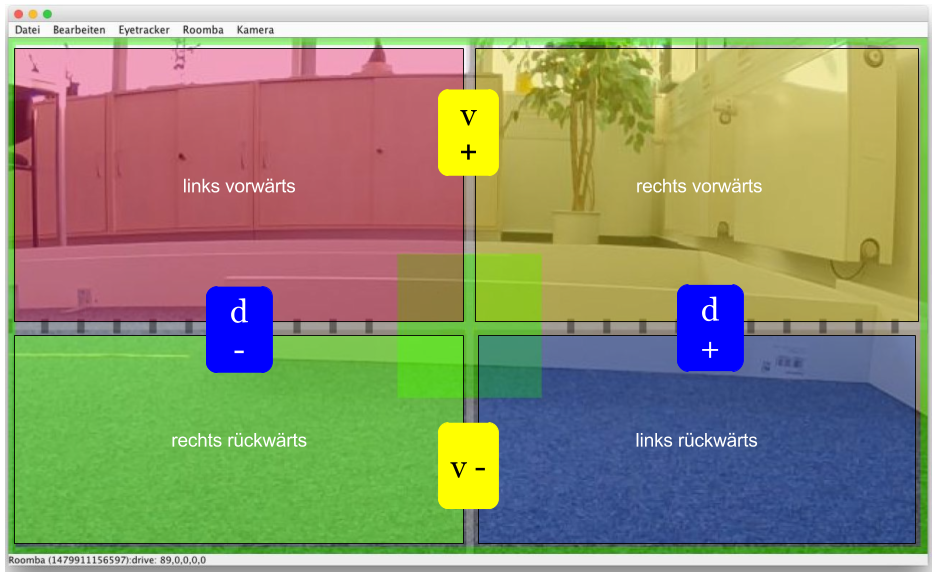
\includegraphics[width=1\textwidth]{bilder/implementierung/richtungen.png} 
      \subcaption{Neutrale Zone}\label{fig:1} 
   \end{minipage}% 
   \hfill
   \begin{minipage}[b]{.5\linewidth} 
      \centering 
      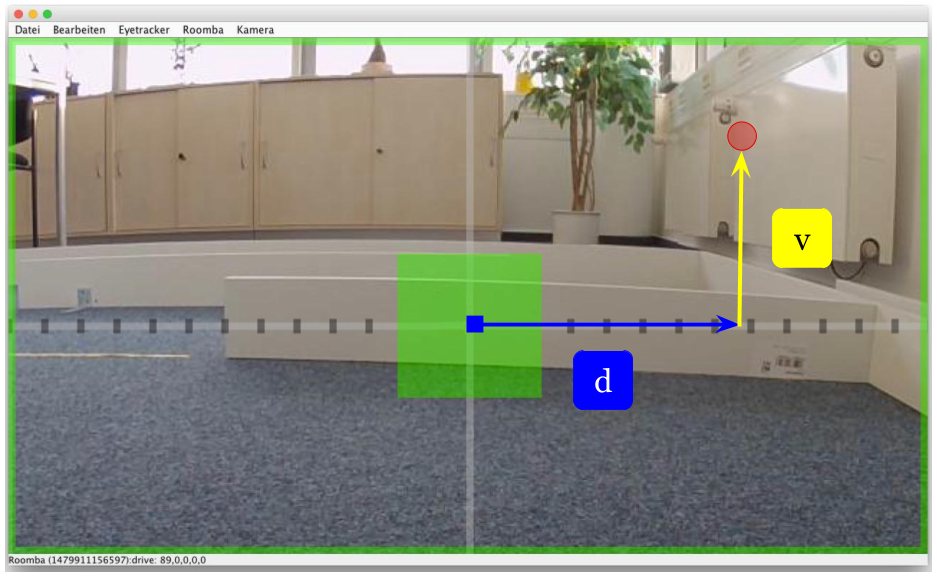
\includegraphics[width=1\textwidth]{bilder/implementierung/rechtsDrive.png} 
      \subcaption{Rechts Vorne}\label{fig:2} 
   \end{minipage}%
   \hfill
   \begin{minipage}[b]{.5\linewidth} 
      \centering 
      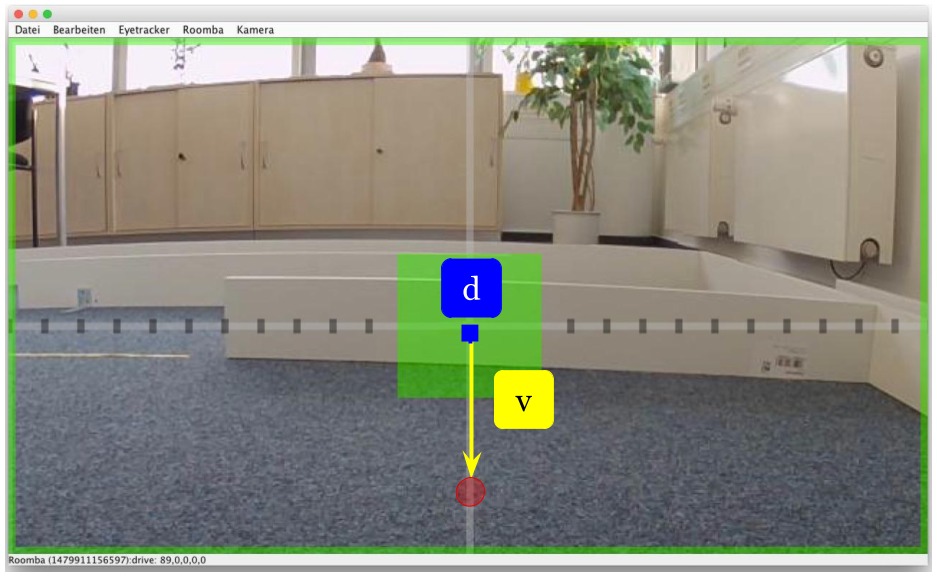
\includegraphics[width=1\textwidth]{bilder/implementierung/ruckDrive.png} 
      \subcaption{Rückwärts}\label{fig:3} 
   \end{minipage}%
   \hfill
   \begin{minipage}[b]{.5\linewidth} 
    \centering 
	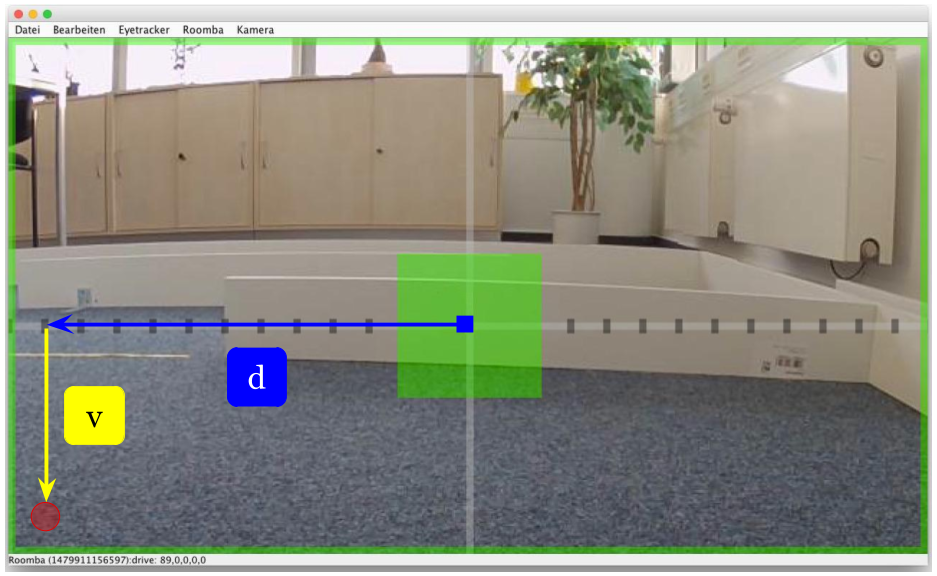
\includegraphics[width=1\textwidth]{bilder/implementierung/linksDrive.png} 
      \subcaption{Links hinten}\label{fig:4} 
   \end{minipage}%
   \hfill
   \caption{Ausgewählte Steuersignale der kontinuierlichen Steuermethode. Blickbewegung in y-Richtung (in Relation zum Mittelpunkt des Koordinatenkreuzes) als $v$ bezeichnet. Blickbewegung in x-Richtung (in Relation zum Mittelpunkt des Koordinatenkreuzes) als $d$ bezeichnet. \textbf{\subref{fig:1}}~zeigt die Wertentwicklung der beiden Variablen in Abhängigkeit der Blickbewegung.}\label{fig:allkontModus} 
\end{figure} 

Der \enquote{Ausschlag} der Blickbewegung in y-Richtung (in Relation zum Mittelpunkt des Koordinatenkreuzes), in \acs{abb}~\ref{fig:allkontModus} als $v$ bezeichnet, definiert die Geschwindigkeit der Radmotoren. Die Blickbewegung innerhalb der oberen Hälfte des Blickfeldes, getrennt durch die Abszisse des Koordinatenkreuzes, erzeugt eine Vorwärtsbewegung der Räder des \acs{tps}. Die Blickbewegung innerhalb der unteren Hälfte des Blickfeldes dementsprechend eine Rückwärtsbewegung. In Abhängigkeit des Abstandes in x-Richtung (in Relation zum Mittelpunkt des Koordinatenkreuzes), in \acs{abb}~\ref{fig:allkontModus} als $d$ bezeichnet, werden nach den folgenden Formeln die einzelnen Radgeschwindigkeiten (rechtes Rad~$V_{r}$, linkes Rad~$V_{l}$) berechnet und somit Richtungsänderungen ermöglicht:
\begin{equation}
\begin{split}
V_{r} = v - d \\\
V_{l} = v + d
\end{split}
\label{eq:formel}
\end{equation}

Wird der Blick beispielsweise in den rechten oberen Bereich des Blickfeldes gerichtet (gelber Bereich, \vgl \acs{abb}~\ref{fig:allkontModus}), resultiert nach Gleichung \ref{eq:formel} eine Reduktion des positiven Geschwindigkeitsfaktors~$v$ des rechten Rades~$V_{r}$ um den positiven Faktor~$d$. Gleichzeitig addiert sich zum Geschwindigkeitsfaktor~$v$ des linken Rades~$V_{l}$ der positive Faktor~$d$ hinzu. Die resultierende Bewegung ist demnach eine nach vorn und rechts gerichtete Bewegung des \acs{tps}.

Für den oben links gelegenen Bereich (roter Bereich, \vgl~\acs{abb}~\ref{fig:allkontModus}) ergibt sich aufgrund der Gleichung und des negativen Faktors~$d$ entsprechend die Bewegung des \acs{tps} nach links vorn.  Blickbewegungen, beispielsweise in den unteren linken Blickbereich (grüner Bereich, \vgl~\acs{abb}~\ref{fig:allkontModus}), führen nach Formel~\ref{eq:formel} aufgrund des jetzt negativen Faktors~$v$ und des negativen Faktor~$d$ zu einer schnelleren Rückwertsdrehung des linken Rades~$V_{l}$ im Vergleich zum rechten Rades~$V_{r}$ und dadurch zu einer nach rechts gerichteten Rückwärtsbewegung. Hierdurch wird ersichtlich, dass durch die vorkommenden Vorzeichen der Gleichung~\ref{eq:formel} und die Vorzeichen der Faktoren~$v$~und~$d$ ein Wechsel der Drehrichtung während eines vertikalen Blickwechsels selben Seite des Blickfeldes resultiert. Anders als vielleicht intuitiv angenommen, muss, um eine Bewegung des \acs{tps} quasi rückgängig zu machen, eine diagonale Blickbewegung ausgeführt werden und nicht - wie vielleicht vermutet - eine vertikale. Dies wäre lediglich für den Fall einer Umkehr einer Vorwärts- \bzw Rückwärtsbewegung sinnvoll.


Die Umsetzung des \enquote{Panikschalters} wurde dadurch realisiert, dass der mobile Roboter nur außerhalb der \enquote{Neutralzone} Steuersignale erhält. Ferner war es möglich, im Bereich der Neutralzone durch einen Lidschluss die Steuerung der kontinuierlichen Methode zu pausieren und sich im Blickbereich \enquote{umzusehen}, bevor man die Steuerung mittels eines erneuten Lidschlusses im Bereich der Neutralzone erneut starten konnte. Dadurch sollte eine unbeabsichtigte Steuerung vermieden werden. 


\section{Eyetracking-System}
\label{section:eyetrackingI}
Im Rahmen der Steuerung des \acs{tps} im vorliegenden Softwareprototyp erfolgte die Erkennung der Augengesten durch das bereits in der Vorarbeit von Eidam et al. \vgl~\cite{Eidam2015} vorgestellte Eyetracking-System \iV des Unternehmens \acf{smi}, siehe \acs{abb}~\ref{fig:device}. Die präzise Erkennung der Augengesten ist im Hinblick auf die erfolgreiche Steuerung des \acs{tps} entscheidend. Der folgende Abschnitt orientiert sich vornehmlich an den Beschreibungen von Eidam (2015) \vgl~\cite{Eidam2015} und stellt die benötigten Komponenten genauer dar.

\subsection{\iV System und \acf{red}}
Das vorgestellte \acs{red} \acl{et} ermöglicht eine kontaktlose Detektion der Augenbewegungen einer Testperson, da es sich um ein stationäres \acs{et} handelt \cite[S.165]{SMI2011}. Das \acs{et} benutzt zwei Infrarot-LED\footnote{Abkürzung für \textit{light-emitting diode} oder \textit{lichtemittierende Diode}}-Quellen zur Erzeugung der für die Detektion benötigten Cornealreflexe \cite[S.22]{SMI2011} (\vgl Ausführungen in Abschnitt~\ref{section:eyeMet}).

Zusätzlich zum \acs{et} besteht das von \acs{smi} bereitgestellte \iV System noch aus einer \acf{wo} und einem stimuluspräsentierenden PC (SP) \cite[S.23]{SMI2011}.
Ein großer Vorteil des \iV Systems besteht in der Bereitstellung einer Middleware (\iV), die für andere Computer oder Anwendungen die Möglichkeit eröffnet, durch eine Systemschnittstelle mit dem \iV zu interagieren und Daten untereinander auszutauschen \cite{SMI2011}. Diese Middleware ermöglicht mittels Imageprocessing die in Echtzeit ablaufende Analyse der Pupillendetektion, die Entfernung von Artefakten und die Berechnung der \acs{por} basierend auf dem in Abschnitt \ref{section:eyeMet} beschriebenen \enquote{Dark-Pupil}-Verfahren zur Erkennung der Augengeste.  
Das \iV System umfasst hierbei folgende Komponenten, die in der \acs{abb}~\ref{fig:eyetracker} dargestellt sind:

\begin{itemize}
\item \iV \acf{wo} 
\item \acf{spb}
\item \acf{et}
\end{itemize}

\begin{figure}[ht]
\begin{center}
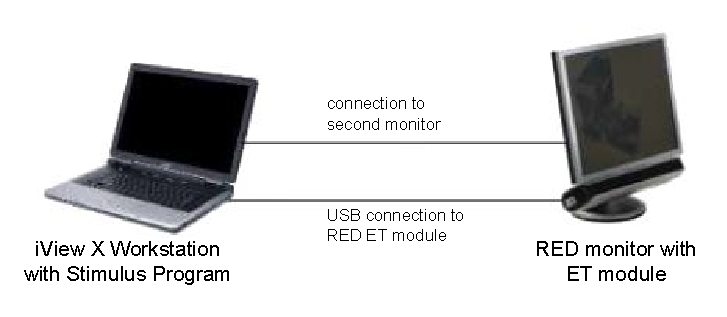
\includegraphics[width=0.7\textwidth]{bilder/implementierung/blick.pdf}
\end{center}
\caption{Die \iV \acf{wo} als Laptop in Verbindung mit dem \acf{spb} und dem \acf{et}. Die \iV Workstation beinhaltet die vorinstallierte Middelware, die zur Kommunikation mit dem Softwareprotyp dient \cite{SMI2011}. (Bild: aus \cite[S.143]{SMI2011})}
\label{fig:eyetracker}
\end{figure}

Nachfolgend wird die Middlewaredokumentation mit der Einführung in die Befehlsstruktur der bereitgestellten Systemschnittstelle vorgestellt.

\subsection{Systemschnittstelle der Middleware (\iV)}
Die Programmierschnittstelle beinhaltet eine Reihe von Befehlen, die es ermöglichen, die Middelware (\iV) durch andere Computer respektive durch den Softwareprototyp zu steuern. Die Kommunikation mit der \iV-Software findet hierbei mittels einer auf \acf{udp} basierenden Netzwerkkommunikation statt \cite[S.439]{SMI2011}. Zur Kommunikation werden nicht alle angebotenen Befehle verwendet. Es erfolgt eine Fokussierung auf die zur Implementierung des Prototyps verwendeten Befehle. Der allgemeine Aufbau eines Befehls besteht aus einer Stringfolge und beginnt bei allen Befehlen mit einer drei Zeichen großen Stringfolge \enquote{ET\_}, gefolgt von einer weiteren, welche die beabsichtigte Aktion spezifiziert \cite[S.484]{SMI2011}\cite{Eidam2015}. In Abhängigkeit der spezifizierten Befehle werden schließlich weitere durch Stringfolgen codierte Parameter angegeben. Die nachfolgende Auflistung führt nur die für die Implementierung verwendeten Befehle aus der Gruppe der Kalibrierungs- und der Datenoutputbefehle auf. Für eine vollständige Auflistung der möglichen Befehle sei auf die ausführlichen Angaben des Herstellers verwiesen (\vgl \cite[484 ff.]{SMI2011}).

\paragraph{Kalibrierungsbefehle}
\begin{itemize}
\item \textbf{ET\_CAL <Punkte> <Binokular Modus>} beginnt die Kalibrierung durch Angabe der zur Kalibrierung notwendigen Punkte durch den Parameter <Punkte>. Mögliche Werte sind (\enquote{2},\enquote{5},\enquote{9},\enquote{13}). Optionaler Parameter nur während der Nutzung des binokularen Modus, wobei \enquote{1} = rechtes Auge, \enquote{2} = linkes Auge repräsentiert \cite[S.489-490]{SMI2011}.
\item \textbf{ET\_CSZ <Breite> <Höhe>} legt die Größe der Kalibrierungsfläche fest, wobei die Fläche durch die Angabe der Pixel mithilfe der Parameter <Breite> und <Höhe> definiert werden \cite[S.493-494]{SMI2011}.
\item \textbf{ET\_PNT <Punktnummer> <X> <Y>} setzt die Koordinaten eines Punktes, charakterisiert durch die <Punktnummer> (Werte zwischen 1 bis 13, siehe Abbildung) und die X- und Y-Koordinate durch die Parameter <X> und <Y> auf dem Bildschirm in Pixel fest \cite[S.503-504]{SMI2011}.
\item \textbf{ET\_CHG <Punktnummer>} signalisiert den Wechsel zum nächsten Kalibierungspunkt durch Angabe der <Punktnummer> \cite[S.490-491]{SMI2011}.
\item \textbf{ET\_ACC} signalisiert das Akzeptieren des aktuellen Kalibierungspunktes und wechselt zum nächsten Kalibrierungspunkt. Dieser Befehl benötigt keinen Parameter \cite[S.487]{SMI2011}.
\item \textbf{ET\_FIN} signalisiert die abgeschlossene Kalibrierung. Dieser Befehl benötigt keine Angabe eines Parameters \cite[S.497]{SMI2011}.
\end{itemize}
\paragraph{Datenoutputbefehle}
\begin{itemize}
\item \textbf{ET\_FRM <Parameterstring : \%TS: \%SX \%SY>} legt das Datenouputformat fest. <Parameterstring> unterscheidet sich in Abhängigkeit des gewählten Modus und setzt sich aus mehreren Teilstrings zusammen (für weitere Angaben siehe \cite[S.500]{SMI2011}):
\begin{itemize}
\item TS: timestamp in Millisekunden ($0 \dots 2^{64}/1000 ms$).
\item SX, SY: X \bzw Y- Wert der Blickposition in Pixel ($\pm 2^{31}$ Pixel).
\end{itemize}
Bei der Deaktivierung des binokularen Modus, wie im Prototyp verwendet, erfolgt trotzdem die Angabe von vier Parametern in der Form: linkes X-linkes Augen.

\item \textbf{ET\_STR} beginnt das kontinuierliche Datenstreaming. Dieser Befehl benötigt keine Angabe eines Parameters
\item \textbf{ET\_EST} beendet das kontinuierliche Datenstreaming. Dieser Befehl benötigt keine Angabe eines Parameters.
\item \textbf{ET\_SPL <Parameterstring : \%TS: \%SX \%SY>} spezifiziert erkannte Datenpunkte durch das im \emph{ET\_FRM}- Befehl festgelegte Format \cite[S.513-514]{SMI2011}).
\end{itemize}


\section{Umsetzung der Augengestenerkennung des Prototyps}
\label{section:augengestenerkennung}
Die Erkennung der Augengesten basiert auf dem von Eidam et al.~(2015, 2016) entwickelten Algorithmen und Prinzipien und wurde im Rahmen dieser Arbeit nahezu unverändert übernommen, \vgl~\cite{Eidam2016,Eidam2015}. Für den aktuellen Prototyp wurde lediglich die Erkennung einer Blickgeste basierend auf dem Algorithmus der Fixationsberechnung hinzugefügt. Damit werden vom vorliegenden Prototypen insgesamt fünf Augengesten erkannt: (1)~\textbf{Fixation}, (2)~\textbf{Blickgeste}, (3)~\textbf{Lidschluss}, (4)~\textbf{vertikale Augengeste}, (5)~\textbf{horizontale Augengeste}. Die \textbf{horizontale Augengeste} wurde wie bei Eidam et al. detektiert, erfüllt im vorliegenden Prototyp jedoch keine Funktion. 

Nachfolgend wird die Umsetzung der Augengesten nach Eidam et al. kurz wiederholend beschrieben \cite{Eidam2016,Eidam2015}.

Prinzipiell werden die vom Eyetracking-System stammenden Koordinaten in einem Koordinatenpuffer mit fester Kapazität geladen und mithilfe der folgenden Algorithmen und Methoden nach jedem Hinzufügen auf das Auftreten einer Augengeste hin untersucht \cite{Eidam2015}. 

\begin{description}
\item[Fixation] Die Registrierung der Fixation wird durch den Bewegungsumfang des \acs{por} berechnet. Bewegt sich der \acs{por} des Benutzers innerhalb eines \textit{definierten Zeitraums} und innerhalb eines \textit{begrenzten Pixelbereichs}, wird eine Fixation erkannt. Die Berechnung des begrenzten Pixelbereichs erfolgt dabei mittels des Algorithmus,~\(|maxX-minX|+|maxY-minY|\), der ein Maß für die Streuung der eingetroffenen Koordinaten ist und auch als Dispersion bezeichnet wird. Hierbei wird der maximale Abstand der detektierten x- und y- Koordinaten addiert und mit einem festgelegten Schwellenwert verglichen. Beim Unterschreiten des Schwellenwerts, also einer Bewegung innerhalb des geforderten Pixelbereichs, wird eine Fixation ausgelöst.
Die Anzahl der zu vergleichenden Koordinaten nach der \og Formel richtet sich nach der gewählten Verweildauer und der Abtastrate des Eyetrackers. Letztere beträgt für den verwendeten Eyetracker 60 Hz. Bei einer Verweildauer von \zB 1000 ms wären dies somit 60 Koordinaten, die durch den \og Algorithmus verglichen werden \cite{Eidam2015}. Durch den Schwellenwert der Dispersion ist es möglich, die Sensitivität\footnote{Grad der Ansprechbarkeit} der Fixation anzupassen \cite[S.295]{SMI2011}. Je näher der Schwellwert dem Wert null liegt, desto exakter musste fixiert werden, um eine Fixationsgeste auszulösen.

\item[Blickgeste] Analog zur Fixationsgeste erfolgt die Umsetzung der Blickgeste auf dem gleichen \og Algorithmus der Dispersionsberechnung. Hierbei unterscheidet sich lediglich die Anzahl der zu vergleichenden Koordinaten. Dies resultiert aus der verkürzten Verweildauer von 100 ms für die Blickgeste. Der Koordinatenpuffer nimmt bei einer Abtastrate von 60 Hz für den Eyetracker 6 Koordinaten und vergleicht diese nach dem \og Prinzip. Damit können pro Sekunde 10 Blickgesten generiert werden.

\item[Lidschluss] Während eines Lidschlusses kommt es aufgrund der kurzzeitigen Verdeckung der Pupille durch das Ober- und Unterlied zu einer temporären Unterbrechung des Koordinatenstroms, wodurch nur Nullwerte vom Eyetracker gesendet werden \cite{Eidam2015}. Dieses passiert auch, wenn der Blick des Benutzers vom Eyetracking-System nicht mehr erkannt wird, beispielsweise weil der Blick vom \acs{et} abgewendet wird. Deshalb muss hier eine Obergrenze definiert werden muss, um nicht jede Blickabwendung zu definieren. Auch zur Unterscheidung eines willkürlichen Lidschlusses als Steuersignal von einem reflexartigen Lidschluss muss eine Ober- \bzw Untergrenze festgelegt werden. Diese Grenzen wurden, wie bei Eidam et al., im Bereich von 250 ms für die untere Grenze und bis 500 ms für die obere Grenze definiert. So werden bei der Abtastrate von 60 Hz mindestens 15 Nullwerte als unterste Grenze benötigt, um eine Lidschlussgeste zu detektieren. Bei einer Anzahl von über 30 Koordinaten ist die Obergrenze erreicht und die Lidschlussgestendetektion wird abgebrochen \cite{Eidam2015}.

\item[Horizontale und vertikale Augengeste]
Für die Detektion der horizontalen und vertikalen Augengesten wird der Koordinatenpuffer hinsichtlich einer Mindestdistanz zwischen zwei entgegensetzt liegenden Punkten in Abhängigkeit der Bildschirmgröße untersucht. Für die horizontale Blickgeste wäre der Abstand der x-Koordinaten beider Punkte entscheidend, für die vertikale Augengeste der Abstand der y-Koordinaten. Gleichzeitig soll die Augenbewegung innerhalb eines Bereiches mit einem Schwellenwert, als \textit{Displacement} bezeichnet, nicht überschritten werden, um diagonale Augenbewegungen nicht mit zu erkennen. Für die horizontale und vertikale Blickgeste beträgt der Mindestabstand 200 Pixel.
\end{description}


\section{Softwarearchitektur}
\label{section:architektur}
\subsection{Überblick}
Im Hinblick darauf wurde die Architektur des Softwareprototyps von Eidam übernommen \cite{Eidam2015,Eidam2016} und um die Steuerung des mobilen Roboterssystems erweitert. Die grundlegende Struktur der Softwareimplementation basiert weiterhin auf einer erweiterten \acf{mvc}-Architektur. Diese wurde um weitere Entwurfsmuster, wie um das Singleton-, Command-, State-, und Beobachtungsmuster erweitert. Ein Überblick der grundlegenden Softwarearchitektur von Eidam (2015) findet sich im Anhang~\ref{chapter:ergabb}.


\subsection{Das Basismodell zur Augengestenerkennung, Modussteuerung und Steuersignalerzeugung}
Auf Grundlage des von Eidam entwickelten Basismodells zur Augen- und Objekterkennung wurde das hier verwendete Modell hinsichtlich der Modussteuerung und der Steuersignalerzeugung angepasst, \vgl~\cite[S.44]{Eidam2015}. Die Erkennung der Augengesten basiert dabei auf den Vorarbeiten von Eidam. Eine Objekterkennung findet im vorliegenden Prototyp nicht statt und unterscheidet sich zum Modell von Eidam. 
Die folgende Beschreibung skizziert grob den Programmablauf während der Laufzeit. Dabei stehen die Augengestenerkennung, Modussteuerung und Steuersignalerzeugung im Fokus. \acl{abb}~\ref{fig:moduskontroll} und \ref{fig:navigationskontrolle} zeigen die wichtigsten beteiligten Klassen. 

\begin{figure}[ht]
\begin{center}
%\missingfigure{Übersichtsaufnahme der Softwarearchitektur}
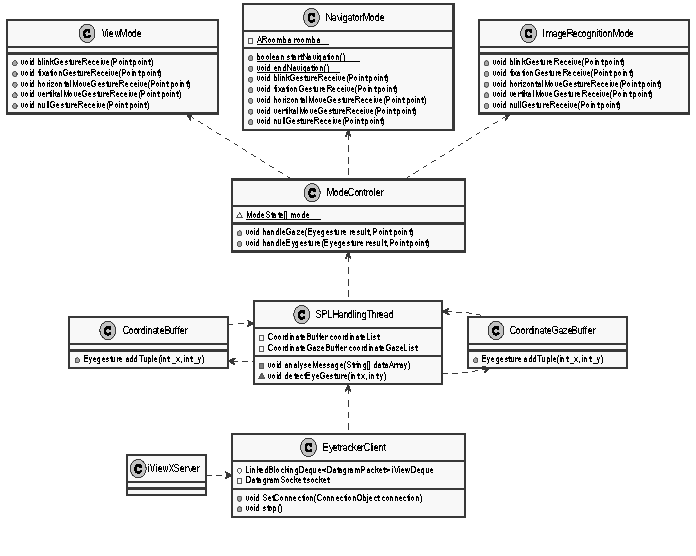
\includegraphics[width=0.9\textwidth]{bilder/uml/moduskontrolle2.pdf}
\end{center}
\caption{Darstellung der wichtigsten Klassen im Zusammenhang mit der Augengestenerkennung und der Modussteuerung.}
\label{fig:moduskontroll}
\end{figure}

\paragraph{Augengestenerkennung}
%\item[]~\hfill
\begin{enumerate}
\item Zunächst erfolgt der Empfang der UDP-Pakete vom \textit{\iV Server} durch den \textit{Eyetracking-Client}. Anschließend analysiert der \textit{SPLHandlingThread} die UDP-Nachricht und extrahiert die Befehle und Koordinaten der Kommunikation. Die Koordinaten werden der Methode \textit{detectEyegesture(int x, int y)} übergeben \cite[S.44]{Eidam2015}. 
\item \textit{detectEyegesture} übergibt die Koordinaten zum einen an die Klasse \textit{CoordinateBuffer}, zur Detektion der Augengeste (Fixation, Lidschluss, horizontal- und vertikale Augengeste) und zum anderen an den \textit{CoordinateGazeBuffer} zur Detektion der Blickgeste. Beide Klassen sind von der Klasse \textit{LinkedList<Point>} abgeleitet und beinhalten die Methode \textit{addTuple(int x, int y)}. Bei erkannter Augengeste erfolgt die Rückmeldung an den \textit{SPLHandlingThread}.
\end{enumerate}

\paragraph{Modussteuerung}
\begin{enumerate}
\setcounter{enumi}{3}
\setcounter{enumii}{1}
\item[\arabic{enumi}.] Die als Singleton angelegte Klasse \textit{ModeController} führt die Funktionalität der erhaltenen Augengeste über die Methode \textit{handleEygesture(Eyegesture result, Point point)} aus. Die Funktionalität der Blickgeste wird über die Methode \textit{handleGaze(Eyegesture result, Point point)} realisiert. \textit{ModeController} ist für die regelrechte Steuerung der unterschiedlichen Modi des Prototypen verantwortlich.
\item[\arabic{enumi}\alph{enumii}.]  Die Methode \textit{handleEygesture} führt je nach erkannter Augengeste (Fixation, Lidschluss, horizontale und vertikale Augengeste), die im Abschnitt \ref{subsection:gestKontroll} beschriebene bereitgestellte Funktionalität der einzelnen Augengesten für jeden der drei Modi aus. Im vorliegenden Prototyp wird ein Moduswechsel durch die horizontale Augengeste angeboten. Die anderen Augengesten bleiben ohne Belegung. Die Modi des Softwareprototyps implementieren alle das \textit{Interface ModeState}, das auf dem State-Entwurfsmuster basiert. 
\setcounter{enumi}{3}
\setcounter{enumii}{2}
\item [\arabic{enumi}\alph{enumii}.] Die Methode \textit{handleGaze} ist für die Steuerung des mobilen Roboters relevant und leitet die detektierten Blickkoordinaten an die Klasse \textit{NavigationsModus} weiter, die die Verbindung zum Roomba herstellt und sie beim Moduswechsel wieder abbaut. 
\end{enumerate}

\paragraph{Steuersignalerzeugung}
\begin{enumerate}
\setcounter{enumi}{3}
\item Die Herstellung einer Verbindung zum \textit{Rommba} erfolgt zunächst durch die Methode \textit{connect(ConnectionRoombaObject roombaConnection)}. Im Anschluss ist es möglich, den Roomba mit Steuerbefehlen zu bewegen, (\vgl~\acs{abb}~\ref{fig:navigationskontrolle}). 
\item In einem nächsten Schritt wird durch die Methode \textit{getCommand()} der Steuerelementeklassen  (\textit{ControlElementDiskret, ControlElementContinuous}) der erzeugte Befehl geliefert, (\vgl~\acs{abb}~\ref{fig:navigationskontrolle}). Dabei produziert jedes Steuerelement nach den in Abschnitt \ref{subsection:diskSt} \bzw \ref{subsection:kontSt} beschrieben Verfahren die Steuerbefehle. Dieses Konzept setzt das Command-Entwurfsmuster um. 
\item Die Klassen \textit{NavigatorMode} führt die Methode \textit{perform()} des aktuellen Befehls (\textit{Command}) aus. Dabei wird die Methode \textit{send(byte[] bytes)} der Klasse \textit{Roomba} realisiert und als Steuerbewegung vom mobilen Roboter umgesetzt (\vgl~\acs{abb}~\ref{fig:navigationskontrolle}). Die Frequenz der Befehlserzeugung ist dabei von der Frequenz der Blickgestendetektion abhängig. 
\end{enumerate}



\begin{figure}[ht]
\begin{center}
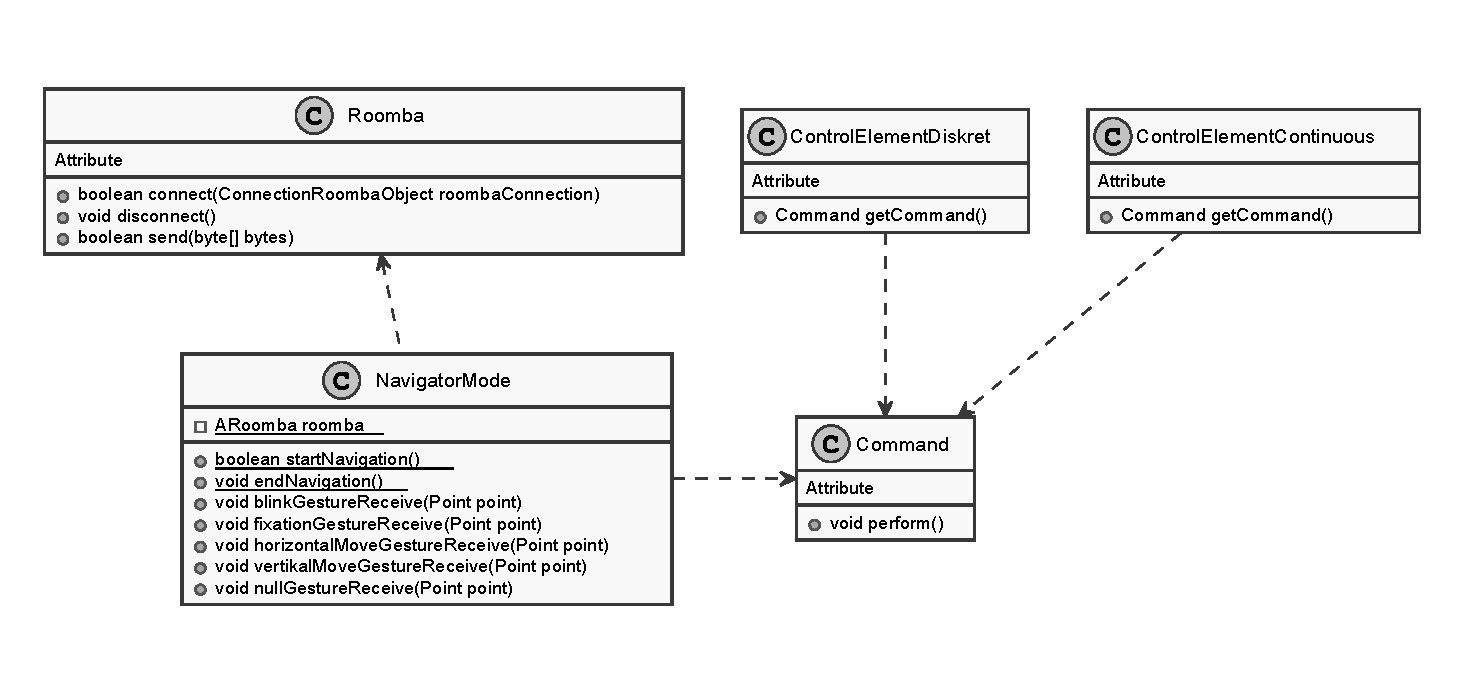
\includegraphics[width=0.9\textwidth]{bilder/uml/navigation.pdf}
\end{center}
\caption{Darstellung der wichtigsten Klassen im Zusammenhang mit der Steuersignalerzeugung.}
\label{fig:navigationskontrolle}
\end{figure}

\section{Technische Umsetzung}
\label{section:techkomp}
Folgender Abschnitt listet die Komponenten, die zur Realisierung des Softwareprototyps verwendet wurden, auf und beschreibt kurz die verwendeten externen Bibliotheken. Die bereits bei Eidam (2015) beschriebene OpenSource Software \textit{MaryTTS} wird im vorliegenden Softwareprototyp aufgrund der übernommenen Softwarearchitektur implementiert, allerdings aufgrund der nicht realisierten Objekterkennung des Prototyp, nicht verwendet \cite{Eidam2015}. 
\subsection{Basis Komponenten}
\begin{description}
\item[Programmierung:] \hfill
\begin{itemize}
\item Programmiersprache Java.
\item \acf{jdk} 1.8.0 Update 91.
\item Swing als Grafikbibliothek.
\item Externe Bibliotheken: \hfill
\begin{description}
\item JavaCV\footnote{Website und Download: \url{https://github.com/bytedeco/javacv} (letzter Aufruf: 15. Juni 2016)} (Version~1.2. [Juni 2016])
\item RoombaComm\footnote{\url{http://hackingroomba.com/code/roombacomm/} (letzter Aufruf: 25. Mai 2016)} \footnote{\url{http://roombahacking.com/software/roombacomm-0.96.zip} (letzter Aufruf: 25. Mai 2016)} (release 0.96 [September 2006]) von Tod E. Kurt und Paul Bouchier.
\end{description}  
\end{itemize}
\item[\acf{ide}:] \hfill
\begin{itemize}
\item Eclipse Java EE IDE for Web Developers (Version: Eclipse Mars.2 Release [4.5.2]).
\item Versionskontrolle durch Eclipse Git (Version: 4.4.1.201607150455-r) .
\end{itemize}
\item[Software-Zielformat]\hfill
\begin{itemize}
\item ausführbare Jar-Datei
\end{itemize}
\end{description}
\subsection{Externe Bibliotheken}
Dieser Abschnitt beschreibt kurz die beiden zusätzlich verwendeten externen Bibliotheken.
\begin{description}
\item[JavaCV (Version~1.2. [Juni 2015])] Zur Umsetzung der Videobilddarstellung des mobilen Roboters, wurde auf die frei zugängliche JavaCV-Bibliothek zurückgegriffen. JavaCV vereint wichtige Bibliotheken aus dem Bereich der Bildverarbeitung und ermöglicht die Codierung und Decodierung eines \acf{mjpeg}-Video-streams. \acs{mjpeg} ist ein Verfahren zur Codierung und Decodierung digitaler Videos, bestehend aus komprimierten Einzelbildern in JPEG-Norm\footnote{Die Bezeichnung \textit{JPEG} resultiert aus dem Namensgebenden Gremium \textit{Joint Photographic Experts Group}, welches 1992 den JPEG Standard (ISO/IEC 10918) entwickelt hat. \url{https://jpeg.org/about.html} (letzter Aufruf: 19. März 2017)}. Die verwendeten Kamera (AXIS M1034-W) stellt diesen Videostream bereit. Entscheidend für die Umsetzung der Videobilddarstellung waren die für die Bildverarbeitung notwendige Programmbibliothek \textit{OpenCV \footnote{\url{http://opencv.org/} (letzter Aufruf: 19. März 2017)}} und das Multimedia Framwork \textit{FFmpeg \footnote{\url{http://ffmpeg.org/} (letzter Aufruf: 19. März 2017)}}. 

Notwendig ist es neben den im JavaCV-Paket enthaltenen jar-Dateien, die Datei \textit{ffmpeg-3.0.2-1.2.jar} zusätzlich mit in das Projekt einzubinden.

\item[RoombaComm (release 0.96 [September 2006])] Zur Realisierung der Kommunikation des Systems mit dem verwendeten Robotersystem Roomba wurde die von Tod Kurt und Paul Bouchier bereitgestellte Java-Bibliothek zur Kommunikation und Kontrolle des Roombas für die Nutzung im Softwareprototyp modifiziert \cite{Kurt2007}.
Verwendung fanden die beiden Klasse:
\begin{itemize}
\item RoombaComm
\item RoombaCommTCPClient
\end{itemize}
\end{description}






\begin{comment}


Für die Steuerung des vorliegenden Prototypen wurde hauptsächlich die, in der Arbeit von Ediam beschriebene, Fixation als Grundlage für die benutzte Blickgeste verwendet \cite{Eidam2015}. Wie bereits im Abschnitt \ref{chapter:grundlagen} beschrieben, ist die Fixation eine Augengeste im Rahmen der Wahrnehmung. Dabei wird die Registrierung der Fixation durch den Bewegungsumfang des \acs{por} berechnet. Bewegt sich der \acs{por} des Benutzers innerhalb eines \textit{definierten Zeitraums} und innerhalb eines begrenzten Blickbereichs, wird eine Fixation erkannt \cite{Eidam2015,SMI2011}. Bei Festlegung sehr kurzer Zeiträume kann die Fixation als Blickgeste interpretiert werden. In der Arbeit von Eidam wurden für den vorliegenden Prototypen zur Steuerung des \acs{tps} die Blickgesten verwendet. Im Hinblick auf eine Nutzung des Systems, für die Möglichkeit einer Interaktion mit Objekten im Bild, ist es sinnvoll die Fixation neben einer reinen Blickgeste als Augengeste zu definieren. 


\subsubsection{Fixation}

\end{comment}
  
  % Kapitel 5
 % kapitel5.tex
\externaldocument{C_anhang.tex}
\chapter{Evaluation}
\label{chapter:evaluation}

\section{Versuchsaufbau}
\label{section:versuchsaufbau}
Im Folgenden werden der Versuchsaufbau und die Versuchsdurchführung beschrieben.

\subsection{Komponenten}

\paragraph{Eyetracking}
Die Komponenten des Eyetracking werden in \acs{abb}~\ref{fig:komponenten} gezeigt. Der stimuluspräsentierende Bildschirm ist über einen eigenen PC mit der Workstation verbunden. Die Workstation ist mit der \acs{et} konnektiert und führt die \iV Software aus. 

\begin{figure}[ht]
\begin{center}
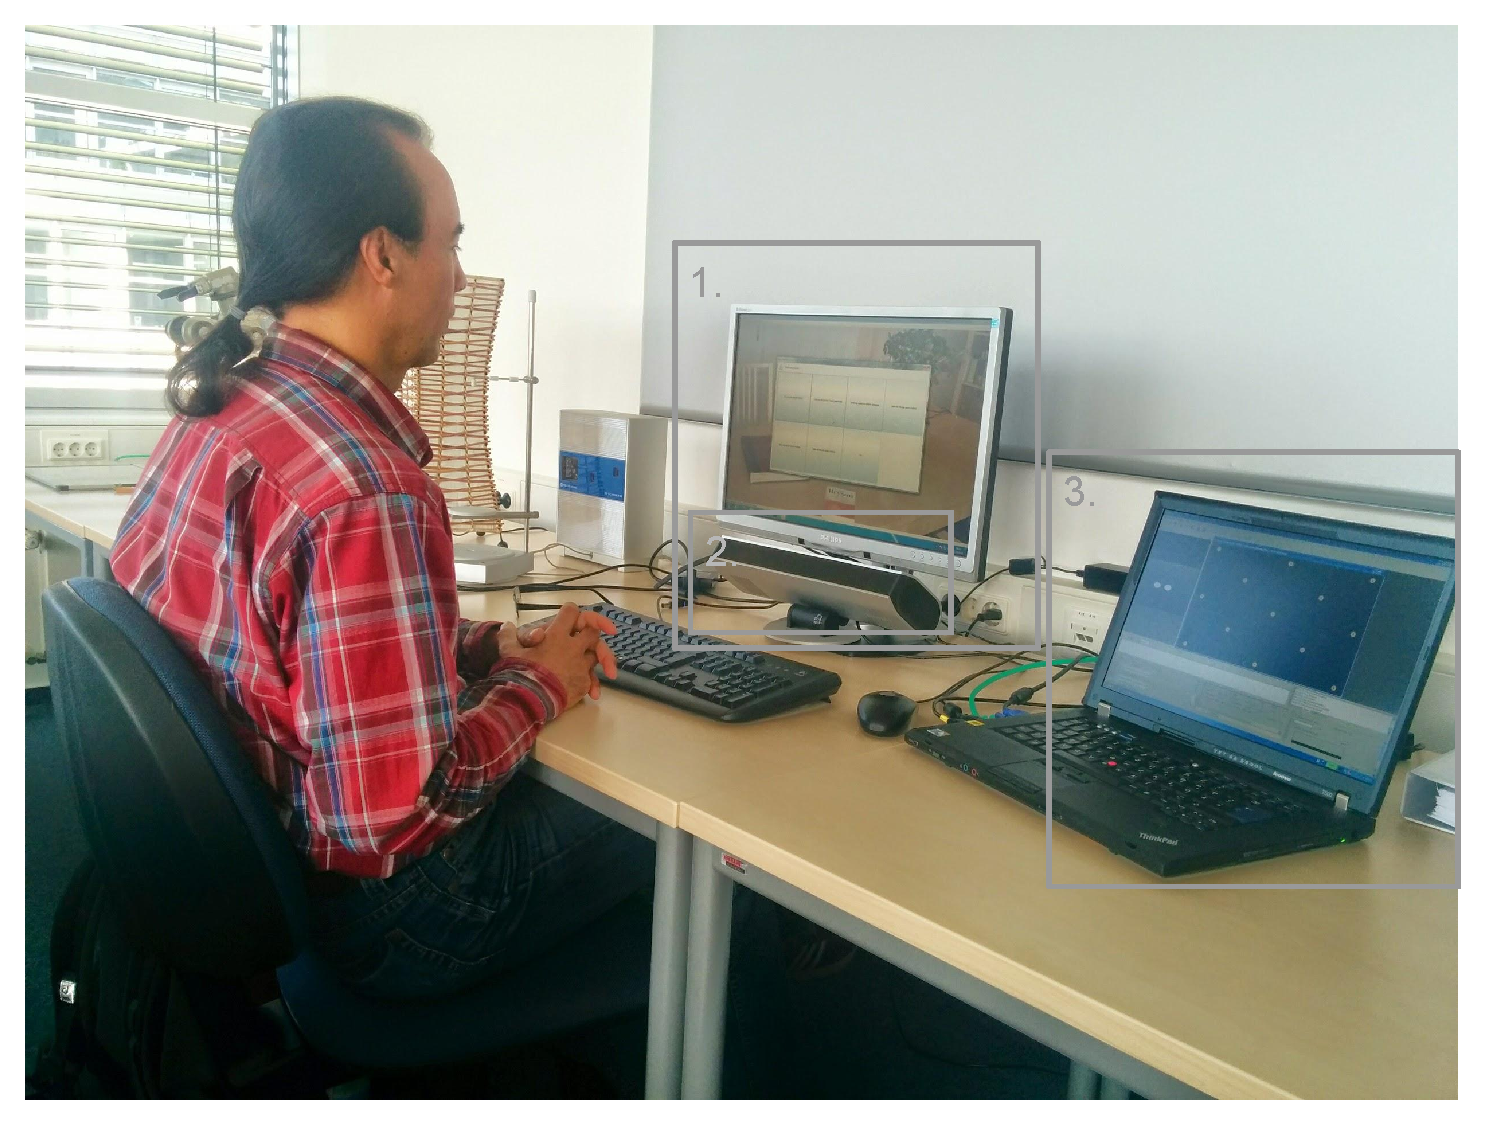
\includegraphics[width=0.7\textwidth]{bilder/evaluation/anordung.pdf}\hfill
\end{center}
\caption{Komponenten des Eyetracking. Die Darstellung zeigt eine Testperson während der Verwendung des Softwareprototyp von Eidam (2015). Dieser Aufbau wurde für die vorliegende Arbeit übernommen.  (1.)~\acs{spb}, (2.)~\acs{et}, (3.)~\iV ~\acs{wo}. (Bild:~modifiziert aus \cite[S.51]{Eidam2015})}
\label{fig:komponenten}
\end{figure}

Bei der Versuchsdurchführung ist auf eine adäquate Sitzpositionierung der Testperson im Verhältnis zum Bildschirm zu achten. Die Augen der Testperson sollten von einer tiefer angeordneten Position der RED observiert werden, \vgl~\acs{abb}~\ref{fig:empfehlung}. Grundsätzlich soll ein freies Sichtfeld gewährleistet sein.

\paragraph{\acf{tps}}
Der als Telepräsenzsystem modifizierte Roomba 620 wird in \acs{abb} \ref{fig:subroomba} dargestellt. Zu erkennen ist die zentrisch angeordnete Kamera der Firma Axis (AXIS M1034-W) und der Access-Point, der an der seriellen Schnittstelle des Roombas angeschlossen ist. Der Access-Point dient unter Zuhilfenahme von \enquote{socat}-Prozessen dazu, die Netzwerkkommunikation zu ermöglichen. \enquote{Socat} ist ein Tool, um Datenströme unter Linux/Unix-Systemen verbinden zu können. Für die vorliegende Arbeite wurde \enquote{socat} so konfiguriert, dass es an einem Netzwerk-Socket (einem TCP-Port) lauscht und die Daten der TCP-Pakete an den seriellen Port weiter leitet. Im Gegenzug werden die Daten aus der seriellen Schnittstelle an die zuletzt geöffnete TCP-Verbindung zurückgeliefert. %Auf die Nutzung dieser zweiten genannten Verbindungsrichtung wurde im Rahmen der vorliegende Arbeit verzichtet.
 
\begin{figure}[ht]
\begin{minipage}[b]{\linewidth} 
      \centering 
  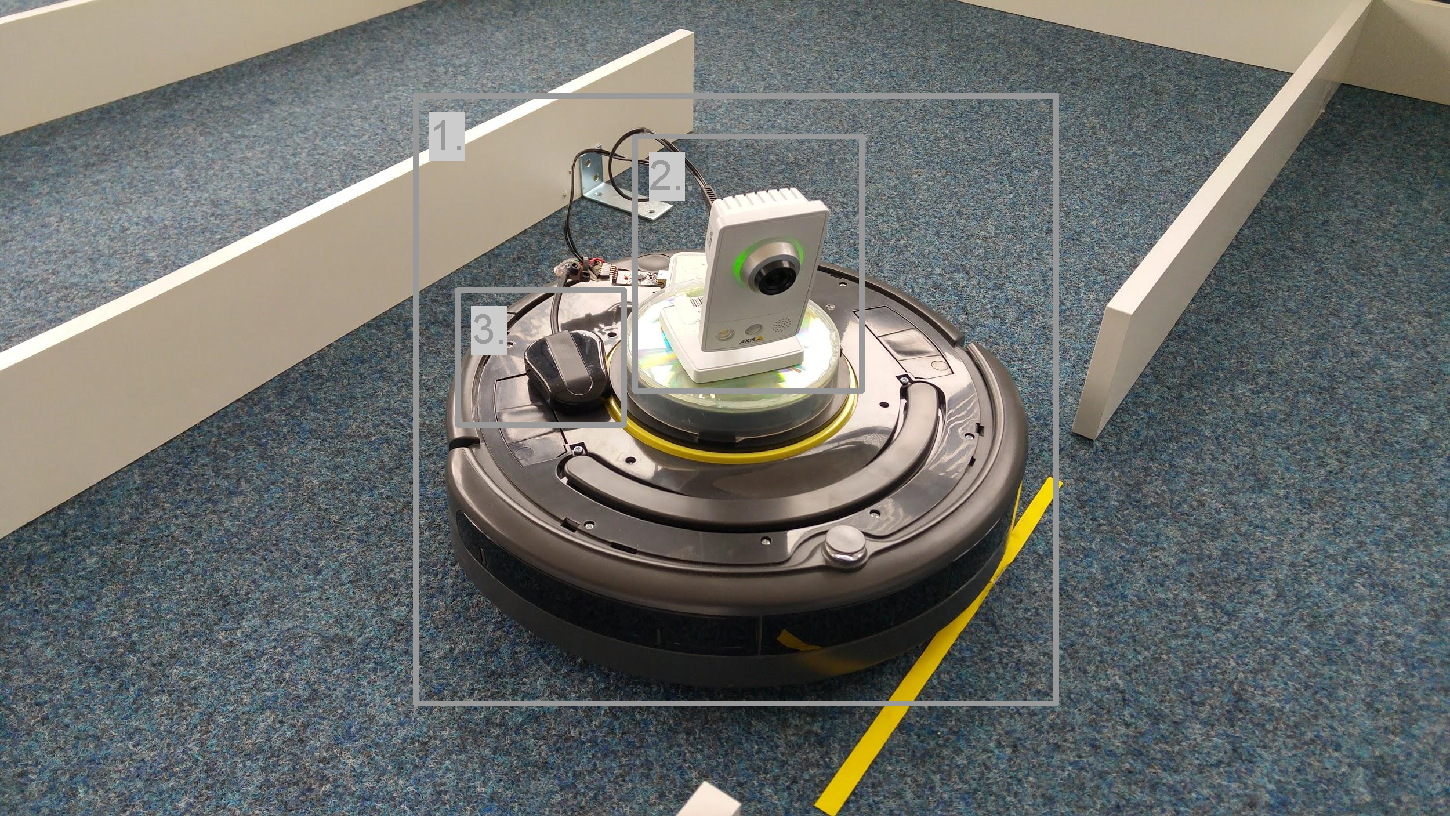
\includegraphics[width=0.7\linewidth]{bilder/evaluation/roomba.pdf}
  \label{fig:subroomba} 
   \end{minipage}%
\caption{Verwendetes \acl{tps} während der Parcoursdurchquerung. (1.)~Roomba 620 modifiziert als \acl{tps}, (2.)~mittig angeordnete Videokamera, (3.)~Access-Point zur Netzwerkkommunikation.}
\label{fig:subroomba}
\end{figure}


\subsection{Testpersonen}
Für die Durchführung der Parcoursaufgabe und der Evaluation des Fragebogens stellten sich insgesamt fünf körperlich unbeeinträchtigte Testpersonen zu Verfügung. Vier Personen aus dem Lehrgebiet der Mensch-Computer-Interaktion des Fachbereichs Mathematik und Informatik der FernUniversität Hagen nahmen freiwillig daran teil. Ferner beteiligte sich der Verfasser dieser Arbeit ebenfalls an Evaluation und Parcoursaufgabe. In Bezug auf die Nutzung von Eyetracking-Systemen unterschieden sich die Teilnehmer in ihren Vorerfahrung, die aber nicht weiter differenziert oder unterschieden wurde. Jede Testperson bekam vor der Kalibrierung des Eyetracking-Systems eine kurze Einführung in die grundlegenden Funktionsweisen der beiden Steuerungsmodi und war im Anschluss angehalten, nach eigenem Ermessen die Parcoursbewältigungsaufgabe durchzuführen.

\subsection{Testparcours}
Der eigentliche Testparcours befindet sich innerhalb eines Bereichs der Größe 200 cm x 200 cm. Hierbei wird der Bereich durch einen 80 cm x 80 cm großen Ladestationsbereich erweitert. Der Zugang zum eigentlichen Parcours ist durch eine Eingangsbarriere der Größe von 40 cm festgelegt. Innerhalb dieses Abschnittes ist eine Art \enquote{Kreisbahn} durch eine 50 cm breite \enquote{Strecke} eingerichtet, siehe \acs{abb}~\ref{fig:aufbau}.

\begin{figure}[ht]
\begin{center}
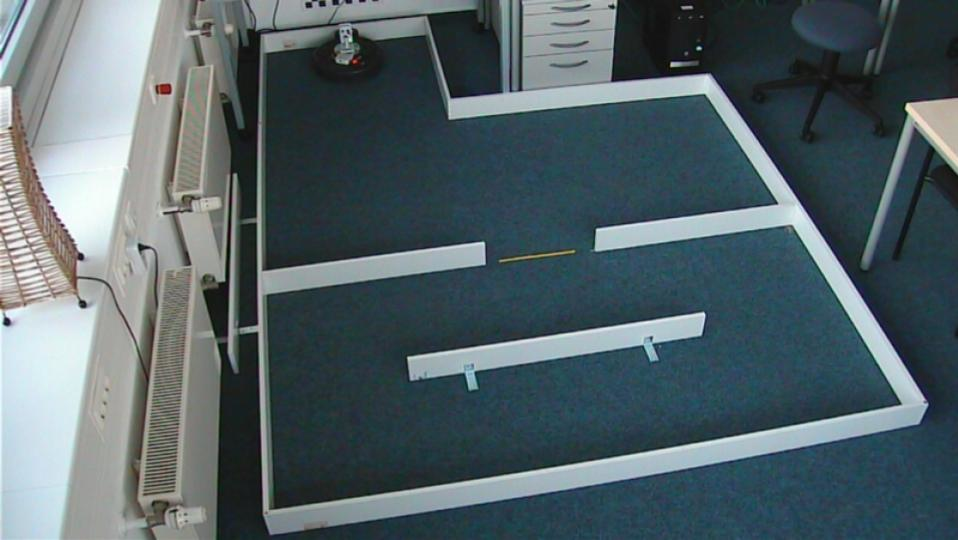
\includegraphics[width=0.7\textwidth]{bilder/evaluation/TopView.png}\hfill
%\includegraphics[scale=0.2]{bilder/evaluation/Parcour.png}
\end{center}
\caption{Parcours-Versuchsaufbau mit einer Ansicht von oben. Zu erkennen ist der eigentliche Testparcours. Start und Stopp sind anhand der gelben Markierung in der Eingangsbarriere auszumachen.}
\label{fig:aufbau}
\end{figure}


\section{Versuchsdurchführung}
\label{section:versuchsdurchführung}
Die folgenden Systemeinstellungen wurden von allen beteiligten Testpersonen verwendet. Die Einstellungen kamen für beide Steuermethoden zum Einsatz. Prinzipiell konnten die Einstellungen frei gewählt werden. Alle Benutzer entschieden sich jedoch für die Standardeinstellung:

\begin{itemize}
 \item[-] 1000 ms Fixierungsdauer,
 \item[-] 250 ms minimale Lidschlussdauer und 500 ms maximale Lidschlussdauer,
 \item[-] 200 px maximale Dispersion,
 \item[-] 200 px maximale Auslenkung in Bezug auf die horizontale und vertikale Augengestenerkennung.
\end{itemize}

Zur Messung der Steuerung wurde ein Parcoursaufgabe konzipiert, wobei die zurückgelegte Zeit als quantitatives Messkriterium herangezogen wurde. Ziel dieser Anordnung war es, die Aufgabe in einer möglichst kurzen Zeit zu bewältigen. Die Vermeidung von Kollisionen war beabsichtigt, jedoch kein Abbruchkriterium. Die Aufgabe galt als erfolgreich beendet, wenn der Parcours ausgehend von der Startmarkierung einmal umfahren und anschließend die Markierung überquert wurde. Die Richtung der Durchführung blieb den Testpersonen überlassen und wurde nicht unterschieden.

Nach Abschluss der Parcoursaufgabe wurde zur Klärung der Gebrauchstauglichkeit (Usability) des Prototyps ein eigens konzipierter Fragebogen mit den in Kapitel~\ref{sect:testmerkmale} Testmerkmalen beantwortet, \vgl Anhang~\ref{chapter:ergabb}. 


 
  % Kapitel 6
 % kapitel6.tex
\externaldocument{02_grundlagen.tex}
\chapter{Ergebnisse und Diskussion}
\label{chapter:ergebnisse}

\section{Versuchsergebnisse}
\label{section:versuchsergebnisse}

Im folgenden Kapitel werden zunächst die Ergebnisse der Evaluation dargestellt und im Anschluss folgt die Diskussion der gewonnenen Ergebnisse. 

\subsection{Parcoursdurchführung}
Mittels der Zeitmessung während der Parcoursbewältigungsaufgabe sollte die Machbarkeit der bereitgestellten Steuerungsmethoden (diskret und kontinuierlich) demonstriert und abgeschätzt werden. 
\acs{tab} \ref{tab:parcourzeit} und die \acs{abb} \ref{fig:parcourzeit} zeigen die ermittelten Durchführungszeiten der Testpersonen der Testparcoursaufgabe.

\begin{figure}[ht]
\begin{center}
\fbox{\includegraphics[width=0.7\textwidth]{bilder/ergebnisse/parcours680x400.pdf}}
\end{center}
\caption{Zeit der Parcoursbewältigung der fünf Testpersonen (\enquote{A},\enquote{B},\enquote{C},\enquote{D},\enquote{E}) in Abhängigkeit der Steuerungsmethode (Zeit in Sekunden).}
\label{fig:parcourzeit}
\end{figure}


\begin{table}[h]
\centering
\begin{tabular}{crrrrr}
  \hline
 & A & B & C & D & E \\ 
  \hline
diskret & 120 &  63 & 120 & 105 &  96 \\ 
  kontinuierlich &  96 &  36 & 180 & 166 &  92 \\ 
   \hline
\end{tabular}
\caption{Zeit der Parcoursbewältigung der fünf Testpersonen (\enquote{A},\enquote{B},\enquote{C},\enquote{D},\enquote{E}) in Abhängigkeit der Steuerungsmethode (\enquote{diskret}, \enquote{kontinuierlich}) (Angaben in Sekunden).} 
\label{tab:parcourzeit}
\end{table} 

Wie in \acs{abb}~\ref{fig:parcourzeit} zu erkennen ist, konnte jede der Testpersonen die gestellte Parcoursaufgabe mittels der beschriebenen Steuermethoden bewältigen. Testperson \enquote{B} zeigte im Vergleich für beide Steuermethoden die geringste Durchführungszeit und Testperson \enquote{C} benötigte für die kontinuierliche Steuermethode am längsten. Die minimale Durchführungszeit konnte mit der kontinuierlichen Methode erzielt werden (36 Sekunden). Die maximale Durchführungszeit wurde ebenfalls mit der kontinuierlichen Steuerungsmethode erzielt (180 Sekunden), \vgl~\acs{tab}~\ref{tab:parcourstat}. Die durchschnittliche Durchführungszeit lag bei der diskreten Steuermethode bei 100.8 Sekunden und bei der kontinuierlichen bei 114 Sekunden, \vgl~\acs{tab}~\ref{tab:parcourstat}. Bei drei der fünf Testpersonen war die Durchführungszeit der kontinuierlichen Steuermethode im Vergleich zur diskreten Steuerungsmethode schneller. 

\begin{table}[h]
\centering
\begin{tabular}{lcc}
  \hline
 &    diskret & kontinuierlich \\ 
  \hline
Min.   :&  63   & 36   \\ 
 Median : & 105  & 96   \\ 
 Mean   : & 100.8   & 114   \\  
 Max.   : & 120  &    180   \\ 
   \hline
\end{tabular}
\caption{Tabelle des Minimum (Min), Maximum (Max), Median (Median), arithmetischer Durchschnitt (Mean) in Abhängigkeit der Steuermethode.} 
\label{tab:parcourstat}
\end{table}

\subsection{Unerwünschte Ausführungen}
Bei der Benutzung des Prototyps kam es zu unbeabsichtigten Ausführungen. \acl{abb}~\ref{fig:ausführungen} zeigt deren Häufungen im Verhältnis zu den möglichen Aktionen.
\begin{figure}[ht]
\begin{minipage}[t]{\linewidth} 
\centering
\fbox{\includegraphics[width=0.7\textwidth]{bilder/ergebnisse/ausfuehrungen880x4402.pdf}}
\caption{Unerwünschte Ausführungen während des gesamten Durchführungszeitraums.}
\label{fig:ausführungen}
  \end{minipage}% 
\end{figure}

Die Auswertung der Mehrfachantworten zeigt, dass keine der Personen unerwünschte Ausführungen bei der horizontalen- und vertikalen Augengeste oder den Steuerkommandos hatte. Dies gilt sowohl für die diskrete, als auch für die kontinuierliche Steuermethode. Bei vier der fünf Benutzer war der Lidschluss während der kontinuierlichen Steuermethode in Bezug auf unerwünschte Ausführungen die problematischste Augengeste. Während der Ausführung der diskreten Steuermethode kam es zu keinen unerwünschten Ausführungen beim Lidschluss. Bei der Ausführung des kontinuierlichen Steuermodus traten bei zwei Personen während des Stoppmechanismus unerwünschte Ausführungen auf. Die Nutzung des kontinuierlichen Steuermodus verlief während des Stoppmechanismus bei allen Testpersonen störungsfrei. Die Blickbewegung führte sowohl während der Nutzung des kontinuierlichen, als auch des diskreten Steuermodells zu unerwünschten Ausführungen bei jeweils zwei Testpersonen. 
Die Möglichkeit einer zusätzlichen Angabe durch die Option \enquote{Sonstiges} wurde von zwei Personen genutzt.
Eine Testperson gab sowohl für die diskrete, als auch für die kontinuierliche Steuermethode an, dass unerwünschte Ausführungen während der Kopfbewegung auftraten. Eine Testperson hatte während der Nutzung der kontinuierlichen Steuermethode Probleme, weil das System \enquote{gelegentlich nicht mehr auf Augengesten} reagierte. 


\subsection{Ermüdung}
Mittels der vierstufigen Ratingskala wurde nach der Ausführung der Parcoursbewältigungsaufgabe abgeschätzt, als wie ermüdend die beiden angebotenen Steuermethoden empfunden wurden. \acl{abb}~\ref{fig:ermüdung} veranschaulicht die Angaben grafisch.
\begin{figure}[ht]
\begin{minipage}[b]{\linewidth} 
      \centering 
\fbox{\includegraphics[width=0.7\textwidth]{bilder/ergebnisse/ermuedung680x400.pdf}}
\caption{Diagramm zur Bewertung der Ermüdung}
\label{fig:ermüdung}
   \end{minipage}% 
\end{figure}
\begin{comment}
\begin{figure}[ht]
   \begin{minipage}[b]{\linewidth} 
      \centering 
     %\includegraphics[scale=1]{bilder/grundlagen/als.pdf}
     % \includegraphics[width=1\textwidth]{bilder/grundlagen/1als.pdf}
     \fbox {\includegraphics[width=\textwidth, height=100mm]{bilder/grundlagen/Ermu_dung.pdf}}
   \end{minipage}% 
\caption{Diagramm zur Bewertung der Ermüdung}
\label{fig:ermüdung}
\end{figure} 
\end{comment}


Die \acl{abb}~\ref{fig:ermüdung} veranschaulicht, dass alle fünf Testpersonen die Steuerung mittels diskreter Steuermethode als \enquote{wenig ermüdend} eingestuft haben. Die kontinuierliche Steuermethode wurde lediglich von zwei Testpersonen als \enquote{wenig ermüdend} eingeschätzt, während drei weitere Personen sie als \enquote{ermüdend} empfanden. 

\subsection{Handling}
Neben den unerwarteten Ausführungen und der Ermüdung, wurde als drittes Merkmal mithilfe der vierstufigen Ratingskala abgeschätzt, wie einfach das Handling der beiden Steuerungsmethoden empfunden wurde. \acl{abb}~\ref{fig:handling} zeigt die Angaben der Testpersonen grafisch.
\begin{figure}[ht]
\begin{minipage}[t]{\linewidth} 
      \centering 
\fbox{\includegraphics[width=0.7\textwidth]{bilder/ergebnisse/handling680x400.pdf}}
\caption{Diagramm zur Bewertung des Handlings.}
\label{fig:handling}
   \end{minipage}% 
\end{figure}

Wie in \acs{abb}~\ref{fig:handling} ersichtlich, empfanden vier der fünf Testpersonen die Steuerung mittels der diskreten Steuermethode als \enquote{einfach}, nur eine Person stufte sie als \enquote{schwer} ein. Die kontinuierliche Steuermethode wurde von drei Testpersonen als \enquote{einfach} eingeschätzt, zwei Personen empfanden sie als \enquote{schwer}. Keine der Testpersonen empfand das Handling der Steuerung als \enquote{sehr einfach} oder \enquote{sehr schwer}. Im Vergleich zur kontinuierlichen Steuermethode wurde die diskrete Steuermethode hierbei tendenziell einfacher wahrgenommen und evaluiert.

\subsection{Panikschalter}
Als weiteres Merkmal wurde mittels der \og vierstufigen Ratingskala abgeschätzt, wie einfach das Handling des Panikschalters der beiden Steuerungsmethoden empfunden wurde. \acl{abb}~\ref{fig:panikschalter} stellt die Angaben der Testpersonen grafisch dar. Hierbei machte eine der Testpersonen keine Angaben, weshalb nur bei (n=4) der Testpersonen eine Einschätzung möglich war. 
\begin{figure}[hbt]
\centering
\fbox{\includegraphics[width=0.7\textwidth]{bilder/ergebnisse/panikschalter680x400.pdf}}
\caption{Diagramm zur Bewertung des Panikschalters.}
\label{fig:panikschalter}
\end{figure}

Die \acl{abb}~\ref{fig:panikschalter} zeigt, dass zwei der vier Testpersonen das Handling des Panikschalters mittels der diskreten Steuermethode als \enquote{sehr einfach} und zwei Testpersonen dies als \enquote{einfach} einstuften. Im Fall der kontinuierlichen Steuermethode wurde von zwei Testpersonen die Einschätzung \bzgl des Panikschalters als \enquote{einfach} und von zwei weiteren Personen als \enquote{schwer} eingestuft. Keine der Testpersonen empfand das Handling des Panikschalters als \enquote{sehr schwer}. Der Panikschalter wurde während der Nutzung der diskreten Steuermethode,- (im Vergleich zur kontinuierlichen Steuermethode) als einfach wahrgenommen und evaluiert.

\subsection{Erweiterte Steuerungsoptionen}
Erweiterte Steuerungsoptionen wurden mittels Mehrfachantwort durch die Benutzer erfragt.
Die Auswertung zeigt, dass sich alle fünf Testpersonen eine Erweiterung der Steuerung um eine Kollisionsvermeidung wünschten. Keiner der fünf Beteiligten wünschte sich eine Augmentation der Steuerung um die Möglichkeit einer \enquote{Fahre an Ort (GOTO)}-Option oder einer \enquote{Folge einer Person (Follow)}-Option. Auch die zusätzliche Option einer Routenplanung wurde von keiner der Testpersonen gewünscht. 

Die Möglichkeit einer zusätzlichen Angabe durch die Option \enquote{Sonstiges} wurde von drei Personen genutzt.
Eine Testperson hielt die Steuerung mittels eines \enquote{Skalierungsfaktors} im Rahmen der kontinuierlichen Steuerung für wünschenswert. Eine weitere Testperson wünschte sich die Möglichkeit, die Kameraposition zu verändern, und eine Kamera, die den mobilen Roboter aus der Sicht einer dritten Person zeigt. Die dritte Testperson erachtete eine Anzeige zur Visualisierung des Abstandes zu Objekten in der unmittelbaren Umgebung des mobilen Roboters als wünschenswert.

\subsection{Gesamtbewertung}
Als Gesamtbeurteilung vergaben die Testpersonen Schulnoten auf einer Skala, die in \acs{abb}~\ref{fig:gesamtnoten} dargestellt ist.  
\begin{figure}[htb]
\begin{center}
\fbox{\includegraphics[width=0.7\textwidth]{bilder/ergebnisse/Gesamtbewertung.png}}
\end{center}
\caption{Gesamtbewertung in Schulnoten.}
\label{fig:gesamtnoten}
\end{figure}

Vier der fünf Testpersonen bewerteten die diskrete Steuerungsmethode mit \enquote{gut = 2}, einer der Benutzer mit \enquote{befriedigend = 3}. Die kontinuierliche Steuerungsmethode wurde von zwei der fünf Testpersonen mit \enquote{gut = 2} und von zwei weiteren mit \enquote{befriedigend = 3} bewertet. Die fünfte Testperson vergab hierfür die Note \enquote{ausreichend = 4}. Für beide Testmethoden wurden weder die Noten \enquote{sehr gut = 1}, noch die Bewertungen \enquote{mangelhaft = 5} oder \enquote{ungenügend = 6} vergebenen, siehe \acs{abb}~\ref{fig:gesamtnoten}.

\section{Diskussion}
\label{section:Diskusion}
Mobile~\aclp{tps} mittels definierter Augengesten zu steuern, ist -wie im Abschnitt~\ref{chapter:grundlagen} gezeigt wurde- eine anspruchsvolle Aufgabe. Das Ziel der vorliegenden Arbeit ist es, zwei unterschiedliche Lösungsstrategien für die Steuerung eines Telepräsenzrobotersystems in einem Softwareprototypen zu realisieren und diese \bzgl der Machbarkeit, der Präzision, der Handhabung, der Ermüdung und in Bezug auf die Nutzung eines Panikschalter zu vergleichen.
Es folgt die Diskussion der in Kapitel~\ref{section:versuchsergebnisse} beschriebenen Ergebnisse. Zunächst werden die beiden Steuerungsmethoden diskutiert und im Anschluss folgt die Diskussion der Testparameter und der Testpersonen.


\subsection{Diskussion der Steuerungsmodelle}
%Mittels der Zeitmessung während der Parcourbewältigungsaufgabe konnte die Machbarkeit der bereitgestellten Steuerungsmethoden (diskret, kontinuierlich) demonstriert werden. Die Evaluationsergebnisse zeigen, dass die Umsetzung einer Steuerung eines mobilen Roboters mithilfe eines Eyetrackers erfolgreich umgesetzt werden konnte. 

Die \og Evaluationsergebnisse demonstrieren, dass alle beteiligten Testpersonen die Parcoursaufgabe bewältigen konnten. Damit ist es grundsätzlich möglich, ein mobiles Robotersystem durch einen \enquote{einfachen}~Parcours nur mittels der Augen zielgerichtet zu manövrieren. Die bereitgestellten Steuerungsmethoden (diskret, kontinuierlich) wurden hierbei so konzipiert, dass eine \enquote{einfache} Basissteuerung durch das \textit{diskrete}~Steuermodell und eine \enquote{anspruchsvollere}~Steuerungsform durch die \textit{kontinuierliche} Steuermethode miteinander verglichen werden konnten. 
Wie die Gesamtbewertung zeigt, wurde die diskrete Steuermethode seitens der Testpersonen im Vergleich zur kontinuierlichen Steuerung tendenziell besser bewertet. Hierfür sprechen mehrere Gründe: Wie in \acs{abb}~\ref{fig:ausführungen} gezeigt, sind zum einen die unerwünschten Ausführungen während der Nutzung der diskreten Steuermethode insgesamt seltener aufgetreten. Dies kann seitens der Testpersonen positiv aufgefasst worden sein. Ferner kann das Fehlen der unerwünschten Ausführungen zu einem einfacheren Ablauf während der Steuerung geführt und die Bewertung beeinflusst haben. Der Faktor der \textit{Ermüdung} spielt für das Empfinden und damit die Bewertung ebenfalls eine wichtige Rolle. Die diskrete Steuerungsmethode wurde im Vergleich zur kontinuierlichen  als \enquote{weniger ermüdend} wahrgenommen. Auch in der Handhabung (Handling) wurde die diskrete Steuermethode tendenziell als einfacher empfunden. Darüber hinaus ist in Bezug auf die Nutzbarkeit das Stoppen des mobilen Roboters wichtig. Ein fehlendes Ansprechen bei einem Stoppkommando kann in kritischen Situationen unter Umständen zu schwerwiegenden Komplikationen führen. Daher ist der Stoppmechanismus für die Steuerung entscheidend.

Bezüglich der gemessenen Durchführungszeiten variierten die Ergebnisse teilweise deutlich zwischen den verschiedenen Testpersonen, siehe \acs{abb}~\ref{fig:parcourzeit}. Ein Hauptgrund dafür lag vermutlich in einem unterschiedlichen Erfahrungsniveau der Testpersonen in Bezug auf die Nutzung von Eyetracking-Systemen. Es zeigte sich jedoch, dass selbst gänzlich unerfahrenen Testpersonen der Zugang zur Nutzung eines Eyetracking-Systems und somit zur Steuerung des mobilen Roboters nach kurzer Zeit möglich war. Personen mit Bewegungseinschränkungen könnten von diesem Aspekt der relativ steilen Lernkurve profitieren. Alternative Mensch-Computer-Schnittstellen, wie beispielsweise abgeleitete Hirnstrommessungen mittels Elektroenzephalogramm (EEG), die zur Steuerung benutzt werden können, zeigen hier eine längere Eingewöhnungszeit, \vgl~\cite{Tonin2011}. Ferner sind diese Verfahren nach individueller Anpassung nicht problemlos auf andere Anwender übertragbar und müssen kalibriert werden. Die notwendige Kalibrierung der Eyetracking-Systeme ist bei vorhandener Augenmotorik relativ leicht umsetzbar. 
%Insgesamt ist es im Hinblick auf die \og Ergebnisse als ein gutes Ergebnisse zu werten, dass alle Testpersonen 

\subsection{Diskussion der Testmerkmale}
Die Arbeitsfragen bezüglich der Machbarkeit, der Präzision, des Handlings und die Fragen, wie ermüdend diese Art der Steuerung ist und ob Unterschiede zwischen einer diskreten und kontinuierlichen Steuerungsform vorhanden sind, wurden mittels eines eigens entworfenen Fragebogens beantwortet. Hierbei wurde versucht, die Machbarkeit und die Präzision durch die Quantifizierung der Durchführungszeit einer Parcoursaufgabe zu messen. Damit sollte eine einfache Vergleichbarkeit der beiden Steuerungsmethoden erreicht werden. Ferner wurde eine qualitative Bewertung des Handlings, der Ermüdung und des Panikschalters untersucht. Um die Motivation der Teilnehmer zu erhöhen, wurde der Fragebogen \bzgl der Ausfüllzeit kurz gehalten. 

\subsection{Diskussion der Testpersonen}
Bei der Durchführung der Evaluation und der Benutzung des Prototyps wurden fünf gesunde Testpersonen befragt und \bzgl der Parcoursaufgabe getestet. Die Vorerfahrung der Benutzer wurde nicht differenziert unterschieden. Allerdings waren vier der Testpersonen aus dem Lehrgebiet der Mathematik und Informatik und damit der Nutzung von technischen Hilfsmitteln zumindest nicht abgeneigt. Damit muss zumindest ein gewisser Vorerfahrungsfaktor angenommen werden, der einen Einfluss auf die allgemeine Bewertung haben kann. Jedoch ist durch die Vorerfahrung der beteiligten Personen sicherlich eine kritischere Auseinandersetzung möglich und damit eine differenziertere Bewertung. Im Hinblick auf die geplante zukünftige Nutzergruppe ist eine Anzahl von lediglich fünf Testpersonen wenig aussagekräftig. Als Folgeschritt erscheint es sinnvoll, den Prototyp durch eine größere Anzahl von Personen zu testen.

\subsubsection{Kritische Anmerkungen}
Während der Ausführung der Parcoursbewältigungsaufgabe war die zentrische Positionierung der Kamera auf dem mobilen Roboter ein kritischer Punkt. Hierdurch war das Blickfeld derart eingeschränkt, dass es zu Fehleinschätzungen der Abstände beim Fahren kam. während der Fahrt kam Dadurch wurden \enquote{Hindernisse} innerhalb des Parcours \enquote{übersehen}, was zu Kollisionen führte und weshalb Versuche abgebrochen wurden. Es ist jedoch zu erwähnen, dass dies nicht der fehlenden Präzision der Steuerung zuzuschreiben war, sondern einzig der Blickfelddarstellung. In diesem Maße muss aufgrund dieser Tatsache jedoch angemerkt werden, dass für die effiziente Steuerung so wichtige situation~awareness~(SA) aufgrund der unvollständigen visuellen Rückmeldung nicht adäquat gegeben war. Wie entscheidend die \acs{sa} für eine effiziente Steuerung ist, zeigen die Arbeiten von~\cite{Yanco2004-2}.   

Die Tatsache, dass alle Personen eine Kollisionsvermeidung als nützliche Ergänzung erachtet haben, deutet darauf hin, dass der kognitive Aufwand zur Steuerung besonders auf der Vermeidung von Kollisionen lag. Deutlich sinnvoller erscheint es, die Nutzung der kognitiven Ressourcen (Aufmerksamkeit, Konzentrationsfähigkeit, Merkfähigkeit) für die Interaktion mit der unmittelbaren Umgebung zu verwenden. Gerade im Hinblick auf die geplante Anwendergruppe scheint dies daher, eine zielführende Bedingung zu sein. Die Arbeit von Baldo et al. bestätigen den Effekt einer unterstützenden Kollisionsvermeidung (Shared~Control) in Bezug auf eine erleichterte Steuerung~\cite{Baldo2015}.

  % Kapitel 7
  % kapitel7.tex
\chapter{Zusammenfassung und Ausblick}
\label{chapter:zusammenfassung}

Ziel dieser Abschlussarbeit war es, für ein einfaches \acl{tps} zwei unterschiedliche blick- und augengestenbasierte Steuerungsmethoden in Form eines Softwareprototyps zu realisieren. Hierfür wurde ein mobiler Staubsaugerroboter durch die Augmentierung um eine Kamera zu einem einfachen \acl{tps} umfunktioniert. Mittels der visuellen Rückmeldung des Systems,- war es einer Gruppe von fünf gesunden freiwilligen Testteilnehmern möglich, eine entworfene Parcoursaufgabe durch Teleoperation\footnote{Im Sinne von \enquote{Fernsteuerung}} des \acs{tps}, einzig auf Blick- und Augengesten basierend, zu bewältigen. 

Zur Detektion der Blick- und Augengesten wurde ein stationäres videobasiertes Eye\-track\-ing-System verwendet, das mittels des Dark-Pupil-Verfahrens den \acl{por} des Benutzers berechnet und damit die Augengesten erkennt. Dabei konnte durch insgesamt vier verwendeten Augengesten (Fixation, Blickgeste, Lidschluss, vertikaler Augenbewegung) die Interaktion mit der Benutzerschnittstelle des Systems realisiert werden. 

Die anschließende Befragung der Testteilnehmer mittels eines selbst entworfenen Fragebogens zeigte, dass eine Steuerung nur auf Blick- und Augengesten aufbauend,- von den Testpersonen größtenteils gut aufgenommen und akzeptiert wurde. Im Rahmen der differenzierten Befragung ließ sich eine leichte Präferenz hin zu einer der beiden Steuerungsmethoden erkennen. Diese präferierte \textit{diskrete}~Steuermethode stellt im Grunde vier Richtungspfeiltasten einer Tastatur im Blickfeld der Testperson dar und ermöglichte so die einfache Interaktion mit dieser Steuerkomponente. Die \textit{kontinuierliche}~Steuerungsmethode (als zweite Steuermethode), bei der die Augen als eine Art Steuerhebel fungierten, wurde ebenfalls als adäquate Möglichkeit einer Blick- und Augengestensteuerung erachtet. In Bezug auf das Handling, die Ermüdung, die Umsetzung eines unmittelbaren Stoppmechanismus und allgemein im Hinblick auf die Gesamtbewertung wurde diese Steuermethode jedoch von der Mehrzahl der Testpersonen nicht favorisiert. Die Befragung zeigte außerdem, dass die Implementierung einer Kollisionsvermeidung für die Teleoperation eine sinnvolle Erweiterung bieten kann. 

Obwohl die vorliegende Arbeit die Methodik der blick- und augenbasierten Steuerung nur mit einer kleinen Zahl von motorisch unbeeinträchtigten Personen getestet hat, liefert diese Arbeit Hinweise darauf, dass eine Steuerung eines mobilen Roboters mithilfe eines Eyetracking-Systems auch durch Personen mit Bewegungseinschränkungen bei erhaltener Okulomotorik möglich ist.

Im Hinblick auf eine zukünftige Nutzung einer Kombination aus Eyetracking-System und mobilen \acl{tps} stellt die sichere und natürliche Steuerung einen wichtigen Teilschritt dar. Es sind jedoch weitere Schritte notwendig, um das Potenzial des hier skizzierten alternativen Kommunikationskonzeptes für Personen mit Sprach- und Bewegungseinschränkungen zu klären. 

Um diese Frage zukünftig genauer beantworten zu können, sollte in weiteren Arbeitsschritten die Studie an einer größeren Probandenzahl evaluiert werden, um die bevorzugte Steuermethode differenzierter zu untersuchen. Dabei wäre es auch denkbar, weitere Testparameter wie \zB die Vorerfahrung eines Benutzers und die Untersuchung eines Gewöhnungs- \bzw Lerneffektes mit einzubeziehen, um diesen Effekt mit Vorarbeiten zu vergleichen, \vgl~\cite{Casper2003}. Hierbei ist es sicherlich vorteilhaft, den Testparcour zu erweitern, um auch komplexere Testsituationen, die näher an natürlichen Szenarien orientiert sind, kreieren zu können. 

Ein angepasstes Studiendesign mit Anwendern mit motorischen Bewegungseinschränkungen, beispielsweise in einer neurologischen Rehabilitationseinrichtung, wäre ebenfalls ein möglicher Schritt hin zu neuen Erkenntnissen. Hierdurch kann die Frage der grundlegenden Akzeptanz eines solchen Systems untersucht werden. Ferner müssen in Bezug auf die Bedürfnisse einer späteren Anwendergruppe die genaueren Anforderungen geklärt werden, um die Benutzerinteraktion zu verbessern. Weitere Arbeiten sollten den Stellenwert der Kollisionsvermeidung und auch erweiterte Steuermethoden, wie die in Abschnitt~\ref{section:steuerung} beschriebenen, beinhalten. Des Weiteren kann das Konzept der Telepräsenz, das in der vorliegenden Arbeit nur mittels einer relativ einfachen visuellen Erweiterung eines mobilen Roboters realisiert wurde, für die Verbesserung der \acs{sa} und damit vermutlich zu einer Verbesserung der Teleoperation beitragen.

%Technische Unterstützung für Personen mit motorischen Beeinträchtigungen anzubieten erscheint rein aus menschlichen Gesichtspunkten als erstrebenswertes Ziel. Der Mensch ist ein soziales Lebewesen und auf die Interaktion mit der Umgebung maßgeblich angewiesen. Zukünftige erweiterte Prototypen bieten das Potential die Interaktions- und Kommunikationsfähigkeit von Personen mit Bewegungseinschränkungen entscheidend zu verbessern um dieser Personengruppe zu einer aktiven und selbstbestimmten Lebensführung zu verhelfen.

\begin{comment}

mit der Umgebu die sichere und müssen diese Ergebnisse in größeren Stichproben verifiziert und reevaluiert werden.



Zusammenfassend lässt sich deshalb feststellen, das der vorliegende Prototyp einen Teilschritt hin zu einem System darstellen kann, welches in Zukunft die Kommunikations- und Interaktionsmöglichkeit von Personen mit Sprach- und Bewegungseinschränkungen durch die Nutzung von technischen Komponenten wie in der vorliegenden Arbeit skizziertem System erleichtern und erweitern soll. Langfristiges Ziel in weiteren Projektschritten ist es, ausgewählte Interaktionsmöglichkeiten durch eine automatische Objektklassifikation in den Videobildern des \acs{tps} umzusetzen. Bislang besteht die Kommunikation von Personen mit Sprach- und Bewegungseinschränkungen wie oben beschrieben weitgehend in einer Interaktion mittels statischer Inhalte.



Der Mensch ist ein soziales Lebewesen und auf die Interaktion mit der Umgebung maßgeblich angewiesen. Geht die Möglichkeit der Kommunikation oder der motorischen Interaktion krankheitsbedingt verloren, stellt dies einen tiefen Einschnitt in das Leben der Betroffenen dar. 
Mit der vorliegenden Abschlussarbeit konnte ein Softwareprotoyp implementiert und getestet werden, welcher mithilfe eines Eyetracking-Systems die Steuerung eines mobilen Robotersystems ermöglicht. Damit konnte ein Beitrag hin zu einem zukünftigen System geleistet werden, welches ausgewählte Kommunikations- und Interaktionsmöglichkeiten zwischen Personen mit Sprach-und Bewegungseinschränkung und der unmittelbaren Umgebung erweitert.




Die Augen bleiben oftmals als einziger Interaktionsmöglichkeit erhalten. Unterstützende technische Systeme sind notwendig um betroffenen Personen zu helfen. Einen Schritt hin zu einer erweiterten Kommunikations- und Interaktionsmöglichkeit mit der unmittelbaren Umgebung kann in der Kombination eines Eyetracking-Systems und eines \acl{tps} liegen. Mit der vorliegenden Abschlussarbeit konnte ein Softwareprotoyp implementiert werden, der zwei Lösungsmethoden zur blickbasierten Steuerung eines mobilen Roboters ermöglicht. die Handhabung, die Machbarkeit und die Präzision einer derartigen Mensch-Roboter-Interaktion zu untersucht. Ferner konnte ein sofortiger Stoppmechanismus in Form eines \enquote{Panikschalters} realisiert und beurteilt werden.

\textcolor{red}{
Zusammenfassend zeigte die Evaluation und Nutzung des Prototypen, dass beide Steuerformen (diskret \& kontinuierlich) eine erfolgreiche Bewältigung der Parcourausführung bei allen beteiligten Testpersonen (n=5) zuließ. Es zeigten sich hierbei Unterschiede in Abhängigkeit der Vorerfahrung der Benutzer bei der Ausführung der Parcourbewälltigungsaufgabe. Ferner war eine gewisse \enquote{Gewöhnungs}-tendenz erkennbar. Beide Merkmale (Vorerfahrung, Gewöhnung) wurden nicht untersucht. Die Zeiten der Durchführung variierten teilweise deutlich zwischen verschiedenen Testpersonen. So lagen bei der kontinuierlichen Steuermethode die \enquote{Bestzeit} bei 36 Sekunden für einen Parcourdurchlauf im Vergleich zu 1:03 Minuten bei der diskreten Methode. Die langsamste Durchführungszeit lag für die kontinuierliche Steuerform bei 2:46 Minuten im Vergleich zu 2 Minuten bei der diskreten Methode. Bei allen Testpersonen traten unerwartete Ausführungen während der Nutzung auf. Die Steuerung wurde jedoch insgesamt mit gut bis befriedigend bewertet. Beide Steuerformen wurden tendenziell als \enquote{wenig ermüdend} eingestuft.}
%\begin{comment}



%\begin{landscape}
\begin{tabular}{rllrllllllllllll }
  %  \begin{tabular*}{0.75\textwidth}{@{\extracolsep{\fill}{rllrllllllllllll}
  \hline
 & Name & Modus & Zeit & Blickbewegung & Lidschluss & Horizontale\_Augengeste & Vertikale\_Augengeste & Stoppmechanismus & Steuerungskomandos & Moduswechsel & Sonstige & Ermüdung & Handling & Panikschalter & Note \\ 
  \hline
1 & A & Diskret & 120 & TRUE & FALSE & FALSE & FALSE & FALSE & FALSE & FALSE & FALSE & wenig ermüdend & einfach & einfach & 2 \\ 
  2 & B & Diskret &  63 & FALSE & FALSE & FALSE & FALSE & FALSE & FALSE & FALSE & FALSE & wenig ermüdend & einfach & sehr einfach & 2 \\ 
  3 & C & Diskret & 120 & TRUE & FALSE & FALSE & FALSE & FALSE & FALSE & TRUE & FALSE & wenig ermüdend & einfach & sehr einfach & 2 \\ 
  4 & D & Diskret & 105 & FALSE & FALSE & FALSE & FALSE & FALSE & FALSE & FALSE & FALSE & wenig ermüdend & einfach &  & 2 \\ 
  5 & E & Diskret &  96 & FALSE & FALSE & FALSE & FALSE & FALSE & FALSE & FALSE & TRUE & wenig ermüdend & schwer & einfach & 3 \\ 
  6 & A & Kontinuierlich &  96 & TRUE & FALSE & FALSE & FALSE & FALSE & FALSE & FALSE & FALSE & wenig ermüdend & einfach & einfach & 2 \\ 
  7 & B & Kontinuierlich &  36 & FALSE & TRUE & FALSE & FALSE & FALSE & FALSE & FALSE & TRUE & ermüdend & einfach & schwer & 3 \\ 
  8 & C & Kontinuierlich & 180 & TRUE & TRUE & FALSE & FALSE & TRUE & FALSE & FALSE & FALSE & ermüdend & schwer & schwer & 3 \\ 
  9 & D & Kontinuierlich & 166 & FALSE & TRUE & FALSE & FALSE & FALSE & FALSE & FALSE & TRUE & ermüdend & schwer &  & 4 \\ 
  10 & E & Kontinuierlich &  92 & FALSE & TRUE & FALSE & FALSE & TRUE & FALSE & FALSE & TRUE & wenig ermüdend & einfach & einfach & 2 \\ 
   \hline
\end{tabular}
%\end{landscape}

begin{table}[ht]
\centering
\begin{adjustbox}{width=1\textwidth}
\small
\begin{tabular}{rlrrrrrrr}
  \hline
 & X & MASHvstRap & MASHvsBEEML & tRapvsBEEML & frequency & Mash\_mean & BEEML\_mean & tRap\_mean \\ 
  \hline
1 & ETS & 8.95e-04 & 7.35e-04 & 4.78e-06 &  10 & 0.52 & 0.67 & 0.30 \\ 
  11 & ZnF\_C2H2 & 7.08e-21 & 2.09e-02 & 1.70e-26 &  54 & 0.55 & 0.64 & 0.25 \\ 
  10 & Zn2Cys6 & 4.94e-04 & 5.50e-02 & 3.52e-06 &  17 & 0.38 & 0.61 & 0.13 \\ 
  8 & IRF & 1.16e-06 & 6.65e-02 & 5.54e-08 &  10 & 0.52 & 0.62 & 0.28 \\ 
  2 & FH & 1.27e-05 & 8.61e-02 & 5.20e-07 &  10 & 0.53 & 0.66 & 0.27 \\ 
  3 & HLH & 2.49e-05 & 1.31e+00 & 4.27e-05 &  13 & 0.61 & 0.74 & 0.26 \\ 
  4 & HMG & 8.73e-33 & 1.41e+00 & 3.49e-08 &  44 & 0.55 & 0.48 & 0.12 \\ 
  12 & ZnF\_C4 & 2.92e-06 & 1.92e+00 & 1.03e-07 &  10 & 0.66 & 0.73 & 0.27 \\ 
  9 & unknown & 3.15e-27 & 1.96e+00 & 5.38e-21 & 121 & 0.44 & 0.49 & 0.16 \\ 
  5 & Homeo & 1.69e-164 & 6.26e+00 & 2.35e-75 & 158 & 0.72 & 0.73 & 0.17 \\ 
  7 & Homeo, POU & 3.12e-12 & 7.36e+00 & 5.21e-12 &  11 & 0.69 & 0.70 & 0.18 \\ 
  6 & Homeo  & 9.82e-13 & 9.73e+00 & 1.21e-05 &  19 & 0.67 & 0.65 & 0.14 \\ 
   \hline
\end{tabular}
\end{adjustbox}
\caption{Paired t-test of most common TF families for Pearson Correlations} 
\end{table} 

\end{comment}


  % Anhang 
  \appendix
  % anhang.tex
\chapter{Quelltexte}

\begin{comment}
\lstinputlisting[language=java, numbers=left, firstline=336, lastline=342,frame=single,breaklines=true, style=myCustomJavaStyle, caption={Vorwärts- und Rückwertsbewegung}, label=lst:vorruck]{code/ARoomba.java}
\end{comment}

\lstinputlisting[language=java, numbers=left, firstline=336, lastline=342,frame=single, breaklines=true, caption={Vorwärts- und Rückwertsbewegung}, label=lst:vorruck]{code/ARoomba.java}

\lstinputlisting[language=java, numbers=left, firstline=321, lastline=323,frame=single,breaklines=true, caption={Drehung nach rechts}, label=lst:rotrechts]{code/ARoomba.java}

\lstinputlisting[language=java, numbers=left, firstline=311, lastline=313,frame=single,breaklines=true, caption={Drehung nach links},label=lst:rotlinks]{code/ARoomba.java}

\lstinputlisting[language=java, numbers=left, firstline=390, lastline=394,frame=single,breaklines=true, caption={Drive-Befehl},label=lst:drive]{code/ARoomba.java}

\newpage
\lstinputlisting[language=java, numbers=left, firstline=405,lastline=411,frame=single,breaklines=true,caption={Drive Direct-Befehl},label=lst:drivedirect]{code/ARoomba.java}

\lstinputlisting[language=java, numbers=left, firstline=177, lastline=179,frame=single,breaklines=true,caption={Stop-Befehl},label=lst:stop]{code/ARoomba.java}







  % anhang.tex
\chapter{Ergänzende Materialien}
\label{chapter:ergabb}

\begin{figure}[ht]
\begin{minipage}[t]{\linewidth} 
      \centering 
\fbox{\includegraphics[width=\textwidth]{bilder/ergabbildungen/archi.png}}
\caption{Überblick der Softwarearchitektur des Softwareprototyps von Eidam (2015) \cite[S.69]{Eidam2015}.}
\label{fig:eidambild}
   \end{minipage}% 
\end{figure}

\newpage
\begin{figure}[ht]
\begin{minipage}[t]{\linewidth} 
      \centering 
\fbox{\includegraphics[page={1},width=\textwidth]{daten/Fragebogen.pdf}}
\caption{Verwendeter Fragebogen, erste Seite.}
\label{fig:fragebogen}
   \end{minipage}% 
\end{figure}

\newpage
\begin{figure}[ht]
\begin{minipage}[t]{\linewidth} 
      \centering 
\fbox{\includegraphics[page={2},width=\textwidth]{daten/Fragebogen.pdf}}
\caption{Verwendeter Fragebogen, zweite Seite.}
   \end{minipage}% 
\end{figure}

\newpage
\begin{figure}[ht]
\begin{minipage}[t]{\linewidth} 
      \centering 
\fbox{\includegraphics[page={3},width=\textwidth]{daten/Fragebogen.pdf}}
 \caption{Verwendeter Fragebogen, dritte Seite.}
   \end{minipage}% 
\end{figure}

\newpage
\begin{figure}[ht]
\begin{minipage}[t]{\linewidth} 
      \centering 
\fbox{\includegraphics[page={4},width=\textwidth]{daten/Fragebogen.pdf}}
 \caption{Verwendeter Fragebogen, vierte Seite.}
   \end{minipage}% 
\end{figure}

\begin{comment}

\begin{table}[ht]
\centering
\resizebox{\textwidth}{!}{\begin{tabular}{rllrllllllllllll}
  \hline
 & Name & Modus & Zeit & Blickbewegung & Lidschluss & Horizontale\_Augengeste & Vertikale\_Augengeste & Stoppmechanismus & Steuerungskomandos & Moduswechsel & Sonstige & Ermüdung & Handling & Panikschalter & Note \\ 
  \hline
& A & Diskret & 120 & TRUE & FALSE & FALSE & FALSE & FALSE & FALSE & FALSE & FALSE & wenig ermüdend & einfach & einfach & 2 \\ 
 & B & Diskret &  63 & FALSE & FALSE & FALSE & FALSE & FALSE & FALSE & FALSE & FALSE & wenig ermüdend & einfach & sehr einfach & 2 \\ 
  & C & Diskret & 120 & TRUE & FALSE & FALSE & FALSE & FALSE & FALSE & TRUE & FALSE & wenig ermüdend & einfach & sehr einfach & 2 \\ 
  & D & Diskret & 105 & FALSE & FALSE & FALSE & FALSE & FALSE & FALSE & FALSE & FALSE & wenig ermüdend & einfach &  & 2 \\ 
  & E & Diskret &  96 & FALSE & FALSE & FALSE & FALSE & FALSE & FALSE & FALSE & TRUE & wenig ermüdend & schwer & einfach & 3 \\ 
  & A & Kontinuierlich &  96 & TRUE & FALSE & FALSE & FALSE & FALSE & FALSE & FALSE & FALSE & wenig ermüdend & einfach & einfach & 2 \\ 
  & B & Kontinuierlich &  36 & FALSE & TRUE & FALSE & FALSE & FALSE & FALSE & FALSE & TRUE & ermüdend & einfach & schwer & 3 \\ 
   & C & Kontinuierlich & 180 & TRUE & TRUE & FALSE & FALSE & TRUE & FALSE & FALSE & FALSE & ermüdend & schwer & schwer & 3 \\ 
   & D & Kontinuierlich & 166 & FALSE & TRUE & FALSE & FALSE & FALSE & FALSE & FALSE & TRUE & ermüdend & schwer &  & 4 \\ 
   & E & Kontinuierlich &  92 & FALSE & TRUE & FALSE & FALSE & TRUE & FALSE & FALSE & TRUE & wenig ermüdend & einfach & einfach & 2 \\ 
   \hline
\end{tabular}}
\caption{Gesamte Daten der Evaluation} 

\end{table} 
\end{comment}


  

  %% ------------------------------------------------------------------------
  %% Optional:
  %
  %% Abbildungsverzeichnis
  %\listoffigures
  %\addcontentsline{toc}{chapter}{Abbildungsverzeichnis}
  %\cleardoublepage
  %
  %% Algorithmenverzeichnis
  %\listofalgorithms
  %\addcontentsline{toc}{chapter}{Algorithmenverzeichnis}
  %\cleardoublepage
  %% ------------------------------------------------------------------------
  
  % Literaturverzeichnis
  \bibliographystyle{alphadin}
  \bibliography{literatur/literatur}
  \addcontentsline{toc}{chapter}{\bibname}
 \cleardoublepage
  % erklaerung.tex
\cleardoublepage
\chapter*{Danksagung}
\pagestyle{myheadings}
\markboth{}{}
\normalsize
Ganz herzlich möchte ich mich bei Frau Prof. Peters für das Zustandekommen dieser Arbeit und die Möglichkeit, eine Abschlussarbeit am Lehrstuhl für Mensch-Computer-Interaktion bearbeiten zu können, bedanken.

Herrn Dr. Garstka möchte ich für die konstruktiven Vorschläge sowie für die sehr gute Betreuung danken. Insbesondere bedanke ich mich für all seine Mühe, Geduld und Unterstützung.

Für die Durchführung der Parcoursaufgabe und die anschließende Evaluation möchte ich mich ebenfalls bei Herrn Dr. Garstka, Herrn Dr. Kerdels sowie bei Herrn Doppelbauer und Herrn Gülland bedanken.

Ein ganz besonderer Dank gilt meiner Mutter Larissa, die mich während dieser Arbeit sehr unterstützt hat. Ich danke auch meiner Oma Erna, die sich immer für meine Arbeit interessiert hat. 
Zu guter Letzt geht mein Dank an meine Frau Vensana, die mich zu jeder Tages- und Nachtzeit unterstützt und mich immer wieder motiviert hat.


% EOF

 %% anhang.tex
\cleardoublepage

\chapter*{Fragebogen}
\label{chapter:fragebogen}
\pagestyle{myheadings}
\markboth{}{}
\normalsize
\begin{figure}[h]
\centering 
\fbox{\includegraphics[width=\linewidth, height=0.75\textheight]{daten/Fragebogen.pdf} }
\end{figure}
\includepdf[pages={2-4},pagecommand={\thispagestyle{fancy}}, frame=true, nup=1x1,noautoscale=false, scale=0.8,pagecommand={}]{daten/Fragebogen.pdf}





  \cleardoublepage
  % erklaerung.tex
\cleardoublepage
\chapter*{Erklärung}
\normalsize
Ich erkläre, dass ich die vorliegende Abschlussarbeit mit dem Thema 
\enquote{Entwicklung einer Steuerung für mobile Roboter mithilfe eines Eyetrackers} selbstständig und ohne unzulässige Inanspruchnahme
Dritter verfasst habe. Ich habe dabei nur die angegebenen Quellen und
Hilfsmittel verwendet und die aus diesen wörtlich, inhaltlich oder
sinngemäß entnommenen Stellen als solche den wissenschaftlichen
Anforderungen entsprechend kenntlich gemacht. Die Versicherung
selbstständiger Arbeit gilt auch für Zeichnungen, Skizzen oder
graphische Darstellungen. Die Arbeit wurde bisher in gleicher oder
ähnlicher Form weder derselben noch einer anderen Prüfungsbehörde
vorgelegt und auch noch nicht veröffentlicht. Mit der Abgabe der
elektronischen Fassung der endgültigen Version der Arbeit nehme ich 
zur Kenntnis, dass diese mit Hilfe eines Plagiatserkennungsdienstes 
auf enthaltene Plagiate überprüft und ausschließlich für 
Prüfungszwecke gespeichert wird.

\vspace*{1cm}

\noindent{}Hagen, den 03. April 2017

\vspace*{3cm}

% Hier bitte nicht vergessen, zu unterschreiben!

\noindent{}Karl Gottfried
% EOF

\end{document}

